%%%%%%%%%%%%%%%%%%%%%%%%%%%%%%%%%%%%%%%%%
% Masters/Doctoral Thesis
% LaTeX Template
% Version 2.5 (27/8/17)
%
% This template was downloaded from:
% http://www.LaTeXTemplates.com
%
% Version 2.x major modifications by:
% Vel (vel@latextemplates.com)
%
% This template is based on a template by:
% Steve Gunn (http://users.ecs.soton.ac.uk/srg/softwaretools/document/templates/)
% Sunil Patel (http://www.sunilpatel.co.uk/thesis-template/)
%
% Template license:
% CC BY-NC-SA 3.0 (http://creativecommons.org/licenses/by-nc-sa/3.0/)
%
%%%%%%%%%%%%%%%%%%%%%%%%%%%%%%%%%%%%%%%%%

%----------------------------------------------------------------------------------------
%	PACKAGES AND OTHER DOCUMENT CONFIGURATIONS
%----------------------------------------------------------------------------------------

\documentclass[
12pt, % The default document font size, options: 10pt, 11pt, 12pt
%oneside, % Two side (alternating margins) for binding by default, uncomment to switch to one side
english, % ngerman for German
singlespacing, % Single line spacing, alternatives: onehalfspacing or doublespacing
%draft, % Uncomment to enable draft mode (no pictures, no links, overfull hboxes indicated)
%nolistspacing, % If the document is onehalfspacing or doublespacing, uncomment this to set spacing in lists to single
%liststotoc, % Uncomment to add the list of figures/tables/etc to the table of contents
%toctotoc, % Uncomment to add the main table of contents to the table of contents
%parskip, % Uncomment to add space between paragraphs
%nohyperref, % Uncomment to not load the hyperref package
headsepline, % Uncomment to get a line under the header
%chapterinoneline, % Uncomment to place the chapter title next to the number on one line
%consistentlayout, % Uncomment to change the layout of the declaration, abstract and acknowledgements pages to match the default layout
table]{MastersDoctoralThesis} % The class file specifying the document structure

\usepackage[utf8]{inputenc} % Required for inputting international characters
\usepackage[T1]{fontenc} % Output font encoding for international characters

\usepackage{mathpazo} % Use the Palatino font by default


\usepackage[backend=bibtex,style=authoryear,natbib=true]{biblatex} % Use the bibtex backend with the authoryear citation style (which resembles APA)

\addbibresource{summer.bib} % The filename of the bibliography
\DeclareRobustCommand{\firstsecond}[2]{#1}
\usepackage[autostyle=true]{csquotes} % Required to generate language-dependent quotes in the bibliography


%\usepackage[table]{xcolor}
\usepackage{colortbl} % to use colors for tables
\usepackage[usestackEOL]{stackengine} %to change lines within a cell in the table
\usepackage{caption} % to change the font of the table titles
\usepackage{amssymb} % to use \leqslant
\usepackage[clockwise]{rotating} % to rotate pages for wide tables
%\usepackage{pdflscape} % to rotate page into landscape
%\usepackage[paper = {portrait or landscape}, page size]{typearea}

%----------------------------------------------------------------------------------------
%	MARGIN SETTINGS
%----------------------------------------------------------------------------------------



\geometry{
	paper=a4paper, % Change to letterpaper for US letter
	inner=2.54cm, % Inner margin
	outer=2.8cm, % Outer margin
	bindingoffset=.5cm, % Binding offset
	top=1.5cm, % Top margin
	bottom=1.5cm, % Bottom margin
	%showframe, % Uncomment to show how the type block is set on the page
}

%----------------------------------------------------------------------------------------
%	THESIS INFORMATION
%----------------------------------------------------------------------------------------

\thesistitle{The time patterns of carbohydrate intake in UK adults -- the National Dietary and Nutrition Survey (NDNS) 2008/09-2015/16 programme} % Your thesis title, this is used in the title and abstract, print it elsewhere with \ttitle
\supervisor{Professor Luigi \textsc{Palla}} % Your supervisor's name, this is used in the title page, print it elsewhere with \supname
\examiner{} % Your examiner's name, this is not currently used anywhere in the template, print it elsewhere with \examname
\degree{MSc in Medical Statistics} % Your degree name, this is used in the title page and abstract, print it elsewhere with \degreename
\author{Chaochen \textsc{Wang}} % Your name, this is used in the title page and abstract, print it elsewhere with \authorname
\addresses{} % Your address, this is not currently used anywhere in the template, print it elsewhere with \addressname

\subject{Medical Statistics} % Your subject area, this is not currently used anywhere in the template, print it elsewhere with \subjectname
\keywords{} % Keywords for your thesis, this is not currently used anywhere in the template, print it elsewhere with \keywordnames
\university{\href{https://www.lshtm.ac.uk/}{London School of Hygiene and Tropical Medicine}} % Your university's name and URL, this is used in the title page and abstract, print it elsewhere with \univname
\department{\href{}{Page count: XX from Introduction to Conclusions}} % Your department's name and URL, this is used in the title page and abstract, print it elsewhere with \deptname
\group{Candidate number: 110765} % Your research group's name and URL, this is used in the title page, print it elsewhere with \groupname
\faculty{\href{http://faculty.university.com}{Faculty Name}} % Your faculty's name and URL, this is used in the title page and abstract, print it elsewhere with \facname

\AtBeginDocument{
\hypersetup{pdftitle=\ttitle} % Set the PDF's title to your title
\hypersetup{pdfauthor=\authorname} % Set the PDF's author to your name
\hypersetup{pdfkeywords=\keywordnames} % Set the PDF's keywords to your keywords
}

%----------------------------------------------------------------------------------------
% For pringting the R/SAS/STATA codes
%----------------------------------------------------------------------------------------


% use upquote if available, for straight quotes in verbatim environments
\IfFileExists{upquote.sty}{\usepackage{upquote}}{}
% use microtype if available
\IfFileExists{microtype.sty}{%
\usepackage{microtype}
\UseMicrotypeSet[protrusion]{basicmath} % disable protrusion for tt fonts
}{}
%\usepackage[margin=1in]{geometry}
\usepackage{geometry}
\usepackage{hyperref}
\hypersetup{unicode=true,
            pdftitle={Appendix0\_10},
            pdfborder={0 0 0},
            breaklinks=true}
\urlstyle{same}  % don't use monospace font for urls
\usepackage{color}
\usepackage{fancyvrb}
\newcommand{\VerbBar}{|}
\newcommand{\VERB}{\Verb[commandchars=\\\{\}]}
\DefineVerbatimEnvironment{Highlighting}{Verbatim}{commandchars=\\\{\}}
% Add ',fontsize=\small' for more characters per line
\usepackage{framed}
\definecolor{shadecolor}{RGB}{255,255,255}
\newenvironment{Shaded}{\begin{snugshade}}{\end{snugshade}}
\newcommand{\KeywordTok}[1]{\textcolor[rgb]{0.12,0.11,0.11}{\textbf{#1}}}
\newcommand{\DataTypeTok}[1]{\textcolor[rgb]{0.00,0.34,0.68}{#1}}
\newcommand{\DecValTok}[1]{\textcolor[rgb]{0.69,0.50,0.00}{#1}}
\newcommand{\BaseNTok}[1]{\textcolor[rgb]{0.69,0.50,0.00}{#1}}
\newcommand{\FloatTok}[1]{\textcolor[rgb]{0.69,0.50,0.00}{#1}}
\newcommand{\ConstantTok}[1]{\textcolor[rgb]{0.67,0.33,0.00}{#1}}
\newcommand{\CharTok}[1]{\textcolor[rgb]{0.57,0.30,0.62}{#1}}
\newcommand{\SpecialCharTok}[1]{\textcolor[rgb]{0.24,0.68,0.91}{#1}}
\newcommand{\StringTok}[1]{\textcolor[rgb]{0.75,0.01,0.01}{#1}}
\newcommand{\VerbatimStringTok}[1]{\textcolor[rgb]{0.75,0.01,0.01}{#1}}
\newcommand{\SpecialStringTok}[1]{\textcolor[rgb]{1.00,0.33,0.00}{#1}}
\newcommand{\ImportTok}[1]{\textcolor[rgb]{1.00,0.33,0.00}{#1}}
\newcommand{\CommentTok}[1]{\textcolor[rgb]{0.54,0.53,0.53}{#1}}
\newcommand{\DocumentationTok}[1]{\textcolor[rgb]{0.38,0.47,0.50}{#1}}
\newcommand{\AnnotationTok}[1]{\textcolor[rgb]{0.79,0.38,0.79}{#1}}
\newcommand{\CommentVarTok}[1]{\textcolor[rgb]{0.00,0.58,1.00}{#1}}
\newcommand{\OtherTok}[1]{\textcolor[rgb]{0.00,0.43,0.16}{#1}}
\newcommand{\FunctionTok}[1]{\textcolor[rgb]{0.39,0.29,0.61}{#1}}
\newcommand{\VariableTok}[1]{\textcolor[rgb]{0.00,0.34,0.68}{#1}}
\newcommand{\ControlFlowTok}[1]{\textcolor[rgb]{0.12,0.11,0.11}{\textbf{#1}}}
\newcommand{\OperatorTok}[1]{\textcolor[rgb]{0.12,0.11,0.11}{#1}}
\newcommand{\BuiltInTok}[1]{\textcolor[rgb]{0.39,0.29,0.61}{\textbf{#1}}}
\newcommand{\ExtensionTok}[1]{\textcolor[rgb]{0.00,0.58,1.00}{\textbf{#1}}}
\newcommand{\PreprocessorTok}[1]{\textcolor[rgb]{0.00,0.43,0.16}{#1}}
\newcommand{\AttributeTok}[1]{\textcolor[rgb]{0.00,0.34,0.68}{#1}}
\newcommand{\RegionMarkerTok}[1]{\textcolor[rgb]{0.00,0.34,0.68}{#1}}
\newcommand{\InformationTok}[1]{\textcolor[rgb]{0.69,0.50,0.00}{#1}}
\newcommand{\WarningTok}[1]{\textcolor[rgb]{0.75,0.01,0.01}{#1}}
\newcommand{\AlertTok}[1]{\textcolor[rgb]{0.75,0.01,0.01}{\textbf{#1}}}
\newcommand{\ErrorTok}[1]{\textcolor[rgb]{0.75,0.01,0.01}{\underline{#1}}}
\newcommand{\NormalTok}[1]{\textcolor[rgb]{0.12,0.11,0.11}{#1}}
\usepackage{graphicx,grffile}
\makeatletter
\def\maxwidth{\ifdim\Gin@nat@width>\linewidth\linewidth\else\Gin@nat@width\fi}
\def\maxheight{\ifdim\Gin@nat@height>\textheight\textheight\else\Gin@nat@height\fi}
\makeatother
% Scale images if necessary, so that they will not overflow the page
% margins by default, and it is still possible to overwrite the defaults
% using explicit options in \includegraphics[width, height, ...]{}
\setkeys{Gin}{width=\maxwidth,height=\maxheight,keepaspectratio}
\IfFileExists{parskip.sty}{%
\usepackage{parskip}
}{% else
\setlength{\parindent}{0pt}
\setlength{\parskip}{6pt plus 2pt minus 1pt}
}
\setlength{\emergencystretch}{3em}  % prevent overfull lines
\providecommand{\tightlist}{%
  \setlength{\itemsep}{0pt}\setlength{\parskip}{0pt}}
\setcounter{secnumdepth}{0}
% Redefines (sub)paragraphs to behave more like sections
\ifx\paragraph\undefined\else
\let\oldparagraph\paragraph
\renewcommand{\paragraph}[1]{\oldparagraph{#1}\mbox{}}
\fi
\ifx\subparagraph\undefined\else
\let\oldsubparagraph\subparagraph
\renewcommand{\subparagraph}[1]{\oldsubparagraph{#1}\mbox{}}
\fi

\usepackage{float}
\usepackage{amsmath}
\usepackage{color}
%\usepackage{xcolor}
%\definecolor{light-gray}{gray}{0.95}
%\newcommand{\code}[1]{\colorbox{light-gray}{\texttt{#1}}}

\begin{document}

\frontmatter % Use roman page numbering style (i, ii, iii, iv...) for the pre-content pages

\pagestyle{plain} % Default to the plain heading style until the thesis style is called for the body content

%----------------------------------------------------------------------------------------
%	TITLE PAGE
%----------------------------------------------------------------------------------------

\begin{titlepage}


\includegraphics[width=45mm]{logos.jpg} % University/department logo - uncomment to place it
\begin{center}



\vspace*{.06\textheight}
{\scshape\LARGE \bfseries \univname\par}\vspace{1.5cm} % University name
\textsc{\Large MSc Project Report \\ 2017-2018}\\[0.5cm] % Thesis type

\HRule \\[0.4cm] % Horizontal line
{\Huge \bfseries \ttitle\par}\vspace{0.3cm} % Thesis title
\HRule \\[1cm] % Horizontal line

%\begin{minipage}[t]{0.4\textwidth}
%\begin{flushleft} \large
%\emph{Author:}\\
%\href{wangcc.me}{\authorname} % Author name - remove the \href bracket to remove the link
%\end{flushleft}
%\end{minipage}
%\begin{minipage}[t]{0.4\textwidth}
%\begin{flushright} \large
\emph{Supervisor:} \\
\href{https://www.lshtm.ac.uk/aboutus/people/palla.luigi}{\supname} % Supervisor name - remove the \href bracket to remove the link
%\end{flushright}
%\end{minipage}\\[3cm]

\vfill

\large \textit{Submitted in part fulfillment of the requirements\\ for the degree of \degreename}\\[0.3cm] % University requirement text
%\textit{in the}\\[0.4cm]
\groupname\\\deptname\\[1.8cm] % Research group name and department name

\vfill

{\large September 2018}\\[4cm] % Date

\vfill
\end{center}
\end{titlepage}

%----------------------------------------------------------------------------------------
%	DECLARATION PAGE
%----------------------------------------------------------------------------------------
\onehalfspacing

\begin{declaration}
\addchaptertocentry{\authorshipname} % Add the declaration to the table of contents
\noindent I, \authorname, declare that this thesis titled, \enquote{\ttitle} and the work presented in it are my own. I confirm that:

\begin{itemize}
\item This work was done wholly or mainly while in candidature for a MSc degree on Medical Statistics at this University.
\item No part of this thesis has previously been submitted for a degree or any other qualification at this University or any other institution.
\item Where I have consulted the published work of others, this is always clearly attributed.
\item Where I have quoted from the work of others, the source is always given. With the exception of such quotations, this thesis is entirely my own work.
\item I have acknowledged all main sources of help.
\item Where the thesis is based on work done by myself jointly with others, I have made clear exactly what was done by others and what I have contributed myself.\\
\end{itemize}

\noindent Signed:\\
\rule[0.5em]{25em}{0.5pt} % This prints a line for the signature

\noindent Date:\\
\rule[0.5em]{25em}{0.5pt} % This prints a line to write the date
\end{declaration}

%----------------------------------------------------------------------------------------
%	ACKNOWLEDGEMENTS
%----------------------------------------------------------------------------------------

\begin{acknowledgements}
\addchaptertocentry{\acknowledgementname} % Add the acknowledgements to the table of contents

I would like to thank my tutor and supervisor \supname, for his guidance, patience, and help while working on this project and also to Dr. Suzana Almoosawi for her invaluable nutritional academic insight, and suggestions. \\

Thanks to Raoul Mansukhani, for sharing his previous work and thoughts on the analyses, methodology in helpful discussions.	 \\

I would like to thank the team of the National Dietary and Nutrition Survey (NDNS) who have made their data available to the public for academic study. \\

I would like to thank all of the teachers, lecturers, staffs, and fellow course mates in the Department of Medical Statistics for providing their wonderful teaching techniques, sharing their excellent ideas that made this year such fruitful and enjoyable.\\


I also want to express my gratitude to my family for their unconditional support, understanding, and encouragement throughout this year. \\

\end{acknowledgements}


\cleardoublepage

%----------------------------------------------------------------------------------------
%	QUOTATION PAGE
%----------------------------------------------------------------------------------------

\vspace*{0.2\textheight}

\noindent\enquote{\itshape All models are wrong, but some are useful.}\bigbreak

\hfill George E. P. Box

%----------------------------------------------------------------------------------------
%	ABSTRACT PAGE
%----------------------------------------------------------------------------------------

\begin{abstract}
\addchaptertocentry{\abstractname} % Add the abstract to the table of contents
The National Dietary and Nutrition Survey (NDNS) database of detailed four-day food diaries was used to \dots
\end{abstract}


%----------------------------------------------------------------------------------------
%	LIST OF CONTENTS/FIGURES/TABLES PAGES
%----------------------------------------------------------------------------------------
\cleardoublepage\makeatletter\@openrightfalse\makeatother

\tableofcontents % Prints the main table of contents

\listoffigures % Prints the list of figures

\listoftables % Prints the list of tables

%----------------------------------------------------------------------------------------
%	ABBREVIATIONS
%----------------------------------------------------------------------------------------


\begin{abbreviations}{ll} % Include a list of abbreviations (a table of two columns)

\textbf{AIC} & \textbf{A}kaike \textbf{I}information \textbf{C}riterion \\
%\textbf{aBIC} & \textbf{a}djusted \textbf{B}ayesian \textbf{I}nformation \textbf{C}riterion \\
\textbf{BMI} & \textbf{B}ody \textbf{M}ass \textbf{I}ndex \\
%\textbf{cAIC} & \textbf{c}onsistent \textbf{A}kaike \textbf{I}nformation \textbf{C}riterion \\
\textbf{BIC} & \textbf{B}ayesian \textbf{I}information \textbf{C}riterion \\
\textbf{CI}  & \textbf{C}onfidence \textbf{I}nterval \\
\textbf{DM}  & \textbf{D}iabetes \textbf{M}ellitus \\
\textbf{EM}  & \textbf{E}xpectation \textbf{M}aximazation  \\
\textbf{FSA} & \textbf{F}ood \textbf{S}tandards \textbf{A}gency  \\
\textbf{A1c} & Haemoglobin \textbf{A1c}: Glycated hemoglobin \\
\textbf{LCA} & \textbf{L}atent \textbf{C}lass \textbf{A}nalysis\\
%\textbf{LCGA} & \textbf{L}atent \textbf{C}lass \textbf{G}rowth \textbf{A}nalysis \\
%\textbf{LTA} & \textbf{L}atent \textbf{T}ransition \textbf{A}nalysis \\
\textbf{MAFF} & \textbf{M}inistry of \textbf{A}griculture, \textbf{F}isheries and \textbf{F}ood \\
%\textbf{MAR} & \textbf{M}issing \textbf{A}t \textbf{R}andom \\
%\textbf{MCAR} & \textbf{M}issing \textbf{C}ompletely \textbf{A}t \textbf{R}andom \\
\textbf{MLCA} & \textbf{M}ultilevel \textbf{L}atent \textbf{C}lass \textbf{A}nalysis \\
%\textbf{MNAR} & \textbf{M}issing \textbf{N}ot \textbf{A}t \textbf{R}andom \\
\textbf{ML} & \textbf{M}aximum \textbf{L}ikelihood \\
\textbf{NDNS} & the \textbf{N}ational \textbf{D}ietary and \textbf{N}utrition \textbf{S}urvey \\
\textbf{OR} & \textbf{O}dds \textbf{R}atio \\
\textbf{PHE} & \textbf{P}ublic \textbf{H}ealth \textbf{E}ngland  \\
\textbf{PSUs} & \textbf{P}rimary \textbf{S}ampling \textbf{U}nits \\
\textbf{WC}   & \textbf{W}aist \textbf{C}ircumference \\
\end{abbreviations}

%----------------------------------------------------------------------------------------
%	PHYSICAL CONSTANTS/OTHER DEFINITIONS
%----------------------------------------------------------------------------------------

%\begin{constants}{lr@{${}={}$}l} % The list of physical constants is a three column table

% The \SI{}{} command is provided by the siunitx package, see its documentation for instructions on how to use it

%Speed of Light & $c_{0}$ & \SI{2.99792458e8}{\meter\per\second} (exact)\\
%Constant Name & $Symbol$ & $Constant Value$ with units\\
%testovaci komentar
%\end{constants}

%----------------------------------------------------------------------------------------
%	SYMBOLS
%----------------------------------------------------------------------------------------

%\begin{symbols}{lll} % Include a list of Symbols (a three %column table)
%
%$a$ & distance & \si{\meter} \\
%$P$ & power & \si{\watt} (\si{\joule\per\second}) \\
%%Symbol & Name & Unit \\
%
%\addspace % Gap to separate the Roman symbols from the Greek
%
%$\omega$ & angular frequency & \si{\radian} \\
%
%\end{symbols}

%----------------------------------------------------------------------------------------
%	DEDICATION
%----------------------------------------------------------------------------------------

%\dedicatory{For/Dedicated to/To my\ldots}

%----------------------------------------------------------------------------------------
%	THESIS CONTENT - CHAPTERS
%----------------------------------------------------------------------------------------

\mainmatter % Begin numeric (1,2,3...) page numbering

\pagestyle{thesis} % Return the page headers back to the "thesis" style

% Include the chapters of the thesis as separate files from the Chapters folder
% Uncomment the lines as you write the chapters

% Chapter 1

\chapter{Introduction} % Main chapter title

\label{Chapter 1} % For referencing the chapter elsewhere, use \ref{Chapter1}

%----------------------------------------------------------------------------------------

% Define some commands to keep the formatting separated from the content
\newcommand{\keyword}[1]{\textbf{#1}}
\newcommand{\tabhead}[1]{\textbf{#1}}
\newcommand{\code}[1]{\texttt{#1}}
\newcommand{\file}[1]{\texttt{\bfseries#1}}
\newcommand{\option}[1]{\texttt{\itshape#1}}

%----------------------------------------------------------------------------------------

\section{Background}\vspace{-0.3cm}

The widely accepted standard these days seems to be that we eat three times a day. However, whether this is really an ideal temporal eating pattern for everyone has never been answered with scientific evidence. More importantly, how many temporal patterns of eating are there in the population, the proportions of people who actually manage/fail to follow this doctrine, and whether people are consistently following one specific temporal eating pattern or do they switch, have not been studied and described thoroughly either. 

Although nutritional studies have extensively examined the influence of the quantity and quality of dietary and nutrients intake and their alteration on morbidity and mortality, investigations on temporal eating patterns and their effects are still scarce. The importance of the circadian rhythm in regulating physiological responses has been recognised for long, while its impact on nutrition and metabolism is still largely unknown \parencite{johnston2014physiological, garaulet2014timing, asher2015time}. Some recent evidence have found that meal timing is associated with a wide variety of health outcomes. Skipping breakfast is associated with a higher risk of developing type 2 diabetes \parencite{uemura2015breakfast}. Shift workers have a higher risk of developing metabolic syndrome \parencite{de2009rotating} and type 2 diabetes \parencite{pan2011rotating}. Evening intake of energy is positively associated with overweight/obesity \parencite{almoosawi2016chrono}. 

More recently, discernible temporal eating patterns that differed by sociodemographic and eating profiles were revealed by latent class analysis using nutrition survey data \parencite{leech2017temporal, mansukhani2018investigating}. Based on total energy consumption, the presence of 3 groups of eaters: grazers, early eaters, and late eaters was identified. So far, the temporal eating patterns were only based on averaging the total energy intake calculated from dietary recall and therefore could not capture the day-to-day variation in temporal eating patterns. Thus, the question of how much variability within a person follows one or several specific temporal eating patterns in his/her everyday life remains unanswered. Many factors, such as day of the week or season, or culture may contribute to daily variation in dietary intake, however, most of the variation in an individual's diet seem to be without an obvious pattern. Intakes of macro-nutrients (carbohydrate, fat, and protein), due to the reason of their large contribution to the total energy intake, may have somewhat moderate degrees of day-to-day variation \parencite{willett2012nutritional}. Novel analytic methods that can account for this within-person day-to-day variation is needed. 

In the present report, we focused on temporal eating patterns for carbohydrate consumption in the UK adults. Eating more carbohydrate in the morning has been found to be negatively associated with metabolic syndrome \parencite{almoosawi2013time}. On the other hand, high total consumption of carbohydrate has been linked with higher risk of type 2 diabetes \parencite{alhazmi2012macronutrient}. Whether the amount or the timing (or both) of carbohydrate consumption during the day actually matters is an important question for people who concerned with their dietary health.



%----------------------------------------------------------------------------------------

\section{The National Diet and Nutrition Survey (NDNS)}\vspace{-0.3cm}

The National Diet and Nutrition Survey (NDNS) programme \parencite{NDNSdatabase2018} was initially established in 1992 and began as a joint initiative between the Ministry of Agriculture, Fisheries, and Food (MAFF) and the Department of Health. In 2008, a new continuous cross-sectional survey was started, the NDNS Rolling Programme (RP). The NDNS RP is funded by Public Health England (PHE), an executive agency of the Department of Health, and the UK Food Standards Agency (FSA). The survey covers a representative sample of around 1000 people per year. Fieldwork began in 2008 and is now beginning its 11th year. NDNS provides essential evidence on the diet and nutrition of the UK population to enable PHE to identify and address nutritional issues in the population and monitor progress towards public health nutrition objectives.

The NDNS RP has now completed and analysed its eighth year. The sample was randomly drawn from a list of all addresses in the UK, clustered into postcode sectors. Overall, for years 1-8 combined, a sample of 39,300 addresses was selected from 799 (year 1-4), 323 (year 5-6), and 316 (year 7-8) postcode sectors. At each address, one household was selected at random in cases where there were two or more households. For each household, either an adult and a child, or a child only, was selected to participate. 

These individuals were asked to keep a four-day diary on their food and drink consumption on consecutive days. An interview and a nurse visit were also conducted to collect information regarding height and weight, smoking and drinking habits, physical activity, blood pressure, prescribed medicines, dietary supplements, fasting blood sample, and 24-hour urine sample. \vspace{-0.3cm}

\section{Aims and objectives}\vspace{-0.3cm}


Our goal is to explore and make use of the NDNS RP (2008/09-15/16) database to describe and identify the potential relationship between the timing of eating within the day and specific nutrient--carbohydrate intake. We aimed at finding patterns of both the amount of consumption and time of consumption for carbohydrate and defining latent groups in the UK adults. An additional aim is to investigate the association of carbohydrate eating patterns with hypertension and obesity.

%If you are new to \LaTeX{}, there is a very good eBook -- %freely available online as a PDF file -- called, \enquote{The %Not So Short Introduction to \LaTeX{}}. The book's title is %typically shortened to just \emph{lshort}. You can download the %latest version (as it is occasionally updated) from here:
%\url{http://www.ctan.org/tex-archive/info/lshort/english/lshort.%pdf}
%
%It is also available in several other languages. Find yours %from the list on this page: %\url{http://www.ctan.org/tex-archive/info/lshort/}
%
%It is recommended to take a little time out to learn how to use %\LaTeX{} by creating several, small `test' documents, or having %a close look at several templates on:\\
%\url{http://www.LaTeXTemplates.com}\\
%Making the effort now means you're not stuck learning the %system when what you \emph{really} need to be doing is writing %your thesis.
%
%\subsection{A Short Math Guide for \LaTeX{}}
%
%If you are writing a technical or mathematical thesis, then you %may want to read the document by the AMS (American Mathematical %Society) called, \enquote{A Short Math Guide for \LaTeX{}}. It %can be found online here:
%\url{http://www.ams.org/tex/amslatex.html}
%under the \enquote{Additional Documentation} section towards %the bottom of the page.
%
%\subsection{Common \LaTeX{} Math Symbols}
%There are a multitude of mathematical symbols available for %\LaTeX{} and it would take a great effort to learn the commands %for them all. The most common ones you are likely to use are %shown on this page:
%\url{http://www.sunilpatel.co.uk/latex-type/latex-math-symbols/}
%
%You can use this page as a reference or crib sheet, the symbols %are rendered as large, high quality images so you can quickly %find the \LaTeX{} command for the symbol you need.
%
%\subsection{\LaTeX{} on a Mac}
%
%The \LaTeX{} distribution is available for many systems %including Windows, Linux and Mac OS X. The package for OS X is %called MacTeX and it contains all the applications you need -- %bundled together and pre-customized -- for a fully working %\LaTeX{} environment and work flow.
%
%MacTeX includes a custom dedicated \LaTeX{} editor called %TeXShop for writing your `\file{.tex}' files and BibDesk: a %program to manage your references and create your bibliography %section just as easily as managing songs and creating playlists %in iTunes.
%
%%---------------------------------------------------------------%-------------------------
%
%\section{Getting Started with this Template}
%
%If you are familiar with \LaTeX{}, then you should explore the %directory structure of the template and then proceed to place %your own information into the \emph{THESIS INFORMATION} block %of the \file{main.tex} file. You can then modify the rest of %this file to your unique specifications based on your %degree/university. Section \ref{FillingFile} on page %\pageref{FillingFile} will help you do this. Make sure you also %read section \ref{ThesisConventions} about thesis conventions %to get the most out of this template.
%
%If you are new to \LaTeX{} it is recommended that you carry on %reading through the rest of the information in this document.
%
%Before you begin using this template you should ensure that its %style complies with the thesis style guidelines imposed by your %institution. In most cases this template style and layout will %be suitable. If it is not, it may only require a small change %to bring the template in line with your institution's %recommendations. These modifications will need to be done on %the \file{MastersDoctoralThesis.cls} file.
%
%\subsection{About this Template}
%
%This \LaTeX{} Thesis Template is originally based and created %around a \LaTeX{} style file created by Steve R.\ Gunn from the %University of Southampton (UK), department of Electronics and %Computer Science. You can find his original thesis style file %at his site, here:
%\url{http://www.ecs.soton.ac.uk/~srg/softwaretools/document/temp%lates/}
%
%Steve's \file{ecsthesis.cls} was then taken by Sunil Patel who %modified it by creating a skeleton framework and folder %structure to place the thesis files in. The resulting template %can be found on Sunil's site here:
%\url{http://www.sunilpatel.co.uk/thesis-template}
%
%Sunil's template was made available through %\url{http://www.LaTeXTemplates.com} where it was modified many %times based on user requests and questions. Version 2.0 and %onwards of this template represents a major modification to %Sunil's template and is, in fact, hardly recognisable. The work %to make version 2.0 possible was carried out by %\href{mailto:vel@latextemplates.com}{Vel} and Johannes Böttcher.
%
%%---------------------------------------------------------------%-------------------------
%
%\section{What this Template Includes}
%
%\subsection{Folders}
%
%This template comes as a single zip file that expands out to %several files and folders. The folder names are mostly %self-explanatory:
%
%\keyword{Appendices} -- this is the folder where you put the %appendices. Each appendix should go into its own separate %\file{.tex} file. An example and template are included in the %directory.
%
%\keyword{Chapters} -- this is the folder where you put the %thesis chapters. A thesis usually has about six chapters, %though there is no hard rule on this. Each chapter should go in %its own separate \file{.tex} file and they can be split as:
%\begin{itemize}
%\item Chapter 1: Introduction to the thesis topic
%\item Chapter 2: Background information and theory
%\item Chapter 3: (Laboratory) experimental setup
%\item Chapter 4: Details of experiment 1
%\item Chapter 5: Details of experiment 2
%\item Chapter 6: Discussion of the experimental results
%\item Chapter 7: Conclusion and future directions
%\end{itemize}
%This chapter layout is specialised for the experimental %sciences, your discipline may be different.
%
%\keyword{Figures} -- this folder contains all figures for the %thesis. These are the final images that will go into the thesis %document.
%
%\subsection{Files}
%
%Included are also several files, most of them are plain text %and you can see their contents in a text editor. After initial %compilation, you will see that more auxiliary files are created %by \LaTeX{} or BibTeX and which you don't need to delete or %worry about:
%
%\keyword{example.bib} -- this is an important file that %contains all the bibliographic information and references that %you will be citing in the thesis for use with BibTeX. You can %write it manually, but there are reference manager programs %available that will create and manage it for you. %Bibliographies in \LaTeX{} are a large subject and you may need %to read about BibTeX before starting with this. Many modern %reference managers will allow you to export your references in %BibTeX format which greatly eases the amount of work you have %to do.
%
%\keyword{MastersDoctoralThesis.cls} -- this is an important %file. It is the class file that tells \LaTeX{} how to format %the thesis.
%
%\keyword{main.pdf} -- this is your beautifully typeset thesis %(in the PDF file format) created by \LaTeX{}. It is supplied in %the PDF with the template and after you compile the template %you should get an identical version.
%
%\keyword{main.tex} -- this is an important file. This is the %file that you tell \LaTeX{} to compile to produce your thesis %as a PDF file. It contains the framework and constructs that %tell \LaTeX{} how to layout the thesis. It is heavily commented %so you can read exactly what each line of code does and why it %is there. After you put your own information into the %\emph{THESIS INFORMATION} block -- you have now started your %thesis!
%
%Files that are \emph{not} included, but are created by \LaTeX{} %as auxiliary files include:
%
%\keyword{main.aux} -- this is an auxiliary file generated by %\LaTeX{}, if it is deleted \LaTeX{} simply regenerates it when %you run the main \file{.tex} file.
%
%\keyword{main.bbl} -- this is an auxiliary file generated by %BibTeX, if it is deleted, BibTeX simply regenerates it when you %run the \file{main.aux} file. Whereas the \file{.bib} file %contains all the references you have, this \file{.bbl} file %contains the references you have actually cited in the thesis %and is used to build the bibliography section of the thesis.
%
%\keyword{main.blg} -- this is an auxiliary file generated by %BibTeX, if it is deleted BibTeX simply regenerates it when you %run the main \file{.aux} file.
%
%\keyword{main.lof} -- this is an auxiliary file generated by %\LaTeX{}, if it is deleted \LaTeX{} simply regenerates it when %you run the main \file{.tex} file. It tells \LaTeX{} how to %build the \emph{List of Figures} section.
%
%\keyword{main.log} -- this is an auxiliary file generated by %\LaTeX{}, if it is deleted \LaTeX{} simply regenerates it when %you run the main \file{.tex} file. It contains messages from %\LaTeX{}, if you receive errors and warnings from \LaTeX{}, %they will be in this \file{.log} file.
%
%\keyword{main.lot} -- this is an auxiliary file generated by %\LaTeX{}, if it is deleted \LaTeX{} simply regenerates it when %you run the main \file{.tex} file. It tells \LaTeX{} how to %build the \emph{List of Tables} section.
%
%\keyword{main.out} -- this is an auxiliary file generated by %\LaTeX{}, if it is deleted \LaTeX{} simply regenerates it when %you run the main \file{.tex} file.
%
%So from this long list, only the files with the \file{.bib}, %\file{.cls} and \file{.tex} extensions are the most important %ones. The other auxiliary files can be ignored or deleted as %\LaTeX{} and BibTeX will regenerate them.
%
%%---------------------------------------------------------------%-------------------------
%
%\section{Filling in Your Information in the \file{main.tex} %File}\label{FillingFile}
%
%You will need to personalise the thesis template and make it %your own by filling in your own information. This is done by %editing the \file{main.tex} file in a text editor or your %favourite LaTeX environment.
%
%Open the file and scroll down to the third large block titled %\emph{THESIS INFORMATION} where you can see the entries for %\emph{University Name}, \emph{Department Name}, etc \ldots
%
%Fill out the information about yourself, your group and %institution. You can also insert web links, if you do, make %sure you use the full URL, including the \code{http://} for %this. If you don't want these to be linked, simply remove the %\verb|\href{url}{name}| and only leave the name.
%
%When you have done this, save the file and recompile %\code{main.tex}. All the information you filled in should now %be in the PDF, complete with web links. You can now begin your %thesis proper!
%
%%---------------------------------------------------------------%-------------------------
%
%\section{The \code{main.tex} File Explained}
%
%The \file{main.tex} file contains the structure of the thesis. %There are plenty of written comments that explain what pages, %sections and formatting the \LaTeX{} code is creating. Each %major document element is divided into commented blocks with %titles in all capitals to make it obvious what the following %bit of code is doing. Initially there seems to be a lot of %\LaTeX{} code, but this is all formatting, and it has all been %taken care of so you don't have to do it.
%
%Begin by checking that your information on the title page is %correct. For the thesis declaration, your institution may %insist on something different than the text given. If this is %the case, just replace what you see with what is required in %the \emph{DECLARATION PAGE} block.
%
%Then comes a page which contains a funny quote. You can put %your own, or quote your favourite scientist, author, person, %and so on. Make sure to put the name of the person who you took %the quote from.
%
%Following this is the abstract page which summarises your work %in a condensed way and can almost be used as a standalone %document to describe what you have done. The text you write %will cause the heading to move up so don't worry about running %out of space.
%
%Next come the acknowledgements. On this page, write about all %the people who you wish to thank (not forgetting parents, %partners and your advisor/supervisor).
%
%The contents pages, list of figures and tables are all taken %care of for you and do not need to be manually created or %edited. The next set of pages are more likely to be optional %and can be deleted since they are for a more technical thesis: %insert a list of abbreviations you have used in the thesis, %then a list of the physical constants and numbers you refer to %and finally, a list of mathematical symbols used in any %formulae. Making the effort to fill these tables means the %reader has a one-stop place to refer to instead of searching %the internet and references to try and find out what you meant %by certain abbreviations or symbols.
%
%The list of symbols is split into the Roman and Greek %alphabets. Whereas the abbreviations and symbols ought to be %listed in alphabetical order (and this is \emph{not} done %automatically for you) the list of physical constants should be %grouped into similar themes.
%
%The next page contains a one line dedication. Who will you %dedicate your thesis to?
%
%Finally, there is the block where the chapters are included. %Uncomment the lines (delete the \code{\%} character) as you %write the chapters. Each chapter should be written in its own %file and put into the \emph{Chapters} folder and named %\file{Chapter1}, \file{Chapter2}, etc\ldots Similarly for the %appendices, uncomment the lines as you need them. Each appendix %should go into its own file and placed in the \emph{Appendices} %folder.
%
%After the preamble, chapters and appendices finally comes the %bibliography. The bibliography style (called %\option{authoryear}) is used for the bibliography and is a %fully featured style that will even include links to where the %referenced paper can be found online. Do not underestimate how %grateful your reader will be to find that a reference to a %paper is just a click away. Of course, this relies on you %putting the URL information into the BibTeX file in the first %place.
%
%%---------------------------------------------------------------%-------------------------
%
%\section{Thesis Features and %Conventions}\label{ThesisConventions}
%
%To get the best out of this template, there are a few %conventions that you may want to follow.
%
%One of the most important (and most difficult) things to keep %track of in such a long document as a thesis is consistency. %Using certain conventions and ways of doing things (such as %using a Todo list) makes the job easier. Of course, all of %these are optional and you can adopt your own method.
%
%\subsection{Printing Format}
%
%This thesis template is designed for double sided printing %(i.e. content on the front and back of pages) as most theses %are printed and bound this way. Switching to one sided printing %is as simple as uncommenting the \option{oneside} option of the %\code{documentclass} command at the top of the \file{main.tex} %file. You may then wish to adjust the margins to suit %specifications from your institution.
%
%The headers for the pages contain the page number on the outer %side (so it is easy to flick through to the page you want) and %the chapter name on the inner side.
%
%The text is set to 11 point by default with single line %spacing, again, you can tune the text size and spacing should %you want or need to using the options at the very start of %\file{main.tex}. The spacing can be changed similarly by %replacing the \option{singlespacing} with %\option{onehalfspacing} or \option{doublespacing}.
%
%\subsection{Using US Letter Paper}
%
%The paper size used in the template is A4, which is the %standard size in Europe. If you are using this thesis template %elsewhere and particularly in the United States, then you may %have to change the A4 paper size to the US Letter size. This %can be done in the margins settings section in \file{main.tex}.
%
%Due to the differences in the paper size, the resulting margins %may be different to what you like or require (as it is common %for institutions to dictate certain margin sizes). If this is %the case, then the margin sizes can be tweaked by modifying the %values in the same block as where you set the paper size. Now %your document should be set up for US Letter paper size with %suitable margins.
%
%\subsection{References}
%
%The \code{biblatex} package is used to format the bibliography %and inserts references such as this one \parencite{Reference1}. %The options used in the \file{main.tex} file mean that the %in-text citations of references are formatted with the %author(s) listed with the date of the publication. Multiple %references are separated by semicolons (e.g. %\parencite{Reference2, Reference1}) and references with more %than three authors only show the first author with \emph{et %al.} indicating there are more authors (e.g. %\parencite{Reference3}). This is done automatically for you. To %see how you use references, have a look at the %\file{Chapter1.tex} source file. Many reference managers allow %you to simply drag the reference into the document as you type.
%
%Scientific references should come \emph{before} the punctuation %mark if there is one (such as a comma or period). The same goes %for footnotes\footnote{Such as this footnote, here down at the %bottom of the page.}. You can change this but the most %important thing is to keep the convention consistent throughout %the thesis. Footnotes themselves should be full, descriptive %sentences (beginning with a capital letter and ending with a %full stop). The APA6 states: \enquote{Footnote numbers should %be superscripted, [...], following any punctuation mark except %a dash.} The Chicago manual of style states: \enquote{A note %number should be placed at the end of a sentence or clause. The %number follows any punctuation mark except the dash, which it %precedes. It follows a closing parenthesis.}
%
%The bibliography is typeset with references listed in %alphabetical order by the first author's last name. This is %similar to the APA referencing style. To see how \LaTeX{} %typesets the bibliography, have a look at the very end of this %document (or just click on the reference number links in %in-text citations).
%
%\subsubsection{A Note on bibtex}
%
%The bibtex backend used in the template by default does not %correctly handle unicode character encoding (i.e. %"international" characters). You may see a warning about this %in the compilation log and, if your references contain unicode %characters, they may not show up correctly or at all. The %solution to this is to use the biber backend instead of the %outdated bibtex backend. This is done by finding this in %\file{main.tex}: \option{backend=bibtex} and changing it to %\option{backend=biber}. You will then need to delete all %auxiliary BibTeX files and navigate to the template directory %in your terminal (command prompt). Once there, simply type %\code{biber main} and biber will compile your bibliography. You %can then compile \file{main.tex} as normal and your %bibliography will be updated. An alternative is to set up your %LaTeX editor to compile with biber instead of bibtex, see %\href{http://tex.stackexchange.com/questions/154751/biblatex-wit%h-biber-configuring-my-editor-to-avoid-undefined-citations/}{her%e} for how to do this for various editors.
%
%\subsection{Tables}
%
%Tables are an important way of displaying your results, below %is an example table which was generated with this code:
%
%{\small
%\begin{verbatim}
%\begin{table}
%\caption{The effects of treatments X and Y on the four groups %studied.}
%\label{tab:treatments}
%\centering
%\begin{tabular}{l l l}
%\toprule
%\tabhead{Groups} & \tabhead{Treatment X} & \tabhead{Treatment %Y} \\
%\midrule
%1 & 0.2 & 0.8\\
%2 & 0.17 & 0.7\\
%3 & 0.24 & 0.75\\
%4 & 0.68 & 0.3\\
%\bottomrule\\
%\end{tabular}
%\end{table}
%\end{verbatim}
%}
%
%\begin{table}
%\caption{The effects of treatments X and Y on the four groups %studied.}
%\label{tab:treatments}
%\centering
%\begin{tabular}{l l l}
%\toprule
%\tabhead{Groups} & \tabhead{Treatment X} & \tabhead{Treatment %Y} \\
%\midrule
%1 & 0.2 & 0.8\\
%2 & 0.17 & 0.7\\
%3 & 0.24 & 0.75\\
%4 & 0.68 & 0.3\\
%\bottomrule\\
%\end{tabular}
%\end{table}
%
%You can reference tables with \verb|\ref{<label>}| where the %label is defined within the table environment. See %\file{Chapter1.tex} for an example of the label and citation %(e.g. Table~\ref{tab:treatments}).
%
%\subsection{Figures}
%
%There will hopefully be many figures in your thesis (that %should be placed in the \emph{Figures} folder). The way to %insert figures into your thesis is to use a code template like %this:
%\begin{verbatim}
%\begin{figure}
%\centering
%
\includegraphics{Figures/Electron}
%\decoRule
%\caption[An Electron]{An electron (artist's impression).}
%\label{fig:Electron}
%\end{figure}
%\end{verbatim}
%Also look in the source file. Putting this code into the source %file produces the picture of the electron that you can see in %the figure below.
%
%\begin{figure}[th]
%\centering
%
\includegraphics{Figures/Electron}
%\decoRule
%\caption[An Electron]{An electron (artist's impression).}
%\label{fig:Electron}
%\end{figure}
%
%Sometimes figures don't always appear where you write them in %the source. The placement depends on how much space there is on %the page for the figure. Sometimes there is not enough room to %fit a figure directly where it should go (in relation to the %text) and so \LaTeX{} puts it at the top of the next page. %Positioning figures is the job of \LaTeX{} and so you should %only worry about making them look good!
%
%Figures usually should have captions just in case you need to %refer to them (such as in Figure~\ref{fig:Electron}). The %\verb|\caption| command contains two parts, the first part, %inside the square brackets is the title that will appear in the %\emph{List of Figures}, and so should be short. The second part %in the curly brackets should contain the longer and more %descriptive caption text.
%
%The \verb|\decoRule| command is optional and simply puts an %aesthetic horizontal line below the image. If you do this for %one image, do it for all of them.
%
%\LaTeX{} is capable of using images in pdf, jpg and png format.
%
%\subsection{Typesetting mathematics}
%
%If your thesis is going to contain heavy mathematical content, %be sure that \LaTeX{} will make it look beautiful, even though %it won't be able to solve the equations for you.
%
%The \enquote{Not So Short Introduction to \LaTeX} (available on %\href{http://www.ctan.org/tex-archive/info/lshort/english/lshort%.pdf}{CTAN}) should tell you everything you need to know for %most cases of typesetting mathematics. If you need more %information, a much more thorough mathematical guide is %available from the AMS called, \enquote{A Short Math Guide to %\LaTeX} and can be downloaded from:
%\url{ftp://ftp.ams.org/pub/tex/doc/amsmath/short-math-guide.pdf}
%
%There are many different \LaTeX{} symbols to remember, luckily %you can find the most common symbols in %\href{http://ctan.org/pkg/comprehensive}{The Comprehensive %\LaTeX~Symbol List}.
%
%You can write an equation, which is automatically given an %equation number by \LaTeX{} like this:
%\begin{verbatim}
%\begin{equation}
%E = mc^{2}
%\label{eqn:Einstein}
%\end{equation}
%\end{verbatim}
%
%This will produce Einstein's famous energy-matter equivalence %equation:
%\begin{equation}
%E = mc^{2}
%\label{eqn:Einstein}
%\end{equation}
%
%All equations you write (which are not in the middle of %paragraph text) are automatically given equation numbers by %\LaTeX{}. If you don't want a particular equation numbered, use %the unnumbered form:
%\begin{verbatim}
%\[ a^{2}=4 \]
%\end{verbatim}
%
%%---------------------------------------------------------------%-------------------------
%
%\section{Sectioning and Subsectioning}
%
%You should break your thesis up into nice, bite-sized sections %and subsections. \LaTeX{} automatically builds a table of %Contents by looking at all the \verb|\chapter{}|, %\verb|\section{}|  and \verb|\subsection{}| commands you write %in the source.
%
%The Table of Contents should only list the sections to three %(3) levels. A \verb|chapter{}| is level zero (0). A %\verb|\section{}| is level one (1) and so a %\verb|\subsection{}| is level two (2). In your thesis it is %likely that you will even use a \verb|subsubsection{}|, which %is level three (3). The depth to which the Table of Contents is %formatted is set within \file{MastersDoctoralThesis.cls}. If %you need this changed, you can do it in \file{main.tex}.
%
%%---------------------------------------------------------------%-------------------------
%
%\section{In Closing}
%
%You have reached the end of this mini-guide. You can now rename %or overwrite this pdf file and begin writing your own %\file{Chapter1.tex} and the rest of your thesis. The easy work %of setting up the structure and framework has been taken care %of for you. It's now your job to fill it out!
%
%Good luck and have lots of fun!
%
%\begin{flushright}
%Guide written by ---\\
%Sunil Patel: %\href{http://www.sunilpatel.co.uk}{www.sunilpatel.co.uk}\\
%Vel: \href{http://www.LaTeXTemplates.com}{LaTeXTemplates.com}
%\end{flushright}
%

% Chapter Template

\chapter{Methods} % Main chapter title

\label{Chapter 2} % Change X to a consecutive number; for referencing this chapter elsewhere, use \ref{ChapterX}


%-----------------------------------
%	SECTION 1
%-----------------------------------
\section{Dietary diary collected in the NDNS RP}\vspace{-0.3cm}

Participants were asked to keep a record of everything eaten or drunk over four consecutive days. Interviewers undertook three visits with each participant. At the first visit, the interviewer explained the method followed a protocol, taking participants through the sections in the diary including how to describe details of food and drink and portion size and an example day. The second was a brief visit to check for compliance, answer questions or deal with problems and review the diary to identify and edit possible omissions and missing detail. The third visit was to collect the diary and again review and edit possible omissions. 

In the diary, participants were asked to record portion sizes in household measures (e.g. one tablespoon of beans, one Kit Kat finger-size), or for packaged foods to note the weight indicated on the packet. For homemade dishes, participants were asked to record on a separate page in the diary the individual ingredients and quantities for the whole dish along with a brief description of the cooking method and how much of dish they had consumed. In each eating occasion, in addition to the details of what and how much was eaten, participants were also asked to record: when was it, where they were, and who they were eating with. An example, used as guidance for participants, of a food diary for one day is shown in \textbf{Appendix \ref{AppendixE}}.\vspace{-0.3cm}

\subsection{Definition of carbohydrate intake}\vspace{-0.3cm}

Detailed dairy checking was performed to code and convert the food consumption into energy and nutrients intake. Intakes of nutrients were calculated from the food consumption records using a specially adapted Nutrient Databank \parencite{smithers1993maff}, which was originally developed by the Ministry of Agriculture, Fisheries and Food (MAFF) for the Dietary and Nutritional Survey of British Adults. Further details of data
coding and editing are outlined in Appendix A of the NDNS official reports \parencite{NDNSofficial}. Specifically, the main variables that we adopted in the current analysis were defined as: 

\begin{itemize}
	\item Total energy intake = (protein(gram) $\times$ 17) + (fat(gram) $\times$ 37) + (carbohydrate(gram) $\times$ 16) + (alcohol(gram) $\times$ 29)  kJ;
	\item Carbohydrate intake = total sugars (gram) + starch (gram); 
%	\item Total sugars = sum of all individual sugars (gramme).
\end{itemize}

Time across a typical survey day was divided into 7 time slots in the dietary diary of NDNS RP: 6 am to 9 am, 9 am to 12 noon, 12 noon to 2 pm, 2 pm to 5 pm, 5 pm to 8 pm, 8 pm to 10 pm, and 10 pm to 6 am next morning. To produce a sequence of discrete responses regarding the carbohydrate intake we are interested, the energy consumption within each time slot over the four days of survey for each participant were calculated. The percentages of energy that contributed by carbohydrate within each time slot were then estimated. Since we planed to apply latent class analysis (LCA) in the current study, in which the observed indicators for latent classes must be categorical, we then dichotomised the responses according to the carbohydrate contribution to the energy intake at cut-off value of 50\%, i.e. if within a time slot where there is any energy intake occured, carbohydrate consumption was categorised into whether it's energy contribution was lower or higher/equal to 50\% of total energy intake within that time slot. Consequently, for each day of the recording, there were 7 data points generated by the diary, each data point included one of the following responses:

\begin{itemize}
	\item Not eating any food (energy intake = 0 kJ); 
	\item Eating, and carbohydrate contributed less than 50\% of the total energy intake;
	\item Eating, and carbohydrate contributed higher or equal to 50\% of the total energy intake.
\end{itemize}
\vspace{-0.5cm}


%----------------------------------------------------------------------------------------
%	SECTION 2
%----------------------------------------------------------------------------------------

\section{Survey Data}\vspace{-0.3cm}

%-----------------------------------
%	SUBSECTION 1
%-----------------------------------
\subsection{Survey selection method}\vspace{-0.3cm}

The NDNS RP participants were drawn from the UK Postcode Address File, a list of all the addresses in the UK. The addresses were clustered into Primary Sampling Units (PSUs), small geographical areas, based on postcode sectors, randomly selected from across the UK. A list of 27 or 28 addresses was then randomly selected from each PSU.

Overall, for years 1 to 8 combined, a sample of 39,300 addresses was selected from 1,438 PSUs. The sampling selection process was: 

\begin{itemize}
	\item Randomly select PSUs from the Postcode Address File; 
	\item Randomly select 27 or 28 addresses in that postcode area; 
	\item Randomly select one household at that address; 
	\item Selected addresses were randomly allocated to one of two groups to determine whether an adult (aged 19 years or older) and a child (aged 1.5 to 18 years), or a child only, were selected for interview.
\end{itemize}
\vspace{-0.6cm}
%-----------------------------------
%	SUBSECTION 2
%-----------------------------------
\subsection{Response rates}\vspace{-0.3cm}

The response rates for completion of the dietary diary (three or four days) were 56\%, 53\%, 53\%, for years 1 to 4, 5 to 6, and 7 to 8, respectively. A total of 6,155 adults aged 19 years and older were kept in the current study. 
\vspace{-0.6cm}

\subsection{Strata and weightings}\vspace{-0.3cm}

It is necessary to apply weighting factors to the data collected in the NDNS RP for two reasons: to remove any bias in the observed results which may be due to differences in the probability of households and individuals being selected to take part; and to attempt to reduce differential non-response bias by age, sex and geographical region. 

The strata that used to calibrate proportions in the sample include: age-group (1.5-3, 4-6, 7-10, 11-15, 16-18, 19-24, 25-29, 30-39, 40-49, 50-59, 60-64, 65-69, and over 70 years); sex (men or women); and regions (Northern Ireland, Scotland, Wales, and the nine regions of England). 

Two steps of weighting system are designed in the NDNS RP to assure that the combined sample will be representative of the UK population: 

\begin{enumerate}
	\item An overall selection weight, which is the product of the address, dwelling unit, catering (household) unit, and individual selection weights, was generated to correct for the unequal selection probabilities. These weights are the inverse of the selection probabilities at each level of the random sampling process and they can be used to compensate for differences in the chance of selection of an individual.
	\item An iterative procedure was used to adjust the selection weights until the distribution of the weighted sample matched that of the population for age-group, sex and geographical region. Population distributions were taken from the mid-year population estimates \parencite{OfficeofNationalStat}. 
\end{enumerate}


Another two sets of weights were generated to correct for differential non-response (either due to refusal or inability) to 1) nurse visit, and 2) giving a blood sample. Response rates to the nurse visit among those completed a dietary diary was approximately 75\%, to blood sample in adults were 51\%, 57\%, and 50\% for years 1 to 4, 5 to 6, and 7 to 8, respectively. In creating the nurse/blood sample weight, a logistic regression model was used by the NDNS RP study team to model the relationship between response to nurse visit/giving blood sample and a set of predictor variables (socio-demographic, participant and catering/household unit characteristics). The model generated a predicted probability for each participant, which is the probability would agree to a nurse visit/provide blood sample, given the characteristics of the individual and the household unit. Participants with characteristics associated with non-response were under-represented in the sample and therefore receive a low predicted probability. The inverse of these predicted probabilities were used as a set of non-response weights so that participants with a low predicted probability got a larger weight, increasing their representation in the sample. Then the nurse/blood sample weights were re-scaled so that the sum of the weights equalled the number of participants who had a nurse visit/who provided a blood sample. The final nurse/blood weights should therefore make the sample participants representative of all eligible persons in the population. 

Further details of the weighting system developed by the NDNS RP are described in the Appendix B of the reports published by Public Health England (PHE) \parencite{bates2014national,roberts2018national,NDNSofficial}.\vspace{-0.6cm}

\subsection{Socio-demographic status, lifestyle, physical activity, anthropometric measurements and biochemical analyses}\vspace{-0.3cm}

Computer assisted personal interviews were conducted for the selected individuals by trained interviewers to collect background information on smoking habits (current, ex-smokers, and never), ethnicity (white, non-white), education level (lower than degree/degree or above level), living with a partner or not and other socio-demographic related variables. Participants also had their height, weight, blood pressure, waist circumferences (WC) measured by the nurses. 

Specifically, blood pressure was measured in a sitting position using an automated, validated machine, the Omron HEM907, after a five minute rest. The means of second and third readings, taken at one minute intervals, were used in the current report. Hypertension was defined as with systolic blood pressure of 140 mmHg or above, and/or diastolic blood pressure of 90 mmHg or above, and/or taking any medication specifically to reduce blood pressure. 

A self-completion questionnaire - the Recent Physical Activity Questionnaire  \parencite{besson2009estimating} (RPAQ, developed by the MRC Epidemiology Unit Cambridge) was used to estimate physical activity from year 2 of the survey. The RPAQ was designed to assess usual physical activity in the last month in four domains: home, work, commuting to work, and leisure activities. Detailed descriptions of the assessment of adult physical activity in the NDNS RP and the processing of data are available in Appendices G and V of the published reports \parencite{bates2014national,roberts2018national,NDNSofficial}. 

Blood samples were stored at 4 $^\circ$C, and sent directly by post to the Department of Haematology and Department of Clinical Biochemistry and Immunology, Addenbrooke's Hospital, Cambridge within two hours of their collection. Serum samples were obtained by centrifugation of the coagulated blood sample. Serum total, High Density Lipoprotein (HDL) and Low Density Lipoprotein (LDL) cholesterol, triglycerides (TG), fasting blood glucose, haemoglobin A1C were measured. A1C value of 6.5\% was used as the cut off point for diagnosing diabetes.

Body mass index (BMI) was calculated as weight in kilograms divided by height in square meters. BMI was then categorised into less than 25 kg/m\textsuperscript{2} (normal weight), 25 to 30 kg/m\textsuperscript{2} (overweight), and higher or equal to 30 kg/m\textsuperscript{2} (obese). 

\subsection{Ethical approval}\vspace{-0.3cm}

Ethical approval for the survey was obtained form the Oxfordshire A Research Ethics Committee. The letters of approval for the original submission and subsequent substantial amendments, together with approved documents, were sent to all Local Research Ethics Committees covering areas where fieldwork was being conducted. Research governance approval was sought for all participating NHS laboratories and obtained where required by the Research and Development Committee for each laboratory. Ethical approval for the current project was obtained from the MSc Research Ethics Committee of London School of Hygiene \& Tropical Medicine (LSHTM MSc Ethics Ref: 15624). 


%-----------------------------------
%	SECTION 2
%-----------------------------------
\section[Statistical methods]{Statistical methods}

\subsection{Latent Class Analysis (LCA)}\vspace{-0.3cm}

Latent class analysis is a statistical technique that identifies categorical latent (unobserved) class variables on the basis of observed categorical variables \parencite{collins2010latent}. It belongs to the family of latent variable models, and is directly analogous to the factor analysis model. The major difference is that the latent variable in LCA is categorical, not continuous as in factor analysis. The basic assumptions in LCA are independent observations, and local independence, as shown in the fundamental expression of a typical LCA model: \vspace{-0.8cm}

\begin{equation}
P(U_{i1} = s_1, U_{i2} = s_2, \cdots, U_{ik} = s_K) = \sum_{t=t}^{T}P(C_i = t)\prod_{k = 1}^{K}P(U_{ik} = s_k | C_i = t)
\label{LCA}
\end{equation}\vspace{-0.7cm}

Where, 

\begin{itemize}
	\item $P(U_{i1} = s_1, U_{i2} = s_2, \cdots, U_{ik} = s_k)$ is the probability of observing a particular vector of responses;
	\item $P(C_i = t)$ is the probability that a randomly selected $i$th observation will be in class $t$;
	\item $P(U_{ik} = s_k | C_i = t)$ is the probability of a particular observed response pattern $U_{ik} = s_k$ conditional on membership in latent class $t$.
\end{itemize}


\textbf{Equation \ref{LCA}} indicates that responses for an observation to the measuring variables are independent of one another given its membership in latent class $t$. However, in the NDNS RP data set, the assumption of independent observations is violated. Each individual completed their dietary diary for four consecutive days, their diary recordings were later converted into four sequences of categorical responses reflecting the type of carbohydrate consumption at each time slot of the day. The four observed sequences (observed days) are nested in the participants and therefore are not independent. This nested data structure requires multilevel techniques. 
\vspace{-0.3cm}

%-----------------------------------
%	SUBSECTION 2
%-----------------------------------

\subsection{Multilevel Latent Class Analysis (MLCA)}\vspace{-0.3cm}


Multilevel latent class analysis accounts for the nested structure of the data by allowing latent class intercepts to vary across level 2 units and thereby examining if and how level 2 units influence the level 1 latent classes. These random intercepts allow the probability of membership in a particular level 1 (observation days) latent class to vary across level 2 units (e.g., here in the current context are the individuals). Essentially this allows the probability that an observation day will belong to a
particular day level latent class to vary across individual levels.\vspace{-0.5cm}

\subsubsection{Parametric approach}\vspace{-0.3cm}

Proposed by Vermunt \parencite{Vermunt, vermunt2008latent} and Asparouhov and Muth\'en \parencite{muthen2009multilevel},  a traditional, parametric approach can be applied using a logistic regression model. For example, let's assume that there are two types of observation days in the dietary survey--high and low carbohydrate eating days. In an unconditional logistic regression model, the probability of the outcome (i.e. an observed high carbohydrate eating day vs. a low carbohydrate eating day) is constant within individual level, which means for each person throughout his/her survey there is some probability of following a high carbohydrate eating day. A random effect considers the individuals (level 2) to be drawn from the adult population in the UK, and the probability of the outcome (i.e. high carbohydrate eating days) across individuals is considered to be a random variable \parencite{snijders2011multilevel}. 

Thus, for a binary outcome $C_{ij} = 0, 1$ (low $=0$ or high $=1$ carbohydrate eating days), where $i$ denotes the observation days $(i = 1, 2, 3, 4)$, and $j$ denotes the individual $(j = 1, 2, \cdots, 6155)$. The 2-level random intercept logistic regression model can be expressed as:\vspace{-0.4cm}


\begin{equation}
\begin{aligned}
\text{logit}[P(C_{ij} = 1)] & = \beta_{0j} + \beta_{1}x_{ij} \;\;\;\;\;\;\;\;\; \textbf{(day level)}  \\
\beta_{0j} & = \gamma_0 + \gamma_1 w_j + u_{0j} \; \textbf{(individual level)} \\ 
\Rightarrow P(C_{ij} = 1) & = \frac{\exp{(\gamma_0 + \beta_{1}x_{ij} + \gamma_1 w_j + u_{0j})}}{1 + \exp{(\gamma_0 + \beta_{1}x_{ij} + \gamma_1 w_j + u_{0j})}} \\
\end{aligned}
\label{randomLCA}
\end{equation}
\vspace{-0.3cm}

Where we define: 

\begin{itemize}
	\item $\text{logit}{(x)} = \frac{\log(x)}{\log(1-x)}$;
	\item $P(C_{ij} = 1)$ as the probability that the randomly selected $i$th observation day of $j$th individual is a high carbohydrate eating day;
	\item $\beta_{0j}$ as the random intercept, for outcome $C_{ij} = 1$; 
	\item the random deviation of the individuals $u_{0j}$ are assumed be normally distributed (i.e. $u_{0j} \sim N(0, \sigma_{u_0}^2)$), the magnitude of the $u_{0j}$ variance ($\sigma_{u_0}^2$) indicates the influence of the individuals (level 2);
	\item $x_{ij}, w_j$ is the predictors for day level (weekdays or weekends) and individual level, such as age, and sex.
\end{itemize}



Same framework can be used to consider random effects in an LCA model, but instead of saying that $C_{ij}$ is either low or high carbohydrate eating days as if we already know, it is now replaced by a latent variable $G_{ij}$ which indicates the typologies of carbohydrate eating patterns. Then we can use the day level data to assess the log-odds of belonging to $k$th type of carbohydrate eating pattern on a specific day of survey, and we allow the log-odds to vary across individuals. Therefore, for some persons the log-odds of having a $k$th type of carbohydrate eating pattern during the survey can be high, but for the other persons, the log-odds of following the $k$th type of carbohydrate eating pattern can be low. 

If the day level LCA model (carbohydrate eating temporal pattern typologies) is best defined by $T (T \geqslant 2)$ latent classes, then $T-1$ random intercept will be specified by a two-level multinomial logistic regression model. Similar to the typical LCA models, the latent class variable in a MLCA is defined by multiple observed indicators (here is defined by the responses of eating carbohydrate within each time slots, throughout 4 consecutive days of survey period). Considering the latent class indicators are indicator variables ($U_{ijk}$), the MLCA model can be written as follows:\vspace{-1cm}

\begin{equation}
%\begin{aligned}
P(U_{ij1} = s_1, U_{ij2} = s_2, \cdots, U_{ijk} = s_{K}) = \sum_{t=1}^{T}P(G_{ij}=t)\prod_{k=1}^{K}P(U_{ijk} = s_k | G_{ij} = t)
%\end{aligned}
\label{MLCA}
\end{equation}
\vspace{-0.8cm}


Where, 

\begin{itemize}
	\item $ U_{ijk} $ represents the response of eating carbohydrate (one of the following: not eating any food, $< 50\%$ of the energy, or $\geqslant 50\%$ of the energy) on $i$th day of the survey ($i \in (1,2,3,4)$) in $j$th individual at the $k$th time slot of the day ($k \in (1, 2, 3, \cdots, 7)$);
	\item $G_{ij}$ denotes the latent class membership for $j$th individuals on $i$th day of the survey, the total number of day level latent class is $T$;
%	\item A specific latent class is referred to as $t$, and the total number of level 1 latent classes is denoted by $T$;
	\item $P(U_{ijk} = s_k|C_{ij} = t)$ is the probability of a specific response pattern, conditional on membership in latent class $t$.
\end{itemize}


The $P(G_{ij} = t)$ in equation \ref{MLCA} is what we have already defined in equation \ref{randomLCA}: \vspace{-0.3cm} 

\begin{equation}
P(G_{ij} = t) = \frac{\exp{(\gamma_0 + \beta_{1}x_{ij} + \gamma_1 w_j + u_{0j})}}{1 + \exp{(\gamma_0 + \beta_{1}x_{ij} + \gamma_1 w_j + u_{0j})}} 
\end{equation}

\vspace{-0.5cm}
\subsubsection{Non-Parametric approach}\vspace{-0.3cm}


Since the parametric approach discussed above can be extremely computationally demanding \parencite{van2008using, vermunt2008latent}, an alternative approach is using a non-parametric MLCA \parencite{davidian2008growth}. In this approach, separate latent class models are specified for level 1 (observation days) and level 2 (individuals). Similar with the parametric MLCA approach, there are $T-1$ random intercepts, where $T$ is the number of level 1 latent classes. However, rather than assuming the random intercepts following a normal distribution, the non-parametric MLCA assumes a multinomial (discrete) distribution of the level 2 latent classes. This approach is less computationally demanding compared with the parametric approach. These level 2 (individual) latent classes reflect differences in the probability of belonging to a specific day level latent class, so that individuals that contain observation days with similar probabilities for the level 1 latent classes will be grouped together. The non-parametric MLCA model can be defined as follows: \vspace{-0.7cm}

\begin{equation}
P(C_{ij} = t | CB_j = m)  = \frac{\exp(\gamma_{tm})}{\sum_{r=1}^{T}\exp(\gamma_{tm})}
\end{equation}

Where, 

\begin{itemize}
	\item $CB_j$ is individual level latent class membership for $j$th individual;
	\item $\gamma_{tm}$ is day level and individual level indicators. 
\end{itemize}

According to Finch and French's simulation study \parencite{finch2014multilevel}, non-parametric approach generally resulted in more accurate recovery of the underlying latent structure of the data at both levels and provided better latent class model compared with parametric approach. In the current project, we are interested in exploring both meaningful individual (level 2) latent classes and the daily (level 1) carbohydrate consumption classification. Therefore, non-parametric MLCA was employed 1) to identify latent classes of observation days (level 1) based on the subjects' responses to the 4-day food and drink diary and 2) to form distinct latent classes of individuals (level 2) based on the distribution of day-level carbohydrate eating temporal latent classes within individuals.\vspace{-0.3cm}
 

\subsection{Strategy of conducting MLCA}\vspace{-0.3cm}

To identify the best-fitting model, we used the following sequential modelling strategy \parencite{henry2010multilevel}: 

\begin{itemize}
	\item Firstly, we ignored the multilevel structure of the data and estimated a series of traditional LC models to determine the number of classes at the observational day-level;
	\item Next, a series of MLCA models were fitted to account for the multilevel structrure of the data. In these models, the number of day-level classes was based on the best fitting LCA model from the first step, and the LCA model at the individual level was estimated to identify the number of individual level latent classes;
	\item Thirdly, when number of individual level latent classes is defined based on the previous stage, day-level classes was modified (one class lower and one class higher than in the second step) to see the effect of changing level 1 classes and confirm the best fitting model.
\end{itemize}

The number of classes in either level 1 were determined by 1) the evaluation of model fit indices, including the Bayesian information criterion (BIC), and entropy which is a statistic that summarizes latent class probabilities where values near 1 indicate better latent class separation; 2) the Lo-Mendell-Rubin Likelihood Ratio Test (LMR-LRT) \parencite{lo2001testing, nylund2007deciding} which compares $q$ vs. $q-1$ classes models, where $q$ is the number of latent classes and most importantly, 3) pattern interpretability. In the steps of performing multilevel LCA, where LMR-LRT is not available, same rules of model fit indices and pattern interpretability were used to determine the optimal combination of latent classes in observation day level and individual level. MLCA models were fitted in Mplus 7.4 \parencite{muthen2005mplus}, the Mplus syntax and outputs are shown in \textbf{Appendix \ref{AppendixB}}. \vspace{-0.3cm}



%\section{Latent Class Growth Analysis (LCGA)}\vspace{-0.3cm}
%
%%LCGA is a statistical approach that models patterns in longitudinal data by classifying individuals into unobserved latent classes with more homogeneous patterns. LCGA is a special type of Growth Mixture Models (GMM), in which the variance of latent slope and intercept are fixed to zero within class, and allowed to vary only across classes. LCGA assumes that all individual growth trajectories within classes are homogeneous. 
%
%
%LCGA is a semi‐parametric technique used to identify distinct subgroups of individuals following a similar pattern of change over time on a given variable. The analysis identifies distinct subgroups of individuals following a distinct pattern of change over time.  LCGA is a special type of Growth Mixture Models (GMM) \parencite{jung2008introduction}, in which the variance of latent slope and intercept are fixed to zero within class, and allowed to vary only across classes. LCGA assumes that all individual growth trajectories within classes are homogeneous. The diagramme of the LCGA model in the current setting is illustrated in \textbf{Figure \ref{fig:LCGAdiagram}}:
%
%\begin{figure}[H]
%	%\vspace*{13cm}
%	\centering
%	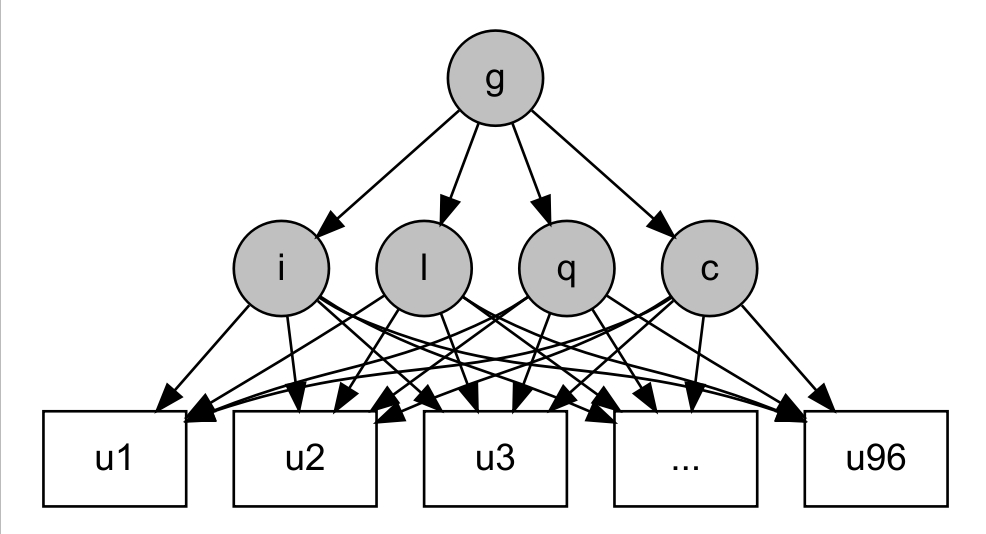
\includegraphics[width=10cm]{Figures/LCGAdiagramme.jpeg}
%	\decoRule
%	\caption[Diagramme for LCGA model]{Diagram for LCGA model.\\ \scriptsize{\textbf{Abbreviations:} g, latent class variable; i, intercept; l, linear term coefficient; q, quadratic term coefficient; c, cubic term coefficient; u1, u2, ... u96, repeated categorical outcomes of eating carbohydrates at each hour/time slots across four days of survey.}}
%	\label{fig:LCGAdiagram}
%\end{figure}\vspace{-0.6cm}
%
%In the NDNS RP data context, we considered a latent categorical variable $g_i$ representing the unobserved subpopulation membership (latent class variable) for participant $i, (g_{i} = 1,2,\cdots K)$. Then a LCGA model predicts the probability of the carbohydrate eating response $u_{ti}$ at time $t$ in latent class $K$ can be written as: \vspace{-0.3cm}
%
%\begin{equation}
%\begin{aligned}
%P(u_{ti} = 0/1/2 |g_i = K) &  = \frac{1}{1 + e^{-\text{logit}(u_{itK})}} \\
%\text{logit}(u_{itK}) & = \beta_{0K} + \beta_{1K}t_{i} + \beta_{2K}t^2_i + \beta_{3K}t^3_i + \epsilon_{i} \\ 
%\epsilon_{i} \sim N(0, \sigma^2) & \;i = 1,2,...6155
%\end{aligned}
%\end{equation}\vspace{-0.6cm}
%
%Where, 
%
%\begin{itemize}
%	\item $u_{ti}=\left\{ \begin{array}{ll}  0 & \text{if particiant } i \text{ was not eating any food at time } t\\ 
%	 1 & \text{if particiant } i \text{ was eating food and contribution of energy} \\ 
%	   &  \text{from carbohydrate was lower than 50\% at time } t \\ 
%	 2 & \text{if participant } i \text{ was eating food and contribution of energy} \\ 
%	 &  \text{from carbohydrate was higher or equal to 50\% at time } t \end{array} \right.$
%	\item $\beta_{0K}, \beta_{1K}, \beta_{2K}, \beta_{3K}$  correspond to $i, l, q, c$ in \textbf{Figure \ref{fig:LCGAdiagram}}, i.e. the coefficients for intercept, linear, quadratic, and cubic term of time.
%\end{itemize}
%
%An LCGA model can be modelled using either a linear, quadratic, or cubic trend over time. However, in our case, it may not be appropriate to assume the probabilities of responses to eating carbohydrates on the logit scale to change on a linear, or quadratic trend over four days, we chose to fit a more flex time function-a cubic form of time. The assumption in a LCGA model is that the data trajectory (the curve of eating carbohydrate pattern) for the participant consisting of the repeated measurements over time $t$, are independent given the group, $g_i$.



\subsection{Characteristics of day level latent classes and individual level latent classes}\vspace{-0.3cm}


Day level latent classes identified by the first step of MLCA were tabulated according to day of week and also whether the diary was recorded during weekends or not. A contingency table giving the frequency of responses across the 7 time slots of the survey days was produced. Descriptive statistics for the dietary day level recordings according to the latent class memberships were presented. Pearson $\chi^2$ test was used to compare the distribution of categorical variables. One-way Analysis of Variance (ANOVA) was used to compare the means across the multiple groups for continuous variables.

Person level point estimates and 95\% confidence intervals (CIs) were determined by applying individual, nurse visiting, and blood sample weights accordingly which account for the probability of participant selection and the clustered survey design. Descriptive statistics for sample characteristics are presented as weighted means (95\% CI) or weighted percentages (95\%CI). After examining the distribution of the data, the following variables were log-transformed to improve normality: fasting blood glucose, A1C, TC, LDL, HDL, TG, and average physical activity duration per day. Weighted geometric means (95\% CI) were used for all log-transformed variables. 

To see whether there is any temporal pattern for food intake eating could also be defined at individual level, weighted estimates of nutrients consumption across the 7 time slots of the day were calculated for each individual level latent class. Contributions (\%) of the average energy intake within time slots were evaluated by determining the percentages of energy coming from carbohydrate, fat, protein, and alcohol intake. 

For continuous variables, the \textit{F} test was used to determine differences between latent classes with Bonferroni correction to account for multiple testing across $>$ 2 classes when applicable. For categorical variables, differences between latent classes were assessed using the adjusted Pearson $\chi^2$ test for survey data.\vspace{-0.5cm}


\subsection{Association between individual level latent classes and the prevalence of hypertension, and measurements of obesity}\vspace{-0.3cm}


Associations between individual level carbohydrate eating classes and hypertension (yes/no), body mass index (BMI, kg/m\textsuperscript{2}), and waist circumference (WC, cm) were explored in men and women separately. Point estimates of weighted means and proportions and 95\%CI of the characteristics were determined by applying either nurse visiting weights (for outcomes of hypertension, BMI, and WC) or blood sample weights (for diagnosis of DM) accordingly. Similarly, \textit{F} tests (for continuous variables) and adjusted Pearson $\chi^2$ tests (for categorical variables) were used to determine sex-specific differences by hypertension status, and BMI categories. 

%multinomial logistic regression model (for BMI categories),


Survey-designed logistic regression models (for hypertension), and linear regression models (for WC, BMI), were used to test for associations between latent classes of carbohydrate eating patterns and hypertension, BMI, and WC, in the NDNS RP sample, separately. Since diabetic participants might or might not modify their carbohydrate eating habits, we also fitted all the above mentioned regression models restricted to those without diabetes.

For the multiple regression models, model fitting strategies are as follows: 

\begin{enumerate}
	\item The crude association between the carbohydrate eating groups and the outcomes was first examined. 
	\item Potential confounders of the association between carbohydrate eating groups (exposure) and the outcomes were selected depending on the descriptive statisitical analyses conducted above, i.e. those are associated with both the exposure and the outcome and also not on the causal pathway were selected as potential confounders. Those are strongly related with the outcomes but may not associated with carbohydrate eating groups may reduce the standard errors and so improve the precisions are also considered in the linear regression models. 
	\item Confounding and/or interaction effect from each of the potential factors were checked one by one. Interaction effect were tested using the adjusted Wald test testing whether the regression coefficients of the interaction terms are simultaneously equal to zero.  
	\item A preliminary model that includes all of the variables suggested to be confounders in the previous step was established. 
	\item The remaining variables were added to the preliminary model one by one to see if any of them may be a confounder in condition of the presence of the other covariates. 
	\item For logistic regression models (hypertension) under the survey data, goodness-of-fit was assessed using the adapted \code{svylogitgof} command in Stata \parencite{archer2006goodness}. Other diagnostics for regular logistic regression models, such as estimating the pseudo-R\textsuperscript{2},  AIC or BIC, checking the standardized Pearson residuals, or covariate pattern residuals are currently not available for weighted survey data. 
	\item For linear regression models (WC, BMI), assumption of independent observations is violated as soon as we weighted the sample. General checking such as QQ plots of the residuals (normality), plotting the residuals against fitted values (constant variance) are not available as well. Outliers, leverage, and Cook's distance cannot be check either, however, participants with extreme weightings (if exist) were checked by removing them and refit the models as a sensitivity analysis.
	\item Since under survey design data, the sampling-weighted least squares are not maximum likelihood, it would not be possible to compare models using likelihood ratio test. Instead, adjusted Wald tests with $p < 0.05$ were used as criteria for variable inclusion in the final model. Another Stata command \code{linktest} was also used to  decide whether quadratic and cubic terms of continuous variables were necessary in improving the fitting of model \parencite{pregibon1980goodness}. 
\end{enumerate}

Data manipulation and preparation \textbf{(Appendix \ref{AppendixA})} were done in R version 3.5.1 \parencite{R3.5.1}. All statistical analyses, except for MLCA models, were performed with \code{svyset} command as implemented in Stata software version 15.1 \parencite{stata15}. The process of model fitting, covariates selection, interaction effect testings for the association between carbohydrate eating patterns and hypertension is shown as an example in \textbf{Appendix \ref{AppendixD}}. All \textit{p} values were two-sided.

% Chapter Template

\chapter{Results} % Main chapter title

\label{Chapter 3} % Change X to a consecutive number; for referencing this chapter elsewhere, use \ref{ChapterX}


\vspace{-0.7cm}

%----------------------------------------------------------------------------------------
%	SECTION 1
%----------------------------------------------------------------------------------------

\subsection{Model selection, and interpretation}\vspace{-0.4cm}

A series of traditional LCA of the responses to carbohydrate intake within 7 time slots of day was first examined. These initial analyses ignored the clustering of observation days within participants of the survey. \textbf{Table \ref{tab:mixmodels}} shows the latent class solutions for one to five classes (see rows under the Fixed effects model section). The BIC declines with the number of day level classes increases. However, the improvement of BIC dropped to less than 1000 from 3 classes to 4 classes solutions (658.9) and from 4 classes to 5 classses solutions (361.7). Entropy index indicates that the 4 classes model could explain about 51\% percent of the data, while \textit{p} values of Lo-Mendell-Rubun LRT suggest that the more classes we fit, the better model we will have until up to 6 classes (\textit{p} = 0.06 and is not shown in the table). From the parsimony point of view, we extended the model with random effects building on 2 classes, 3 classes and 4 classes solutions. 

The results of the random effect included models are presented in \textbf{Table \ref{tab:mixmodels}} under the Random effects model section. It is obvious that the BIC improves with the addition of the random effects which account for the nested structure of the data. Entropy indicates that 4 classes in individual level and 2 classes in the day level may be the best solution mathematically. However, after these solutions were checked in more details, the potentially most substantively interpretable model was found to be the 3$\times$3 random effect model, which is the model with 3 latent classes in the day level, and 3 latent classes in the individual level. We must emphasize that different researchers may have made decision slightly different from ours, we provided the descriptions and figures for other solutions in the \textbf{Appendix \ref{AppendixC}} for reference. 

In the 3$\times$3 random effect model solution we have chosen, there were 39.5\%, 20.4\%, and 40.1\% observations classified into 3 latent groups in the day level. The overall counts and percentages for each responses within every time slot and the distributions of the solution are presented in \textbf{Table \ref{tab:daylevel}}. The trajectories illustrating the change of the probabilities of each response to carbohydrate eating during the hours of the day are shown separately by three types of days in \textbf{Figure \ref{fig:level1}}.



\rowcolors{2}{gray!6}{white}

\begin{table}[H]
	
	\caption{\label{tab:mixmodels}Fit criteria for each model specification.}\vspace{-0.3cm}
	\centering
	\fontsize{9}{11}\selectfont
	\begin{tabular}[t]{lccccc}
		\hiderowcolors
		\toprule
		\multicolumn{1}{c}{ } & \multicolumn{5}{c}{\textbf{Number of day level classes}} \\
		\cmidrule(l{2pt}r{2pt}){2-6}
		\textbf{Model} & \textbf{1 class} & \textbf{2 classes} & \textbf{3 classes} & \textbf{4 classes} & \textbf{5 classes}\\
		\midrule
		\showrowcolors
		\addlinespace[0.3em]
		\multicolumn{6}{l}{\textbf{Fixed effects model}}\\
		\hspace{1em}No. of free parameters & 14 & 29 & 44 & 59 & 74\\
		\hspace{1em}\hspace{1em}Log-likelihood & -173793.306 & -172669.771 & -172039.204 & -171633.941 & -171377.292\\
		\hspace{1em}\hspace{1em}BIC & 347728.092 & 345632.608 & 344523.060 & 343864.121 & 343502.409\\
		\hspace{1em}\hspace{1em}Lo-Mendell-Rubun LRT & -- & $<$ 0.0001 & $<$ 0.0001 & $<$ 0.0001 & $<$ 0.0001\\
		\hspace{1em}\hspace{1em}Entropy & 1 & 0.310 & 0.392 & 0.510 & 0.481\\
		\addlinespace[0.3em]
		\multicolumn{6}{l}{\textbf{Random effects model}}\\
		\hspace{1em}2 individual level classes &  &  &  &  & \\
		\hspace{1em}\hspace{1em}No. of free parameters &  & 59 & 89 & 119 & \\
		\hspace{1em}\hspace{1em}Log-likelihood &  & -169331.132 & -168700.96 & -168366.193 & \\
		\hspace{1em}\hspace{1em}BIC &  & 339258.502 & 338301.338 & 337934.968 & \\
		\hspace{1em}\hspace{1em}Entropy &  & 0.581 & 0.569 & 0.555 & \\
		\hspace{1em}3 individual level classes &  &  &  &  & \\
		\hspace{1em}\hspace{1em}No. of free parameters &  & 89 & 134 & 179 & \\
		\hspace{1em}\hspace{1em}Log-likelihood &  & -166936.279 & -166348.815 & -166062.761 & \\
		\hspace{1em}\hspace{1em}BIC &  & 334771.968 & 334051.799 & 333934.448 & \\
		\hspace{1em}\hspace{1em}Entropy &  & 0.677 & 0.630 & 0.644 & \\
		\hspace{1em}4 individual level classes &  &  &  &  & \\
		\hspace{1em}\hspace{1em}No. of free parameters &  & 119 & 179 &  & \\
		\hspace{1em}\hspace{1em}Log-likelihood &  & -165441.731 & -164845.696 &  & \\
		\hspace{1em}\hspace{1em}BIC &  & 332086.045 & 331500.318 &  & \\
		\hspace{1em}\hspace{1em}Entropy &  & 0.729 & 0.659 &  & \\
		\bottomrule
		\multicolumn{6}{l}{{\scriptsize \textit{Note: }}}\\
		\multicolumn{6}{l}{{\scriptsize \textbf{Abbreviations}: No, number; BIC, Bayesian information criterion; Entropy, a pseudo-r-squared index;}}\\ 
		\multicolumn{6}{l}{{\scriptsize Lo-Mendel-Rubin LRT, likelihood ratio test comparing $q$ classes models with $q-1$ classes models.}}\\
	\end{tabular}
\end{table}

\rowcolors{2}{white}{white}
\vspace{-0.5cm}


Class 1 days \textbf{(Figure \ref{fig:level1}-A)} were given the name of "high percentage carbohydrate day" since in these days of survey, the probabilities of carbohydrate contributed higher or equal to 50\% of the energy consumed were always higher than that in the other two types of days. Specifically, high percentage carbohydrate days were characterised with probabilities of over 0.6 in time slots between 6 am to 9 am, 9 am to 12 noon, and also 2 pm to 5 pm, during which the time slots may be interpreted as breakfast, morning snack, and afternoon snack time periods for many participants. Moreover, even during late night time period, such as 8 pm to 10 pm, and 10 pm to 6 am time slots, the probabilities of having higher carbohydrate contained food were still as high as 0.412, and 0.246, respectively.



\rowcolors{2}{gray!6}{white}

\begin{table}[H]
	
	\caption{\label{tab:daylevel}Day level latent class solution for three classes LCA model. (No individual level model)}\vspace{-0.3cm}
	\centering
	\fontsize{9}{11}\selectfont
	\begin{tabular}[t]{llccccc}
		\hiderowcolors
		\toprule
		\textbf{Time slots of} & \textbf{Responses to} & \multicolumn{1}{c}{ } & \multicolumn{1}{c}{ } & \textbf{\Centerstack{Class 1 days\\(39.5\%)}} & \textbf{\Centerstack{Class 2 days\\(20.4\%)}} & \textbf{\Centerstack{Class 3 days\\(40.1\%)}} \\
		\cmidrule(l{2pt}r{2pt}){5-5} \cmidrule(l{2pt}r{2pt}){6-6} \cmidrule(l{2pt}r{2pt}){7-7}
		 \textbf{the day} &  \textbf{carbohydrate intake} & $n$ & (\%) & \textbf{\Centerstack{High perc-\\entage carb}} & \textbf{\Centerstack{Low perc-\\entage carb}} & \textbf{\Centerstack{Regular\\meals}}\\
		\midrule
		\showrowcolors
		6 am – 9 am &  &  &  &  &  & \\
		& Not eating any food & 7655 & 31.2 & 0.129 & 0.450 & 0.320\\
		& Carbohydrate $<$ 50\%\textsuperscript{*} & 4500 & 18.4 & 0.130 & 0.267 & 0.128\\
		& Carbohydrate $\geqslant$ 50\%\textsuperscript{\dag} & 12328 & 50.4 & 0.741 & 0.283 & 0.552\\
		9 am – 12 noon &  &  &  &  &  & \\
		& Not eating any food & 5447 & 22.2 & 0.237 & 0.079 & 0.401\\
		& Carbohydrate $<$ 50\% & 7227 & 29.5 & 0.158 & 0.492 & 0.173\\
		& Carbohydrate $\geqslant$ 50\% & 11809 & 48.2 & 0.605 & 0.429 & 0.426\\
		12 noon – 2 pm &  &  &  &  &  & \\
		& Not eating any food & 4783 & 19.5 & 0.156 & 0.356 & 0.019\\
		& Carbohydrate $<$ 50\% & 11112 & 45.4 & 0.405 & 0.413 & 0.560\\
		& Carbohydrate $\geqslant$ 50\% & 8588 & 35.1 & 0.439 & 0.231 & 0.421\\
		2 pm – 5 pm &  &  &  &  &  & \\
		& Not eating any food & 6926 & 28.3 & 0.130 & 0.123 & 0.659\\
		& Carbohydrate $<$ 50\% & 8277 & 33.8 & 0.249 & 0.602 & 0.076\\
		& Carbohydrate $\geqslant$ 50\% & 9280 & 37.9 & 0.621 & 0.276 & 0.266\\
		5 pm – 8 pm &  &  &  &  &  & \\
		& Not eating any food & 3043 & 12.4 & 0.114 & 0.199 & 0.034\\
		& Carbohydrate $<$ 50\% & 14240 & 58.2 & 0.516 & 0.590 & 0.639\\
		& Carbohydrate $\geqslant$ 50\% & 7200 & 29.4 & 0.370 & 0.211 & 0.328\\
		8 pm – 10 pm &  &  &  &  &  & \\
		& Not eating any food & 8722 & 35.6 & 0.322 & 0.291 & 0.480\\
		& Carbohydrate $<$ 50\% & 8898 & 36.3 & 0.266 & 0.551 & 0.212\\
		& Carbohydrate $\geqslant$ 50\% & 6863 & 28.0 & 0.412 & 0.158 & 0.308\\
		10 pm – 6 am &  &  &  &  &  & \\
		& Not eating any food & 16295 & 66.6 & 0.680 & 0.590 & 0.751\\
		& Carbohydrate $<$ 50\% & 4144 & 16.9 & 0.074 & 0.294 & 0.101\\
		& Carbohydrate $\geqslant$ 50\% & 4044 & 16.5 & 0.246 & 0.115 & 0.148\\
		\bottomrule
		\multicolumn{7}{l}{{\scriptsize \textit{Note: }}}\\
		\multicolumn{7}{l}{\scriptsize \textbf{Abbreviation:} LCA, latent class analysis, carb is short for carbohydrates.}\\
		\multicolumn{7}{l}{{\scriptsize \textsuperscript{*} Carbohydrate $<$ 50\% indicates that within the time slot, carbohydrate contributed $<$ 50\% total energy intake.}}\\
		\multicolumn{7}{l}{{\scriptsize \textsuperscript{\dag} Carbohydrate $\geqslant$ 50\% indicates that within the time slot, carbohydrate contributed $\geqslant$ 50\% total energy intake.}}\\
		\multicolumn{7}{l}{}\\ 
	\end{tabular}
\end{table}

\rowcolors{2}{white}{white}
\vspace{-0.6cm}

Class 2 days \textbf{(Figure \ref{fig:level1}-B)} were named as "low percentage carbohydrate day" because first of all, in these days the probability of participants skipping breakfast was 0.45. And after 9 am, within these days, the probability of having low carbohydrate contained food (carbohydrate contributed $<$ 50\% of total energy intake), was always higher than having high carbohydrate contained food (carbohydrate contributed $\geqslant$ 50\% of total energy intake). In class 2 days, participants also turned to have morning snacks (with only 0.079 possibility of \textbf{not} eating any food and similar probabilities of having either high or low carbohydrate contained food). This phenomenon may also be interpreted as having a long and late breakfast (brunch) in these mornings. The probability of \textbf{not} eating any food was the lowest for low carbohydrate days during the midnight time slot (10 pm to 6 am), with probability of 0.590 compared with 0.680 and 0.751 in class 1 and class 3 days, respectively. 





\begin{figure}[H]
	%\vspace*{13cm}
	\centering
	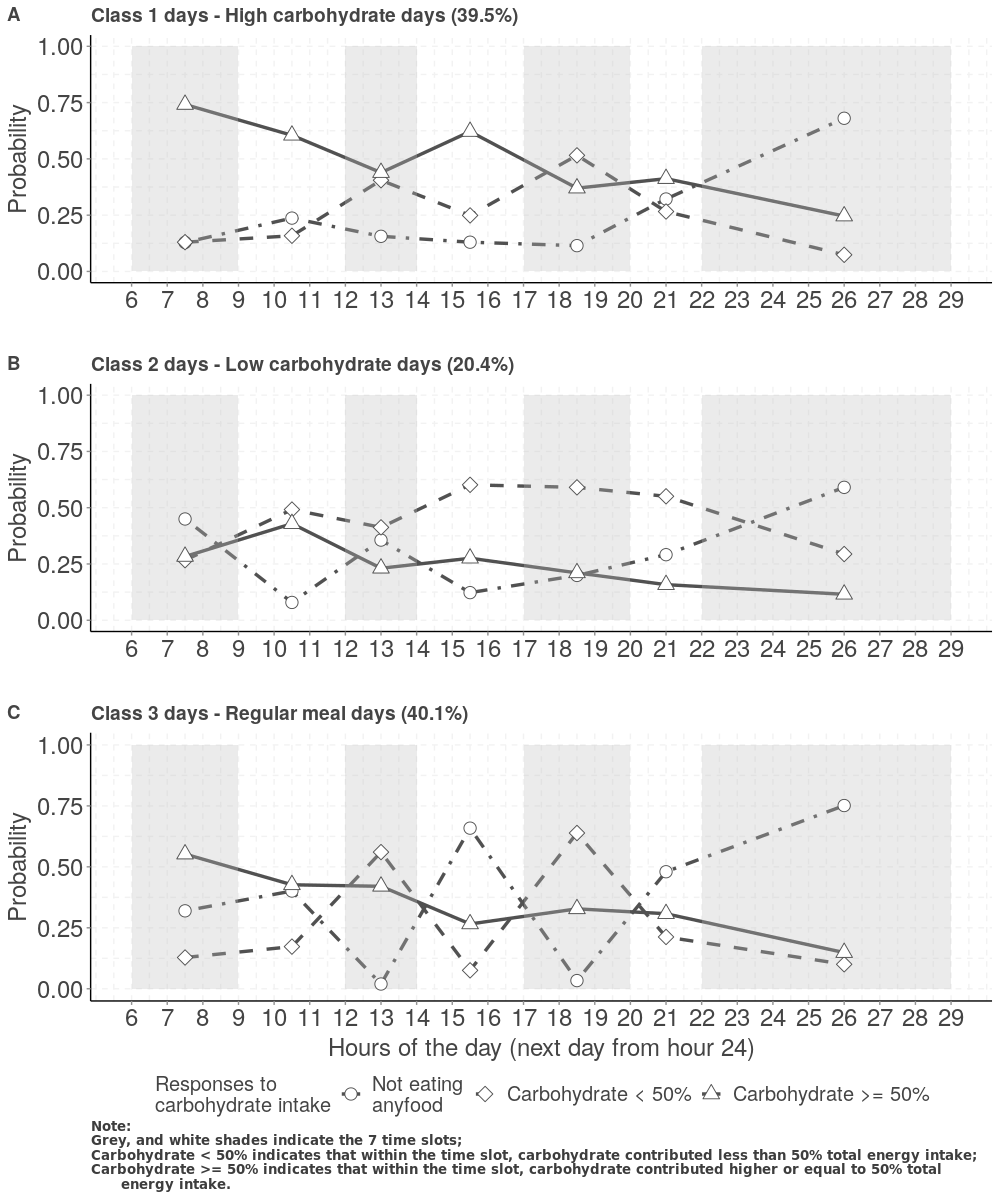
\includegraphics[width=13cm]{Figures/level1.png}
	\decoRule
	\caption[Day Level Latent Class Solution.]{Day Level Latent Classes Solution.}
	\label{fig:level1}
\end{figure}
\vspace{-0.6cm}

Class 3 days \textbf{(Figure \ref{fig:level1}-C)} were called "regular meals day" due to the following reasons: 1) participants' dietary recordings showed that in these days there was almost 0 possibility of not eating any food at lunch (0.019 between 12 noon and 2 pm) and dinner (0.034 between 5 pm and 8 pm); 2) the probabilities of not eating during morning snack time (9 am to 12 noon) and afternoon snack time (2 pm to 5 pm) were also the highest among the three types of days (0.401 and 0.659). 3) during these days, participants may have some high carbohydrate contained food between 8 pm and 10 pm (probability = 0.308), but the probability of not eating any food during 10 pm to 6 am next morning was 0.751, the highest among the three types of days. \vspace{-0.5cm}


\subsection{Features of the three types of carbohydrate eating temporal patterns}

\rowcolors{2}{gray!6}{white}

\begin{table}
	
	\caption{\label{tab:day-level-features}Means (standard deviations), and counts (\%) of the characteristics of different types of carbohydrate eating days.}\vspace{-0.3cm}
	\centering
	\fontsize{9}{11}\selectfont
	\begin{tabular}[t]{lcccc}
		\hiderowcolors
		\toprule
		& \textbf{\Centerstack{High perc-\\entage carb}} & \textbf{\Centerstack{Low perc-\\entage carb}} & \textbf{\Centerstack{Regular\\meals}} & \textbf{\textit{P} value}\textsuperscript{*}\\
		\midrule
		\showrowcolors
		Counts (\%) & 9667 (39.5) & 5002 (20.4) & 9814 (40.1) & \\
		Country (\%) &  &  &  & < 0.001\\
		\hspace{1em}England & 5627 (58.2) & 2972 (59.4) & 5291 (53.9) & \\
		\hspace{1em}Northern Ireland & 1194 (12.4) & 527 (10.5) & 1400 (14.3) & \\
		\hspace{1em}Scotland & 1527 (15.8) & 813 (16.3) & 1774 (18.1) & \\
		\hspace{1em}Wales & 1318 (13.6) & 690 (13.8) & 1349 (13.7) & \\
		Day of Week (\%) &  &  &  & < 0.001\\
		\hspace{1em}Monday & 1303 (13.5) & 715 (14.3) & 1370 (14.0) & \\
		\hspace{1em}Tuesday & 1266 (13.1) & 674 (13.5) & 1290 (13.1) & \\
		\hspace{1em}Wednesday & 1225 (12.7) & 740 (14.8) & 1233 (12.6) & \\
		\hspace{1em}Thursday & 1272 (13.2) & 752 (15.0) & 1425 (14.5) & \\
		\hspace{1em}Friday & 1458 (15.1) & 797 (15.9) & 1479 (15.1) & \\
		\hspace{1em}Saturday & 1537 (15.9) & 703 (14.1) & 1495 (15.2) & \\
		\hspace{1em}Sunday & 1605 (16.6) & 621 (12.4) & 1522 (15.5) & \\
		\hspace{1em}Weekend, Yes (\%) & 3142 (32.5) & 1324 (26.5) & 3017 (30.7) & < 0.001\\
		Total energy (kJ) & 7539.98 (2875.87) & 7160.22 (2922.15) & 7439.68 (2978.91) & < 0.001\\
		Carbohydrate (g) & 222.79 (89.84) & 209.70 (86.17) & 206.59 (84.42) & < 0.001\\
		Protein (g) & 71.36 (29.79) & 69.55 (30.20) & 73.29 (32.94) & < 0.001\\
		Fat (g) & 65.44 (33.27) & 63.94 (33.76) & 67.24 (34.73) & < 0.001\\
		Alcohol (g) & 11.76 (27.31) & 8.85 (24.25) & 13.80 (33.00) & < 0.001\\
		Total sugars (g) & 98.63 (56.03) & 88.03 (50.50) & 86.39 (50.96) & < 0.001\\
		Starch (g) & 124.07 (55.84) & 121.59 (56.13) & 120.11 (54.62) & < 0.001\\
		Non-milk extrinsic sugar\textsuperscript{\dag} & 59.45 (49.31) & 50.07 (43.41) & 50.41 (44.84) & < 0.001\\
		Fruit (g) & 107.40 (137.97) & 103.15 (129.08) & 92.76 (126.02) & < 0.001\\
		Yellow Red Green Vegetables (g) & 26.52 (46.44) & 26.84 (47.99) & 26.16 (45.99) & 0.681\\
		\bottomrule
		\multicolumn{5}{l}{{\scriptsize \textit{Note:} carb is short for carbohydrate.}}\\
		\multicolumn{5}{l}{{\scriptsize \textsuperscript{*} \textit{P} values were obtained from Pearson $\chi^2$ test for categorical variables, and one-way ANOVA comparing the means}}\\
		\multicolumn{5}{l}{{\scriptsize  in multiple groups for continuous variables;}}\\
		\multicolumn{5}{l}{{\scriptsize \textsuperscript{\dag} Non-milk extrinsic sugar is defined as: additionally added free sugar, such as table sugar, honey, glucose, fructose}}\\ 
		\multicolumn{5}{l}{{\scriptsize and glucose syrups, sugars added to food and sugars in fruit juices.}}\\
	\end{tabular}
\end{table}

\rowcolors{2}{white}{white}
\vspace{-0.5cm}

The details of the characteristics of the three types of carbohydrate eating time pattern were listed in\textbf{ Table \ref{tab:day-level-features}}. Specifically, regular meals day turned to be recorded slightly more often in Northern Ireland, and Scotland. In terms of day of week distribution in the three types of days, there is strong evidence (\textit{p} < 0.001) that high carbohydrate days appeared more frequently in weekends (32.5\%) compared with low carbohydrate day (26.5\%) and regular meals day (30.7\%).

As expected, consumption of total energy (7539.98 kJ), total carbohydrate (222.79 g), total sugar (98.63 g), starch (124.07 g), and non-milk extrinsic sugar (59.45 g) were the highest among high percentage carbohydrate days (all \textit{p} < 0.001). On the other hand, the consumption of protein (73.29 g), total fat (67.24 g), and alcohol (13.80 g) were the highest in the regular meals days. Moreover, in high percentage carbohydrate days, participants turned to consume the highest amount of fruit (107.40 g). There was no evidence of any difference for the consumption of yellow, red, or green vegetables across the three types of days (\textit{p} = 0.681).\vspace{-0.6cm}

%---------------------------------
%	SUBSECTION 2
%-----------------------------------

\subsection{Individual level LCA solution}\vspace{-0.3cm}

In the random effect models we utilized the non-parametric approach, in which we added a level 2 (individual level) latent classes based on the random means from the level 1 (day level) latent class solution. The results of the individual level LCA solution for 2 and 3 classes are presented in \textbf{Figure \ref{fig:CB2level2}}, and \textbf{\ref{fig:level2}}. 


\begin{figure}[H]
	%\vspace*{13cm}
	\centering
	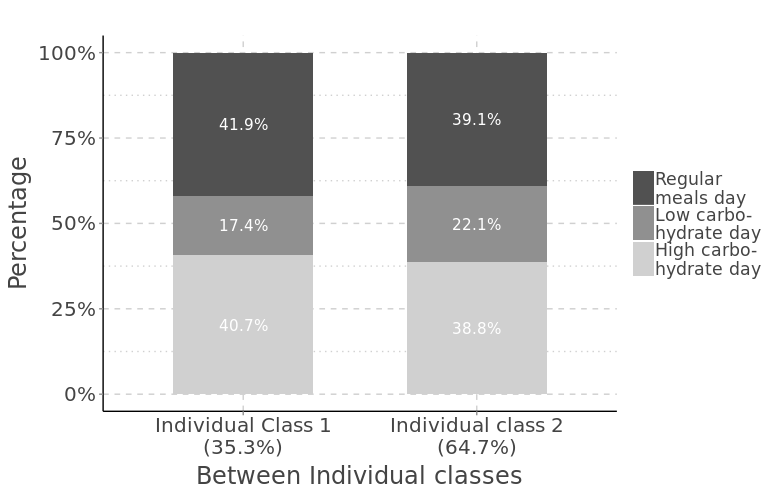
\includegraphics[width=11cm]{Figures/CB2level2.png}
	\decoRule
	\caption[Multilevel Latent Class Solution ($3\times2$).]{Multilevel Latent Class Solution, 3 classes in day level, 2 classes in individual level.}
	\label{fig:CB2level2}
\end{figure}

With two individual level latent classes \textbf{(Figure \ref{fig:CB2level2})}, one individual class is comprised of individuals with a relatively slightly higher proportion of having "low carbohydrate day" (22.1\%) compared to the other (17.4\%). This class represents nearly 65\% of the individuals. However, we believe these individual classes are not very distinguishable to each other.

With three individual level latent classes \textbf{(Figure \ref{fig:level2})}, a low-carbohydrate eaters class, a moderate-carbohydrate eaters class, and a high-carbohydrate eaters class emerges. 43.1\% participants were identified as high-carbohydrate eaters, in these individuals, about 50\% of the days (2 out of 4 days) of their dietary diary could be classified as having high carbohydrate days. Nearly 1 out of 4 days of their dietary diary were either "regular meals day" or "low carbohydrate day". 28.1\% participants fell into the low carbohydrate eaters class in the left hand side of \textbf{Figure \ref{fig:level2}}, their recordings of food intake showed that in more than 60\% of their days, they were having "regular meals" which was characterised as with highest amount of fat and alcohol consumptions as already described in \textbf{Table \ref{tab:day-level-features}}. Moderate carbohydrate eaters have comparable proportions (42.0\% vs. 40.0\%) of having high carbohydrate days and regular meals day, 18.0\% of their dietary diary were found to be low carbohydrate days.

\begin{figure}
	%\vspace*{13cm}
	\centering
	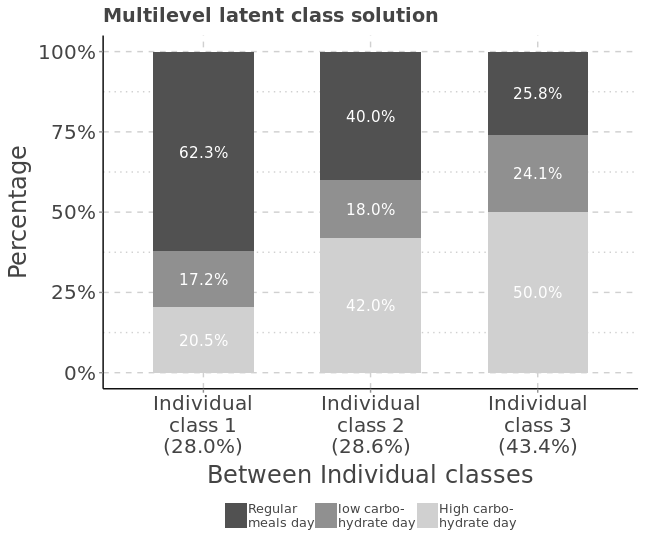
\includegraphics[width=11cm]{Figures/level2.png}
	\decoRule
	\caption[Multilevel Latent Class Solution ($3\times3$).]{Multilevel Latent Class Solution, 3 classes in day level, 3 classes in individual level.}
	\label{fig:level2}
\end{figure}

After recognising that there were three potential latent groups of carbohydrate eaters in the UK adults, whose food consumption pattern were also probably switching from one to another during the survey, their average carbohydrate contribution to total energy intake (as well as the subtypes of carbohydrate actually consumed) within the 7 pre-defined time slots of the day were still of interest. Survey-design-weighted mean energy intake within each time slot of the day and their composition of contribution are illustrated in \textbf{Figure \ref{fig:energysourcesCB}}, weighted mean nutrients intakes are listed in \textbf{Table \ref{tab:tab-nutri-indi}}.

\begin{figure}[H]
	%\vspace*{13cm}
	\centering
	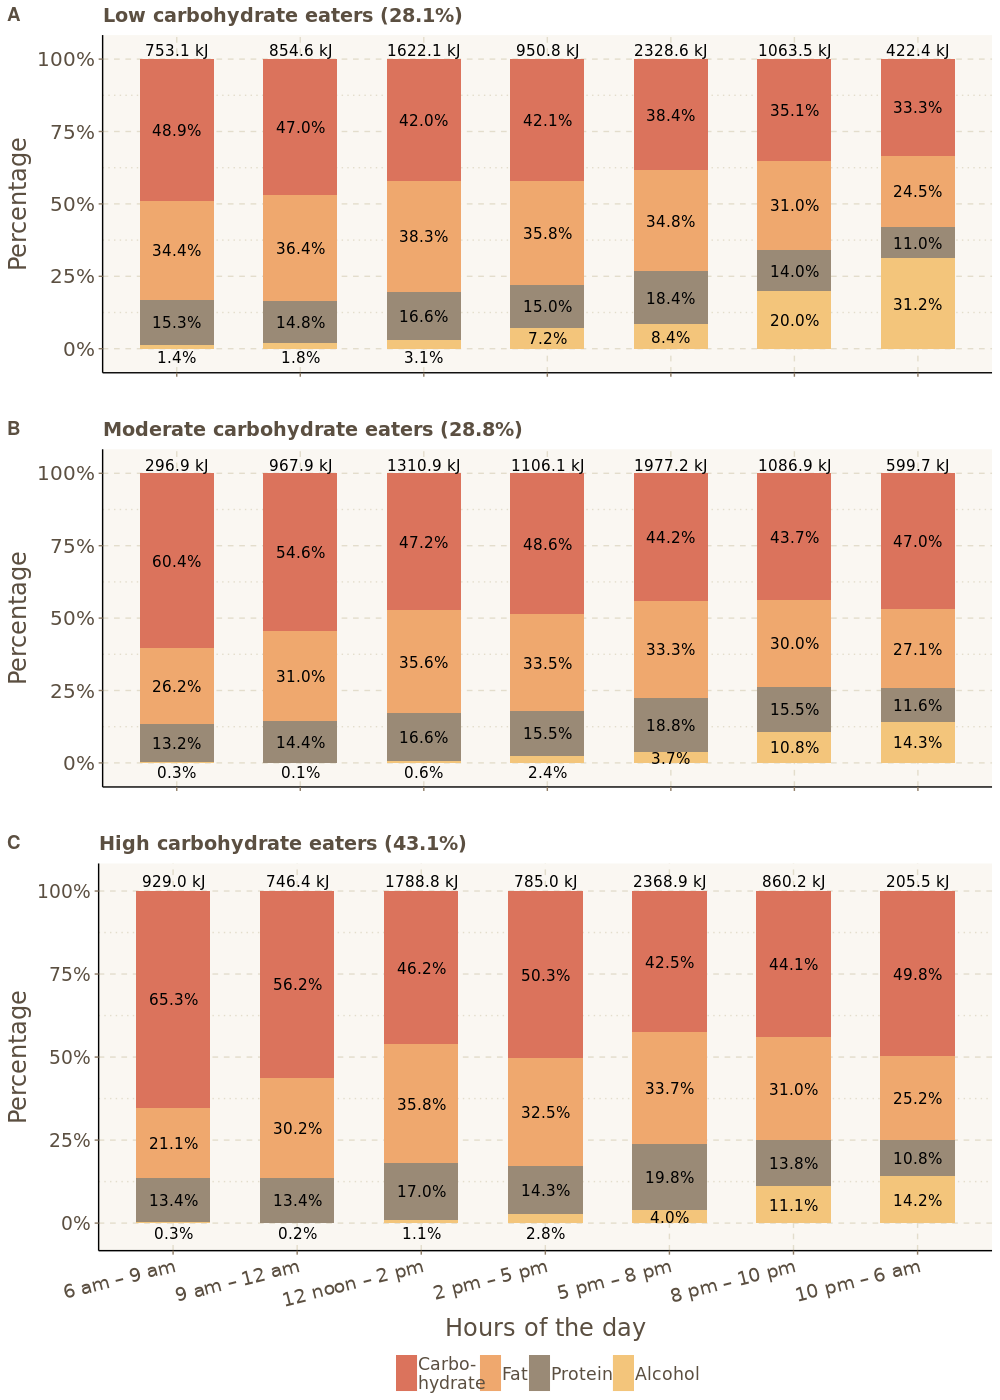
\includegraphics[width=13cm]{Figures/CBenergysources.png}
	\decoRule
	\caption[Sources of Energy Contribution at Each Time Slot by Individual Carbohydrate Eating Groups.]{Sources of Energy Contribution at Each Time Slot by Individual Carbohydrate Eating Groups.}
	\label{fig:energysourcesCB}
\end{figure}
\vspace{-0.6cm}

Among the three types of carbohydrate eaters, the mean of total energy intake over the 4 days of dietary survey was the highest (7985.8 kJ, 95\%CI: 7283.3, 8146.3) in the low carbohydrate eaters group, and the lowest (7341.8 kJ, 95\%CI: 7172.5, 7511.2) in the moderate eaters group \textbf{(Table \ref{tab:tab-nutri-indi})}. Sources of energy for each type of carbohydrate eaters by the 7 time slots were also different. Low carbohydrate eaters \textbf{(Figure \ref{fig:energysourcesCB}-A)} never had carbohydrate contributed more than 50\% of their total energy throughout the day. Energy from fat were the highest for low carbohydrate eaters most of the time during the day (except for time between 10 pm to 6 am next morning). Most impressively, energy from alcohol were always the highest in low carbohydrate eaters, percentages for energy from alcohol for the 7 times slots were 1.4\% (6-9 am), 1.8\% (9-12 noon), 3.1\% (12-2 pm), 7.2\% (2-5 pm), 8.4\% (5-8 pm), 20.0\% (8-10 pm), and 31.2\% (10 - 6 am), respectively. Contribution from different energy sources are quite similar for moderate and high carbohydrate eaters, but their absolute amount of energy consumption at each time slot were largely different. Moderate carbohydrate eaters \textbf{(Figure \ref{fig:energysourcesCB}-B)} were characterised as consuming the lowest energy (296.9 kJ) before 9 am, but having higher energy consumption (967.9 kJ) between 9 am and 12 noon time compared with low and high carbohydrate eaters. Moderate carbohydrate eaters may turn to have later breakfast, later lunch, and probably later dinner as well. They had the highest total energy consumption (599.7 kJ) at night (10 pm - 6 am) across three types of eaters. High carbohydrate eaters \textbf{(Figure \ref{fig:energysourcesCB}-C)} consumed the highest total energy (929.0 kJ) during 6 am to 9 am in the morning and the lowest total energy between 10 pm to 6 am (205.5 kJ). Specifically, carbohydrate contribution to total energy intake were 65.3\% (6-9 am), 56.2\% (9-12 noon), 46.2\% (12-2 pm), 50.3\% (2-5 pm), 42.5\% (5-8 pm), 44.1\% (8-10 pm), and 49.9\% (10-6am). We also noticed that high carbohydrate eaters consumed their energy mainly from three time slots: 6-9 am, 12-2 pm, and 5-8 pm. 

As expected, in total, the mean of carbohydrate intake was 203.8 g, 218.3 g, and 233.4 g for low, moderate, and high carbohydrate eaters, respectively \textbf{(Table \ref{tab:tab-nutri-indi})}. Energy contribution from carbohydrate was close to 50\% in the high carbohydrate eaters, but was only 40.6\% in the low carbohydrate eaters. In terms of the subtypes (components) of the carbohydrate consumed at each time slot, high carbohydrate eaters consumed as much as more than 2 times (compared to low carbohydrate eaters) and nearly 4 times (against moderate carbohydrate eaterss) the amount of sugar (37.9g 95\% CI: 36.8, 39.2) and non-milk extrinsic sugar (i.e. free sugar) (11.1g 95\%CI: 10.7, 11.6) between 6-9 am. Moderate carbohydrate eaters had their carbohydrate intake more spread out. They consumed more sugar and starch during 9-12 noon, 2-5 pm, 8-10 pm, and 10-6 am. Low carbohydrate eaters turned to have similar temporal pattern of consuming carbohydrates but the absolute amount of fibre, sugar, free sugar, and starch were usually lower than that in the high carbohydrate eaters except for time slots of 2-5 pm, and 10-6 am. Strong evidence (\textit{p} < 0.001) suggested that the mean of total fibre consumption for low,




\rowcolors{2}{gray!6}{white}

\begin{table}[H]
	
	\caption{\label{tab:tab-nutri-indi}Weighted means and percentages (95\%CI) of the nutrients intake according to individual level carbohydrate eating classes.  \\ (NDNS RP 2008/09-15/16, sample size = 6155)}\vspace{-0.3cm}
	\centering
	\fontsize{9}{11}\selectfont
	\begin{tabular}[t]{lcccc}
		\hiderowcolors
		\toprule
	\textbf{Variables} & \textbf{\Centerstack{Low carbo-\\hydrate eaters\\(n = 1730)}} & \textbf{\Centerstack{Moderate carbo-\\hydrate eaters\\(n = 1772)}} & \textbf{\Centerstack{High carbo-\\hydrate eaters\\(n = 2653)}} & \textbf{\textit{P} value} \textsuperscript{*}\\
		\midrule
		\showrowcolors
		Total energy (kJ) & 7985.8 (7823.3, 8146.3) & 7341.8 (7172.5, 7511.2) & 7677.8 (7555.8, 7799.8) & < 0.001\\
		Carbohydrate (g) & 203.8 (199.8, 207.8) & 218.3 (212.9, 223.7) & 233.4 (229.6, 237.2) & < 0.001\\
		\hspace{1em}\textbf{6 am – 9 am} & 23.0 (21.8,  24.3) & 11.2 (10.0, 12.3) & 37.9 (36.8, 39.2) & \\
		\hspace{2em}Fibre (g) & 1.4 (1.3, 1.5) & 0.6 (0.5, 0.7) & 2.0 (1.9, 2.2) & \\
		\hspace{2em}Sugar (g) & 10.2 (9.6, 10.9) & 5.3 (4.8, 5.8) & 19.7 (19.0, 20.4) & \\
		\hspace{3em}NMES (g)\textsuperscript{\dag} & 4.7 (4.3, 5.1) & 3.2 (2.9, 3.6) & 11.1 (10.7, 11.6) & \\
		\hspace{2em}Starch (g) & 12.8 (12.0, 13.5) & 5.9 (5.1, 6.6) & 18.3 (17.6, 19.1) & \\
		\hspace{1em}\textbf{9 am – 12 noon} & 25.1 (23.9, 26.3) & 33.0 (31.4, 34.6) & 26.2 (25.1, 27.2) & \\
		\hspace{2em}Fibre (g) & 1.5 (1.4, 1.6) & 1.6 (1.5, 1.7) & 1.3 (1.2, 1.3) & \\
		\hspace{2em}Sugar (g) & 11.6 (10.9, 12.3) & 15.7 (14.8, 16.6) & 14.2 (13.6, 14.8) & \\
		\hspace{3em}NMES (g)\textsuperscript{\dag} & 5.7 (5.2, 6.2) & 9.6 (8.9, 10.2) & 8.1 (7.7, 8.5) & \\
		\hspace{2em}Starch (g) & 13.5 (12.8, 14.3) & 17.3 (16.4, 18.3) & 11.9 (11.3, 12.6) & \\
		\hspace{1em}\textbf{12 noon – 2 pm} & 42.6 (40.9, 44.3) & 38.7 (37.0, 40.4) & 51.6 (50.2, 52.9) & \\
		\hspace{2em}Fibre (g) & 3.1 (2.9, 3.2) & 2.3 (2.2, 2.5) & 3.6 (3.5, 3.7) & \\
		\hspace{2em}Sugar (g) & 14.7 (14.0, 15.4) & 14.9 (14.0, 15.7) & 19.4 (18.7, 20.0) & \\
		\hspace{3em}NMES (g)\textsuperscript{\dag} & 7.3 (6.7, 7.8) & 9.1 (8.4, 9.8) & 10.3 (9.8, 10.8) & \\
		\hspace{2em}Starch (g) & 27.9 (26.6, 29.1) & 23,8 (22.6, 24.9) & 32.2 (31.2, 33.1) & \\
		\hspace{1em}\textbf{2 pm – 5 pm} & 25.0 (23.6, 26.4) & 33.6 (31.6, 35.6) & 24.7 (23.6, 25.7) & \\
		\hspace{2em}Fibre (g) & 1.6 (1.5, 1.7) & 1.9 (1.7, 2.0) & 1.3 (1.2, 1.4) & \\
		\hspace{2em}Sugar (g) & 11.9 (11.3, 12.7) & 14.5 (13.5, 15.5) & 13.4 (12.8, 13.9) & \\
		\hspace{3em}NMES (g)\textsuperscript{\dag} & 6.9 (6.4, 7.5) & 9.9 (9.0, 8.6) & 8.6 (8.2, 9.1) & \\
		\hspace{2em}Starch (g) & 13.1 (12.1, 13.9) & 19.1 (17.7, 20.4) & 11.3 (10.6, 11.9) & \\
		\hspace{1em}\textbf{5 pm – 8 pm} & 55.9 (54.1, 57.9) & 54.6 (52.1, 57.0) & 62.9 (61.3, 64.4) & \\
		\hspace{2em}Fibre (g) & 4.4 (4.2, 4.5) & 3.7 (3.5, 3.9) & 4.9 (4.7, 5.0) & \\
		\hspace{2em}Sugar (g) & 18.7 (17.9, 19.5) & 18.6 (17.6, 19.5) & 21.8 (20.9, 22.5) & \\
		\hspace{3em}NMES (g)\textsuperscript{\dag} & 10.2 (9.6, 10.8) & 11.8 (10.9, 12.6) & 12.1 (11.4, 12.7) & \\
		\hspace{2em}Starch (g) & 37.3 (35.8, 38.8) & 35.9 (34.1, 37.9) & 41.1 (39.9, 42.2) & \\
		\hspace{1em}\textbf{8 pm – 10 pm} & 23.3 (21.9, 24.6) & 29.7 (27.6, 31.7) & 23.7 (22.5, 24.9) & \\
		\hspace{2em}Fibre (g) & 1.4 (1.3, 1.6) & 1.6 (1.5, 1.8) & 1.3 (1.5, 1.8) & \\
		\hspace{2em}Sugar (g) & 10.9 (10.3, 11.5) & 13.2 (12.2, 14.2) & 12.4 (11.8, 13.0) & \\
		\hspace{3em}NMES (g)\textsuperscript{\dag} & 7.3 (6.8, 7.8) & 9.4 (8.5, 10.4) & 8.3 (7.8, 8.8) & \\
		\hspace{2em}Starch (g) & 12.3 (11.4, 13.3) & 16.4 (15.0, 17.8) & 11.3 (10.5, 12.1) & \\
		\hspace{1em}\textbf{10 pm – 6 am} & 8.8 (7.7, 9.8) & 17.6 (15.2, 19.9) & 6.4 (5.8, 7.1) & \\
		\hspace{2em}Fibre (g) & 0.34 (0.29, 0.39) & 0.74 (0.63, 0.85) & 0.24 (0.21, 0.27) & \\
		\hspace{2em}Sugar (g) & 5.3 (4.6, 6.1) & 10.0 (8.6, 11.5) & 4.1 (3.7, 4.5) & \\
		\hspace{3em}NMES (g)\textsuperscript{\dag} & 3.9 (3.3, 4.6) & 7.7 (6.4, 8.9) & 2.9 (2.6, 3.3) & \\
		\hspace{2em}Starch (g) & 3.5 (2.9, 3.9) & 7.5 (6.3, 8.8) & 2.3 (1.9, 2.7) & \\
		Carbohydrate (\%) & 40.6 (40.2, 41.0) & 47.3 (46.8, 47.8) & 48.3 (47.9, 48.6) & < 0.001\\
		Fibre (g) & 13.7 (13.4, 14.0) & 12.5 (12.1, 12.9) & 14.7 (14.4, 14.9) & < 0.001 \\
		Protein (g) & 79.9 (77.9, 81.8) & 69.3 (67.6, 71.0) & 73.7 (72.5, 74.8) & < 0.001\\
%		Protein (\%) & 17.2 (16.9, 17.5) & 16.3 (16.0, 16.6) & 16.5 (16.3, 16.6) & < 0.001\\
		Fat (g) & 74.7 (73.1, 76.4) & 63.8 (62.1, 65.5) & 65.7 (64.4, 67.0) & < 0.001\\
%		Fat (\%) & 35.4 (34.9, 35.8) & 32.5 (32.1, 32.9) & 32.0 (31.7, 32.3) & < 0.001\\
		Alcohol (g) & 20.8 (18.3, 23.2) & 10.7 (9.4, 11.9) & 8.9 (8.1, 9.8) & < 0.001\\
		\bottomrule
		\multicolumn{5}{l}{{\scriptsize \textsuperscript{*} \textit{P} values were obtained from $\chi^2$ test for categorical variables, and one-way ANOVA comparing the means}}\\
		\multicolumn{5}{l}{{\scriptsize  in multiple groups for continuous variables;}}\\
		\multicolumn{5}{l}{\textsuperscript{\dag} NMES, Non-milk extrinsic sugar is defined as: additionally added free sugar, such as table sugar, honey, }\\
		\multicolumn{5}{l}{{\scriptsize glucose, fructose and glucose syrups, sugars added to food and sugars in fruit juices.}}\\
	\end{tabular}
\end{table}

\rowcolors{2}{white}{white}

moderate, and high carbohydrate eaters were different: 13.7g (13.4, 14.0), 12.5g (12.1, 12.9), and 14.7g (14.4, 14.9) with all 95\% CI being exclusive to each other. It is also noteworthy that low carbohydrate eaters consumed the highest average amount of protein (79.9 g, 17.2\% of total energy), fat (74.7g, 35.4\% of total energy), and alcohol (20.8 g, 6.8\% of total energy) as we have described for \textbf{Figure \ref{fig:energysourcesCB}}. 
 
The social-demographic characteristics of the UK adults according to their individual level latent class membership are shown in \textbf{Table \ref{tab:Level2tab1}}. Moderate carbohydrate eaters were relatively younger (\textit{p} < 0.001), and slightly less from England (\textit{p} = 0.007). Gender distribution across the three types of carbohydrate eaters was fairly even (\textit{p} = 0.119). The distribution of the carbohydrate eater types turned out to be changing with the year of survey. Low carbohydrate eaters represented 32.5\% of the population in the first year of survey, but later dropped to lower than 30\% (lowest in the third year, 22.6\%) until the most recent year. Proportion of high carbohydrate eaters increased from 41.2\% to the highest (50.6\%) in the second year, but then started to decline to 38.4\% in the 8th year of survey (\textit{p} = 0.015). There was no evidence of difference in employment status across three types of carbohydrate eaters. However, strong evidence suggested that high carbohydrate eaters had the highest proportion (61.3\%) of living with partner (\textit{p} < 0.001); moderate carbohydrate eaters had the lowest average income (27180.8 \textsterling/year), highest proportion of non-white population (20.5\%), and lower education level (23.3\% with degree of higher education) compared with either low or high carbohydrate eaters. 


Weighted means, percentages of anthropometric measurements, average of main nutrients intake, as well as biochemical characteristic profiles according to the latent carbohydrate eater groups are given in \textbf{Table \ref{tab:tab2}}. Low carbohydrate eaters had higher mean BMI (27.8 kg/m\textsuperscript{2}) and larger mean WC (98.9/89.9 cm in men/women) compared with 27.2, 27.3 kg/m\textsuperscript{2}, and 95.9/88.7 (men/women), 98.1/87.2 (men/women) cm in moderate and high carbohydrate eaters. Moderate carbohydrate eaters had the highest prevalence of being a current smoker (27.8\%), shortest time of daily physical activity (geometric mean: 0.87 hours/day), and the lowest prevalence of hypertension (20.2\%).

From the results of blood tests, 6.9\% of low carbohydrate eaters were found to be diabetic (diagnosed by A1C > 6.5\%), while the percentages of diabetes in the moderate and high carbohydrate eaters were 3.5\%, and 4.1\% (\textit{p} < 0.011), respectively. Although there was some evidence (\textit{p} = 0.027) that fasting blood glucose level may be slightly higher in non-diabetic low carbohydrate eaters, the geometric mean for


\rowcolors{2}{gray!6}{white} 

\begin{table}[H]

\caption{\label{tab:Level2tab1}Weighted means, percentages, and
95\% CIs of the social-demographic characteristics by carbohydrate eating latent class memberships in the UK
adults. \\ (NDNS RP 2008/09-15/16, sample size = 6155)} \centering
\fontsize{9}{11}\selectfont

\begin{tabular}[t]{lcccc}
	\hiderowcolors
	\toprule
	\textbf{Variables} & \textbf{\Centerstack{Low carbo-\\hydrate eaters\\(n = 1730)}} & \textbf{\Centerstack{Moderate carbo-\\hydrate eaters\\(n = 1772)}} & \textbf{\Centerstack{High carbo-\\hydrate eaters\\(n = 2653)}} & \textbf{\textit{P} value} \textsuperscript{*}\\
	\midrule
	\showrowcolors
	Total (\%) & 28.4 (26.9, 29.9) & 28.7 (27.1, 30.3) & 43.0 (41.3, 44.7) & \\
	Country (\%) &  &  &  & 0.007\\
	\hspace{1em}England & 84.5 (81.7, 86.9) & 82.0 (79.3, 84.5) & 84.7 (82.3, 86.8) & \\
	\hspace{1em}Northern Ireland & 2.1 (1.6, 2.8) & 4.2 (3.2, 5.6) & 2.2 (1.7, 3.0) & \\
	\hspace{1em}Scotland & 9.1 (7.0, 11.8) & 8.6 (6.7, 11.1) & 8.0 (6.3, 10.2) & \\
	\hspace{1em}Wales & 4.3 (3.3, 5.6) & 5.1 (4.0, 6.4) & 5.1 (4.0, 6.4) & \\
	Age (years) & 51.0 (49.9, 52.1) & 40.3 (39.1, 41.6) & 51.7 (50.7, 52.7) & < 0.001\\
	Sex (\%) &  &  &  & 0.119\\
	\hspace{1em}Men & 50.0 (46.9, 53.1) & 50.2 (47.0, 53.5) & 46.6 (44.0, 49.1) & \\
	\hspace{1em}Women & 50.0 (46.9, 53.1) & 49.8 (46.5, 53.0) & 53.4 (50.9, 56.0) & \\
	Survey years (\% in rows) &  &  &  & 0.015\\
	\hspace{1em}1 & 32.5 (28.4, 36.9) & 26.3 (21.9, 31.2) & 41.2 (36.6, 46.0) & \\
	\hspace{1em}2 & 26.8 (22.6, 31.3) & 22.6 (18.6, 27.3) & 50.6 (45.8, 55.4) & \\
	\hspace{1em}3 & 22.6 (18.8, 26.9) & 33.7 (28.6, 39.2) & 43.6 (38.7, 48.7) & \\
	\hspace{1em}4 & 27.9 (24.1, 32.2) & 27.6 (23.8, 31.8) & 44.4 (40.2, 48.7) & \\
	\hspace{1em}5 & 27.9 (24.2, 32.0) & 28.7 (24.4, 33.5) & 43.3 (38.2, 48.6) & \\
	\hspace{1em}6 & 28.0 (24.0, 32.4) & 31.5 (26.9, 36.6) & 40.5 (35.8, 45.3) & \\
	\hspace{1em}7 & 29.1 (25.2, 33.4) & 29.0 (24.5, 34.0) & 41.8 (37.1, 46.7) & \\
	\hspace{1em}8 & 31.1 (27.3, 35.3) & 30.5 (25.9, 35.5) & 38.4 (34.1, 42.8) & \\
	Paid employment\textsuperscript{\dag} (\%) &  &  &  & 0.907\\
	\hspace{1em}Yes & 40.3 (37.0, 43.6) & 40.8 (37.1, 44.5) & 39.8 (37.1, 42.6) & \\
	\hspace{1em}No & 59.7 (56.4, 63.0) & 59.2 (55.5, 62.9) & 60.2 (57.4, 62.9) & \\
	Live with partner\textsuperscript{\ddag} (\%) &  &  &  & < 0.001\\
	\hspace{1em}Yes & 56.9 (53.6, 60.1) & 38.4 (35.2, 41.8) & 61.3 (58.7, 63.7) & \\
	\hspace{1em}No & 43.1 (39.9, 46.4) & 61.6 (58.2, 64.8)) & 38.7 (36.3, 41,3) & \\
	Household income, \textsterling/year & \Centerstack{36558.5\\(34800.2, 38316.8)} & \Centerstack{27180.8\\(25597.9, 28763.7)} & \Centerstack{32171.6\\(31024.9, 33318.2)} & < 0.001\\
	Ethnicity (\%) &  &  &  & \\
	\hspace{1em}White & 94.2 (92.4, 95.6) & 79.5 (76.4, 82.3) & 91.9 (90.1, 93.4) & < 0.001\\
	\hspace{1em}Non-White & 5.8 (4.4, 7.6) & 20.5 (17.7, 23.6) & 8.1 (6.6, 9.9) & \\
	Education (\%) &  &  &  & \\
	\hspace{1em}Degree or higher & 29.0 (26.1, 32.1) & 23.3 (20.5, 26.3) & 26.2 (24.1, 28.5) & 0.019\\
	\hspace{1em}Lower than degree & 71.0 (67.9, 73.9) & 76.7 (73.7, 79.5) & 73.8 (71.5, 75.9) & \\
	\bottomrule
	\multicolumn{5}{l}{{\scriptsize \textit{Note: }}}\\
	\multicolumn{5}{l}{{\scriptsize \textbf{Abbreviations}: CI, confidence intervals; NDNS RP, national diet and nutrition survey rolling programme.}}\\
	\multicolumn{5}{l}{{\scriptsize Variables were weighted by individual weights.}}\\
	\multicolumn{5}{l}{{\scriptsize \textsuperscript{*} For continuous variables, the \textit{F} test was used to determine differences between latent classes with Bonferroni}}\\ 
	\multicolumn{5}{l}{{\scriptsize correction to account for multiple testing across $>$ 2 classes. For categorical variables, differences between}}\\
	\multicolumn{5}{l}{{\scriptsize  latent classes were assessed using the adjusted Pearson $\chi^2$ test for survey data.}} \\
	\multicolumn{5}{l}{{\scriptsize \textsuperscript{\dag} Paid employment was defined as being in paid employment during the last 4 weeks prior to the survey.} }\\
	\multicolumn{5}{l}{{\scriptsize \textsuperscript{\ddag} Live with partner was defined as either living with a married husband/wife or a legally recognised civil}} \\
	\multicolumn{5}{l}{{\scriptsize partnership.}}\\
\end{tabular}

\end{table} 
\rowcolors{2}{white}{white}

A1C was probably lower in moderate carbohydrate eaters (4.72, 95\%CI: 5.39, 5.47). Total cholesterol, HDL, and LDL were all lower in the moderate carbohydrate eaters, while no evidence of any difference of TG was found across three types of carbohydrate eaters. 




\rowcolors{2}{gray!6}{white}

\begin{table}[H]
	
	\caption{\label{tab:tab2}Weighted means, percentages, and 95\% CIs of the anthropometric measurements, average main nutrients intake and biochemical characteristics by carbohydrate eating latent class memberships in the UK adults. (NDNS RP 2008/09-15/16, sample size = 6155)}
	\centering
	\fontsize{9}{11}\selectfont
	\begin{tabular}[t]{lcccc}
		\hiderowcolors
		\toprule
	\textbf{Variables} & \textbf{\Centerstack{Low carbo-\\hydrate eaters\\(n = 1730)}} & \textbf{\Centerstack{Moderate carbo-\\hydrate eaters\\(n = 1772)}} & \textbf{\Centerstack{High carbo-\\hydrate eaters\\(n = 2653)}} & \textbf{\textit{P} value} \textsuperscript{*}\\
		\midrule
		\showrowcolors
		BMI (kg/m\textsuperscript{2}) & 27.8 (27.4, 28.2) & 27.2 (26.7, 27.7) & 27.3 (26.9, 27.6) & 0.006\\
		WC (cm) &&&& \\ 
		\hspace{1em}Men &  98.9 (97.4, 100.5) & 95.9 (94.1, 97.8) &  98.1 (96.9, 99.2) & 0.056\\
		\hspace{1em}Women & 89.9 (88.7, 91.3) &  88.7 (87.1, 90.3) &  87.2 (86.1, 88.2) & 0.005\\
		Smoking status (\%) &  &  &  & \\
		\hspace{1em}Current & 20.4 (18.0, 23.0) & 27.8 (25.0, 30.9) & 17.1 (15.4, 19.0) & < 0.001\\
		\hspace{1em}Ex-smoker & 29.3 (26.5, 32.2) & 16.8 (14.6, 19.2) & 26.1 (24.9, 28.3) & \\
		\hspace{1em}Never & 50.3 (47.2, 32.2) & 55.4 (52.2, 58.6) & 56.8 (54.3, 59.3) & \\
		Physical activity (hours/day) \textsuperscript{\P} & 1.08 (0.97, 1.19) & 0.87 (0.77, 0.97)  & 1.07 (0.98, 1.16) & 0.005 \\
		Hypertension\textsuperscript{\dag}, Yes (\%) & 33.8 (30.2, 37.5) & 20.2 (17.0, 24.0) & 30.9 (26.9, 31.0) & < 0.001\\
		Total energy intake (kJ) & \Centerstack{7985.8\\(7823.3, 8146.3)} & \Centerstack{7341.8\\(7825.3, 8146.3)} & \Centerstack{7677.0\\(7555.8, 7799.8)} & < 0.001\\
%		Carbohydrate intake (g) & \Centerstack{203.8\\(199.8, 207.8)} & \Centerstack{218.3\\(212.9, 223.7)} & \Centerstack{233.4\\(229.6, 237.2)} & < 0.001\\
%		Carbohydrate percent\textsuperscript{\ddag} (\%) & 40.6 (40.2, 41.0) & 47.3 (46.8, 47.8) & 48.3 (47.9, 48.6) & < 0.001\\
%		Protein intake (g) & 79.9 (77.9, 81.8) & 69.3 (67.6, 71.0) & 73.7 (72.5, 74.8) & < 0.001\\
%		Protein percent (\%) & 17.2 (16.9, 17.5) & 16.3 (16.0, 16.6) & 16.5 (16.3, 16.6) & < 0.001\\
%		Fat intake (g) & 74.7 (73.1, 76.4) & 63.8 (62.1, 65.5) & 65.7 (64.4, 67.0) & < 0.001\\
%		Fat percent (\%) & 35.4 (34.9, 35.8) & 32.5 (32.1, 32.9) & 32.0 (31.7, 32.3) & < 0.001\\
%		Alcohol intake (g) & 20.8 (18.3, 23.2) &  10.7 (9.4, 11.9) & 8.9 (8.1, 9.8) & < 0.001 \\
%		Alcohol percent (\%) &  6.8 (6.3, 7.4) &  3.8 (3.4, 4.3) & 3.2 (2.9, 3.4)& < 0.001 \\
		Glucose (mmol/l) & 5.17 (5.12, 5.23) & 5.05 (4.99, 5.13) & 5.10 (5.05, 5.15) & 0.027\\
		A1C (\%) & 5.47 (5.44, 5.51) & 5.43 (5.39, 5.47) & 5.50 (5.48, 5.53) & 0.010\\
		DM \textsuperscript{\S} & 6.9 (5.0, 9.3) & 3.5 (2.3, 5.3) & 4.1 (2.9, 5.6) & 0.011\\
		TC (mmol/l) & 4.95 (4.84, 5.05) & 4.72 (4.62, 4.83) & 4.95 (4.87, 5.03) & 0.001 \\
		HDL (mmol/l) & 1.39 (1.35, 1.43)& 1.32 (1.28, 1.35) & 1.39 (1.36, 1.42)& 0.003 \\ 
		LDL (mmol/l) &  2.88 (2.79, 2.97) & 2.77 (2.68, 2.86) & 2.93 (2.86, 3.00)& 0.024 \\ 
		TG (mmol/l) &  1.14 (1.08, 1.19) &  1.11 (1.05, 1.17) & 1.10 (1.06, 1.15) & 0.629\\
		\bottomrule
%		\multicolumn{5}{l}{\textit{Note: }}\\
		\multicolumn{5}{l}{{\scriptsize \textbf{Abbreviations}: CI, confidence intervals; NDNS RP, national diet and nutrition survey rolling programme;}}\\
		\multicolumn{5}{l}{{\scriptsize BMI body mass index; WC, waist circumference; A1C, haemoglobin A1c; DM, diabetes mellitus; TC, total cholesterol, }}\\
		\multicolumn{5}{l}{{\scriptsize HDL, high density lipoproteins; LDL, low density lipoproteins; TG, triglycerides.}} \\
		\multicolumn{5}{l}{{\scriptsize Glucose, A1C, TC, HDL, LDL, TG, and physical activity were expressed in geometric means (95\% CI) because }} \\
		\multicolumn{5}{l}{ the data were positively skewed.} \\
		\multicolumn{5}{l}{{\scriptsize Variables from the blood tests (glucose and A1C) were weighted by blood sample weights, the other variables were}}\\ 
		\multicolumn{5}{l}{{\scriptsize  weighted by nurse visiting weights. Glucose and A1C levels are estimated in subgroups of people without diabetes.}}\\
		\multicolumn{5}{l}{\textsuperscript{*} For continuous variables, the \textit{F} test was used to determine differences between latent classes with}\\ 
		\multicolumn{5}{l}{{\scriptsize  Bonferroni correction to account for multiple testing across $>$ 2 classes. For categorical variables, differences}}\\
		\multicolumn{5}{l}{{\scriptsize  between latent classes were assessed using the adjusted Pearson $\chi^2$ test for survey data.}}\\ 
		\multicolumn{5}{l}{{\scriptsize \textsuperscript{\P} Physical activity was calculated as mean time spent at moderate or vigorous physical activity including both }}\\
		\multicolumn{5}{l}{{\scriptsize work-related and recreational activities during the most recent month before the survey.}}\\
		
		\multicolumn{5}{l}{{\scriptsize \textsuperscript{\dag} Hypertension was defined as either systolic blood pressure $\geqslant$ 140 mmHg or diastolic blood pressure $\geqslant$ 90 mmHg,}}\\
		\multicolumn{5}{l}{{\scriptsize or under treatment for hypertension.}}\\
%		\multicolumn{5}{l}{{\scriptsize \textsuperscript{\ddag} Carbohydrate percent indicates the percentage of energy from carbohydrate in total energy intake.}}\\  
		\multicolumn{5}{l}{{\scriptsize \textsuperscript{\S} DM was defined by A1C $>$ 6.5\%.}}\\
	\end{tabular}
\end{table}

\rowcolors{2}{white}{white}

%----------------------------------------------------------------------------------------
%	SECTION 2
%----------------------------------------------------------------------------------------

\subsection{Association between individual level latent classes and hypertension, and obesity.}\vspace{-0.3cm}

\subsubsection{Hypertension}\vspace{-0.3cm}

\textbf{Table \ref{tab:tab1hypetension}} presents the characteristics of men and women participants in the NDNS RP 2008/09-15/16 by hypertension status. The weighted prevalences of hypertension were 30.4\% in men and 27.5\% in women. Among both sexes, there were strong evidence of differences by hypertension status for age, education level, living with a partner or not, smoking status, BMI, abdominal obesity (WC), and prevalence of diabetes (\textit{p} < 0.01). No difference was found among either men or women for ethnicity. Strong evidence of difference was suggested in women for average household income (32741.5 \textsterling/year in non-hypertensive vs. 27862.0 \textsterling/year in hypertensive, \textit{p} < 0.001), and physical activity level (geometric mean: 0.81 hours/day in non-hypertensive compared with 0.53 hours/day in hypertensive, \textit{p} < 0.001) but not in men. Interestingly, in both sexes, hypertensive participants had higher proportion of being classified as low or high carbohydrate eaters; total energy and carbohydrate intake was higher in people with hypertension (\textit{p} < 0.001).

The sex-specific associations of carbohydrate eating patterns with hypertension (both in total and in participants without diabetes) are shown in \textbf{Table \ref{tab:tab2HYT}}. In the crude models, moderate carbohydrate eaters had statistically significant lower odds of having hypertension than low carbohydrate eaters in both men and women irrespective to diabetes status. Among men, after adjustment for selected confounders, which includes: age, live with partner or not, education level, BMI, smoking status, and total energy intake, the odds ratio (OR) comparing moderate with low carbohydrate eaters was 0.68 (95\% CI: 0.43, 1.07) and remained borderline significant (\textit{p} = 0.093). 95\% CI of the adjusted OR became narrower (OR: 0.64, 95\% CI: 0.41, 1.01, \textit{p} = 0.054) when BMI was replaced with WC in model 2. When diabetic men were excluded in the models, the ORs (95\%CI) for moderate and high carbohydrate eaters compared with low carbohydrate eaters were 0.65 (0.41, 1.03) and 0.73 (0.51, 1.06), respectively. The negative associations between moderate carbohydrate eating pattern and hypertension were also observed in women, however, without any statistically significant evidence in the fully adjusted models. High carbohydrate eaters also had lower adjusted odds compared with low carbohydrate eaters, while the 95\% CIs for the adjusted ORs were all wide and included the null value suggesting no evidence of any association in either men or women for high carbohydrate eating pattern and hypertension.

\begin{sidewaystable}
\rowcolors{2}{gray!6}{white}
%\begin{table}
	\caption{\label{tab:tab1hypetension}Weighted means, percentages, and 95 \% CIs of the characteristics by hypertension status in the UK adults. \\(NDNS RP 2008/09-15/16, sample size = 6155)}
	\centering
	\fontsize{9}{11}\selectfont
	\begin{tabular}[t]{lcccccc}
		\hiderowcolors
		\toprule
		\multicolumn{1}{c}{ } & \multicolumn{3}{c}{\textbf{Men (n = 2537)}} & \multicolumn{3}{c}{\textbf{Women (n = 3618)}} \\
		\cmidrule(l{2pt}r{2pt}){2-4} \cmidrule(l{2pt}r{2pt}){5-7}
		& \textbf{Non-hypertensive} & \textbf{Hypertensive} & \textbf{\textit{P} value\textsuperscript{*}} & \textbf{Non-hypertensive} & \textbf{Hypertensive} & \textbf{\textit{P} value\textsuperscript{*}}\\
		\midrule
		\showrowcolors
		Weighted prevalence (\%) & 69.6 (66.6, 72.5)  & 30.4 (27.5, 33.4) &  & 72.5 (69.8, 75.0) & 27.5 (25.0, 30.2) & \\
		Age (years) & 43.2 (41.7, 44.7) & 59.9 (58.0, 61.7) & < 0.001 & 43.9 (42.7, 45.1) & 64.9 (63.4, 66.5) & < 0.001\\
%		Country (\%) &  &  & 0.109 &  &  & 0.631\\
%		\hspace{1em}England & 84.7 (80.9, 87.2) & 85.4 (81.2, 88.8) &  & 84.0 (81.0, 86.6) & 83.5 (79.1, 87.0) & \\
%		\hspace{1em}Northern Ireland & 3.3 (2.2, 4.8) & 1.6 (0.8, 3.1) &  & 2.5 (1.9, 3.5) & 2.6 (1.5, 4.3) & \\
%		\hspace{1em}Scotland & 8.6 (6.3, 11.7) & 7.1 (4.6, 10.9) &  & 8.7 (6.5, 11.7) & 7.9 (5.1, 11.8) & \\
%		\hspace{1em}Wales & 3.9 (2.7, 5.6) & 5.9 (4.0, 8.5) &  & 4.7 (3.7, 6.0) & 6.1 (4.3, 8.6) & \\
		Ethnicity (\%) &  &  & 0.534 &  &  & 0.126\\
		\hspace{1em}White & 89.6 (86.5, 92.0) & 91.1 (86.2, 94.4) &  & 85.7 (82.7, 88.3) & 90.2 (85.0, 93.7) & \\
		\hspace{1em}Non-white & 10.4 (8.0, 13.5) & 8.9 (5.6, 13.8) &  & 14.3 (11.7, 17.3) & 9.8 (6.3, 15.0) & \\
		Education (\%) &  &  & 0.006 &  &  & < 0.001\\
		\hspace{1em}Degree or higher & 30.3 (26.6, 34.2) & 21.5 (17.3, 26.5) &  & 33.0 (29.9, 36.3) & 19.7 (15.8, 24.3) & \\
		\hspace{1em}Lower than Degree & 69.7 (65.8, 73.4) & 78.5 (73.5, 82.7) &  & 67.0 (63.7, 70.1) & 80.3 (75.7, 84.2) & \\
		Household income,\textsterling/year & 34006.5 (31972.9, 36040.1) & 32280.5 (29875.6, 34685.4) & 0.284 &  32741.5 (31009.9, 34473.1) & 27862.0 (25557.0, 30167.0)  &  < 0.001  \\
		Live with partner\textsuperscript{\ddag}, Yes, (\%) & 56.1 (51.8, 61.4) & 66.6 (61.3, 71.5) & 0.002   & 48.7 (45.1, 52.3) & 58.9 (53.6, 63.9)  & 0.002    \\
		Smoking status &  &  & < 0.001 &  &  & < 0.001\\
		\hspace{1em}Current & 19.7 (16.6, 23.1) & 12.9 (9.5, 17.2) &  & 15.2 (13.1, 17.6) & 8.5 (6.2, 11.6) & \\
		\hspace{1em}Ex-smoker & 24.2 (21.1, 27.6) & 38.8 (33.4, 44.5) &  & 21.6 (19.1, 24.4) & 32.2 (27.3, 37.4) & \\
		\hspace{1em}Never & 56.2 (52.1, 60.1) & 48.3 (42.7, 54.0) &  & 63.2 (60.1, 66.2) & 59.3 (54.0, 64.4) & \\
		Physical
		activity (hours/day) \textsuperscript{\dag} & 1.52 (1.33, 1.72) & 1.29 (1.08, 1.53) & 0.134 & 0.81 (0.73, 0.89) & 0.53 (0.42, 0.64) & < 0.001\\
		BMI (kg/m\textsuperscript{2}) & 26.8 (26.4, 27.2) & 29.5 (28.9, 29.9) & < 0.001 & 26.4 (26.1, 26.8) & 29.8 (29.2, 30.5) & < 0.001\\
		WC (cm) & 95.0 (93.9, 96.2) & 104.6 (103.2, 106.1) & < 0.001 & 85.7 (84.8, 86.6) & 95.7 (94.2, 97.2) & < 0.001\\
		DM\textsuperscript{\S} (\%) & 3.7 (2.4, 5.7) & 12.6 (8.9, 17.5) & < 0.001 & 1.8 (1.0, 3.3) & 7.9 (5.1, 11.9) & < 0.001 \\ 
		Carbohydrate eating patterns (\%) &  &  & < 0.001 &  &  & < 0.001\\
		\hspace{1em}Low & 28.3 (24.8, 32.2) & 37.1 (32.0, 42.5) &  & 26.9 (24.1, 29.9) & 32.0 (27.2, 37.2) & \\
		\hspace{1em}Moderate & 30.8 (26.9, 35.0) & 19.3 (15.3, 24.1) &  & 29.6 (26.4, 33.0) & 18.4 (14.5, 22.9) & \\
		\hspace{1em}High & 40.8 (36.9, 44.9) & 43.6 (38.2, 49.2) &  & 43.5 (40.3, 46.8) & 49.7 (44.1, 55.2) & \\
		Total energy intake (kJ) & 9021.4 (8791.9, 9251.0) & 8366.2 (8094.9, 8637.4) & < 0.001 & 6802.6 (6681.1, 6924.0) & 6396.7 (6217.1, 6576.2) & < 0.001\\
		Carbohydrate intake (g) & 259.2 (252.9, 265.3) & 235.3 (227.8, 242.8) & < 0.001 & 198.0 (194.2, 201.8) & 184.5 (178.8, 190.1) & < 0.001\\
		\bottomrule
		\multicolumn{7}{l}{{\scriptsize \textit{Note: }}}\\
		\multicolumn{7}{l}{{\scriptsize \textbf{Abbreviations}: CI, confidence intervals; NDNS RP, national diet and nutrition survey rolling programme; BMI body mass index; WC, waist circumference.}}\\
		\multicolumn{7}{l}{{\scriptsize Variables are weighted by nurse visiting weights.}}\\
		\multicolumn{7}{l}{{\scriptsize \textsuperscript{*} Significant sex-specific differences by hypertension status assessed using an \textit{F} test for continuous variables or design-adjusted Pearson $\chi^2$ test.}}\\
		\multicolumn{7}{l}{{\scriptsize \textsuperscript{\ddag} Live with partner was defined as either living with a married husband/wife or a legally recognised civil partnership.}}\\
		\multicolumn{7}{l}{{\scriptsize \textsuperscript{\dag} Physical activity was calculated as mean time spent at moderate or vigorous physical activity including both work-related and recreational activities.}}\\
		\multicolumn{7}{l}{{\scriptsize \textsuperscript{\S}  DM was defined by A1C $>$ 6.5\%.}}
	\end{tabular}
%\end{table}
\rowcolors{2}{white}{white}
\end{sidewaystable}



\rowcolors{2}{gray!6}{white}

\begin{table}[H]
	
	\caption{\label{tab:tab2HYT} ORs (95\%CI) of carbohydrate eating patterns with hypertension in the UK adults, with or without diabetes .\\ (NDNS RP 2008/09-15/16, sample size = 6155)}\vspace{-0.3cm}
	\centering
	\fontsize{9}{11}\selectfont
	\begin{tabular}[t]{lccccc}
		\hiderowcolors
		\toprule
		\multicolumn{1}{c}{ } & \multicolumn{5}{c}{\textbf{Carbohydrate eating patterns}} \\
		\cmidrule(l{2pt}r{2pt}){2-6}
		\textbf{Model} & \textbf{Low} & \textbf{Moderate} & \textbf{\textit{P} value\textsuperscript{*}} & \textbf{High} & \textbf{\textit{P} value\textsuperscript{*}}\\
		\midrule
		\showrowcolors
		\addlinespace[0.3em]
		\multicolumn{6}{l}{\textbf{Men (n = 2537)}}\\
		\addlinespace[0.3em]
		\multicolumn{6}{l}{\hspace{1em}\textbf{Hypertension}}\\
		\hspace{1em}\hspace{1em}Crude model & 1 & 0.48 (0.33, 0.70) & < 0.001 & 0.82 (0.59, 1.13) & 0.217\\
		\hspace{1em}\hspace{1em}Model 1\textsuperscript{\dag} & 1 & 0.68 (0.43, 1.07) & 0.093 & 0.80 (0.56, 1.15) & 0.227\\
		\hspace{1em}\hspace{1em}Model 2 & 1 & 0.64 (0.41, 1.01) & 0.054 & 0.75 (0.53, 1.08) & 0.124\\
		\addlinespace[0.3em]
		\multicolumn{6}{l}{\hspace{1em}\textbf{Hypertension in non-diabetics}}\\
		\hspace{1em}\hspace{1em}Crude model & 1 & 0.49 (0.33, 0.73) & < 0.001 & 0.82 (0.59, 1.14) & 0.241\\
		\hspace{1em}\hspace{1em}Model 1\textsuperscript{\dag} & 1 & 0.69 (0.43, 1.09) & 0.110 & 0.78 (0.54, 1.14) & 0.197\\
		\hspace{1em}\hspace{1em}Model 2 & 1 & 0.65 (0.41, 1.03) & 0.066 & 0.73 (0.51, 1.06) & 0.096\\
		\addlinespace[0.3em]
		\multicolumn{6}{l}{\textbf{Women (n = 3618)}}\\
		\addlinespace[0.3em]
		\multicolumn{6}{l}{\hspace{1em}\textbf{Hypertension}}\\
		\hspace{1em}\hspace{1em}Crude model & 1 & 0.52 (0.36, 0.75) & < 0.001 & 0.96 (0.72, 1.28) & 0.773\\
		\hspace{1em}\hspace{1em}Model 1\textsuperscript{\ddag} & 1 & 0.79 (0.45, 1.39) & 0.415 & 0.89 (0.61, 1.30) & 0.552\\
		\hspace{1em}\hspace{1em}Model 2 & 1 & 0.78 (0.45, 1.36) & 0.384 & 0.88 (0.62, 1.26) & 0.483\\
		\addlinespace[0.3em]
		\multicolumn{6}{l}{\hspace{1em}\textbf{Hypertension in non-diabetics}}\\
		\hspace{1em}\hspace{1em}Crude model & 1 & 0.51 (0.35, 0.74) & < 0.001 & 0.98 (0.73, 1.31) & 0.875\\
		\hspace{1em}\hspace{1em}Model 1\textsuperscript{\ddag} & 1 & 0.79 (0.44, 1.42) & 0.435 & 0.89 (0.61, 1.29) & 0.534\\
		\hspace{1em}\hspace{1em}Model 2 & 1 & 0.79 (0.45, 1.39) & 0.415 & 0.87 (0.61, 1.25) & 0.452\\
		\bottomrule
		\multicolumn{6}{l}{{\scriptsize \textit{Note: }}}\\
		\multicolumn{6}{l}{{\scriptsize \textbf{Abbreviations}: OR, odds ratio; CI, confidence interval; BMI, body mass index; WC, waist}}\\
		\multicolumn{6}{l}{{\scriptsize  circumference; NDNS RP, national diet and nutrition survey rolling programme.}}\\
		\multicolumn{6}{l}{{\scriptsize Diabetes was defined by A1C > 6.5\%. BMI was replaced with WC in Model 2s, other}}\\
		\multicolumn{6}{l}{{\scriptsize covariates remained the same with the corresponding Model 1s.}}\\
		\multicolumn{6}{l}{{\scriptsize \textsuperscript{*} \textit{P} values were obtained from wald tests from logistic regression models.}}\\ 
		\multicolumn{6}{l}{{\scriptsize \textsuperscript{\dag} Adjusted for age (continuous), live with partner or not (binary), education level}}\\ 
		\multicolumn{6}{l}{{\scriptsize (higher or equal to degree level or not), BMI, smoking status (current, ex-smoker, never)}}\\
		\multicolumn{6}{l}{{\scriptsize , total energy intake (kJ);}}\\
		\multicolumn{6}{l}{{\scriptsize \textsuperscript{\ddag} Adjusted for age, live with partner or not, average household income (continuous),}}\\ 
		\multicolumn{6}{l}{{\scriptsize education level, BMI, smoking status, total energy intake (kJ), alcohol consumption (g/day).}}\\
	\end{tabular}
\end{table}
\vspace{-0.5cm}
\rowcolors{2}{white}{white}


\subsubsection{Obesity (BMI and WC)}\vspace{-0.3cm}

\textbf{Table \ref{tab:tab1BMI}} shows the characteristics for participants according to their obesity status stratified by sex. The survey design-weighted prevalence for being overweight and obese in the UK adults were estimated to be 43.4\% and 25.7\% in men, and 30.9\% and 27.4\% in women. Obviously, abdominal obesity (WC) increased significantly with the elevated BMI level in both men and women. Overweight or obese participants were older, having lower total energy intake and lower carbohydrate intake compared with normal weight men and women (\textit{p} < 0.001). Moreover, edu-


\begin{sidewaystable}
	\rowcolors{2}{gray!6}{white}
	
%	\begin{table}
		
		\caption{\label{tab:tab1BMI}Weighted means, percentages, and 95 \% CIs of the characteristics by BMI categories in the UK adults. \\ (NDNS RP 2008/09-15/16, sample size = 6155)}
		\centering
		\fontsize{8.5}{11}\selectfont
		\begin{tabular}[t]{lcccccccc}
			\hiderowcolors
			\toprule
			\multicolumn{1}{c}{ } & \multicolumn{4}{c}{\textbf{Men (n = 2537)}} & \multicolumn{4}{c}{\textbf{Women (n = 3618)}} \\
			\cmidrule(l{2pt}r{2pt}){2-5} \cmidrule(l{2pt}r{2pt}){6-9}
			& \textbf{Normal weight} & \textbf{Overweight} & \textbf{Obese} & \textbf{\textit{P} value\textsuperscript{*}} & \textbf{Normal weight} & \textbf{Overweight} & \textbf{Obese} & \textbf{\textit{P} value\textsuperscript{*}}\\
			\midrule
			\showrowcolors
			Weighted prevalence (\%) & 30.9 (28.0, 33.9) & 43.4 (40.4, 46.4) & 25.7 (23.2, 28.4) &  & 41.7 (39.0, 44.4) & 30.9 (28.4, 33.5) & 27.4 (25.1, 29.9) & \\
			BMI (kg/m\textsuperscript{2}) & 22.6 (22.3, 22.8) & 27.3 (27.2, 27.5) & 33.7 (33.3, 34.2) & < 0.001 & 22.2 (22.0, 22.4) & 27.3 (27.2, 27.5) & 35.0 (34.6, 35.4) & < 0.001\\
			WC (cm) & 84.5 (83.6, 85.4) & 97.1 (96.4, 97.8) & 112.7 (111.6, 113.9) & < 0.001 & 76.9 (76.2, 77.5) & 89.0 (88.3, 89.7) & 103.7 (102.6, 104.7) & < 0.001\\
			Age (years) & 40.3 (38.2, 42.4) & 49.6 (47.9, 51.2) & 50.4 (48.5, 52.3) & < 0.001 & 45.0 (43.4, 46.7) & 50.4 (48.6, 52.3) & 50.9 (49.1, 52.7) & < 0.001\\
%			Country (\%) &  &  &  & 0.236 &  &  &  & 0.589\\
%			\hspace{1em}England & 83.9 (79.2, 87.7) & 86.9 (83.6, 89.7) & 81.6 (76.7, 85.7) &  & 84.3 (80.4, 87.5) & 83.7 (79.7, 87.0) & 82.4 (78.2, 85.9) & \\
%			\hspace{1em}Northern Ireland & 3.3 (1.9, 5.8) & 2.3 (1.4, 3.6) & 3.2 (2.0, 4.9) &  & 3.0 (2.1, 4.2) & 2.2 (1.5, 3.2) & 3.4 (2.3, 5.0) & \\
%			\hspace{1em}Scotland & 9.1 (6.1, 13.5) & 6.5 (4.4, 9.7) & 9.0 (5.9, 13.3) &  & 9.0 (6.1, 13.0) & 9.0 (6.3, 12.8) & 8.5 (5.7, 12.6) & \\
%			\hspace{1em}Wales & 3.7 (2.3, 5.8) & 4.3 (3.1, 5.9) & 6.3 (4.0, 9.7) &  & 3.8 (2.9, 5.1) & 5.1 (3.6, 7.2) & 5.7 (4.2, 7.7) & \\
			Ethnicity (\%) &  &  &  & 0.466 &  &  &  & 0.879\\
			\hspace{1em}White & 88.7 (83.9, 92.2) & 89.1 (85.6, 91.9) & 91.9 (87.3, 94.9) &  & 88.4 (84.9, 91.19 & 88.6 (84.5, 91.7) & 87.3 (82.5, 90.9) & \\
			\hspace{1em}Non-white & 11.3 (7.8, 16.1) & 10.9 (8.1, 14.4) & 8.1 (5.1, 12.7) &  & 11.6 (8.9, 15.1) & 11.4 (8.3, 15.5) & 12.7 (9.1, 17.5) & \\
			Education (\%) &  &  &  & 0.022 &  &  &  & < 0.001\\
			\hspace{1em}Degree or higher & 29.5 (24.5, 35.0) & 28.3 (24.3, 32.7) & 20.1 (16.0, 25.0) &  & 35.7 (31.8, 39.8) & 24.2 (20.4, 28.4) & 19.4 (16.1, 23.2) & \\
			\hspace{1em}Lower than Degree & 70.5 (65.0, 75.5) & 71.7 (67.3, 75.7) & 79.9 (75.0, 84.0) &  & 64.3 (60.2, 68.2) & 75.8 (71.6, 79.6) & 80.6 (76.8, 83.9) & \\
            Household income, \textsterling/year & \Centerstack{33695.9 \\ (30462.3, 36929.7)} & \Centerstack{35059.6 \\ (32949.7, 37169.5)} & \Centerstack{30295.5 \\ (27948.5, 32642.6)} & 0.011 & \Centerstack{34594.1 \\ (32326.8, 36861.4)} & \Centerstack{29777.7 \\ (27808.3, 31747.2)} & \Centerstack{27230.6\\ (25259.1, 29202.0)} & < 0.001 \\
            Live with partner\textsuperscript{\ddag}, Yes, (\%) & 40.3 (34.8, 46.1) & 65.3 (60.8, 69.6) & 65.6 (60.1, 70.8) & < 0.001 & 47.6 (43.2, 52.1) & 52.2 (47.5, 57.0) & 51.7 (46.7, 56.6) & 0.288 \\
			Smoking status &  &  &  & < 0.001 &  &  &  & 0.042\\
			\hspace{1em}Current  & 32.0  (26.8, 37.7) & 18.7 (15.5, 22.4) & 19.2 (15.0, 24.3) &  & 19.5 (16.4, 22.9) & 17.8 (14.8, 21.4) & 16.4 (13.1, 20.3) & \\
			\hspace{1em}Ex-smoker & 17.3 (13.5, 22.0) & 28.6 (24.8, 32.7) & 32.9 (27.9, 38.4) &  & 19.0 (15.9, 22.5) & 24.4 (20.8, 28.3) & 26.9 (22.8, 31.6) & \\
			\hspace{1em}Never & 50.6 (44.8, 56.4) & 52.7 (48.2, 57.1) & 47.9 (42.1, 53.7) &  & 61.6 (57.4, 65.5) & 57.8 (53.3, 62.2) & 56.7 (51.8, 61.4) & \\
			Physical activity\textsuperscript{\dag} (hours/day) & 1.58 (1.33, 1.85) & 1.42 (1.24, 1.62) & 1.41 (1.15, 1.70) & 0.547 & 0.84 (0.74, 0.94) & 0.71 (0.62, 0.79) & 0.65 (0.53, 0.78) & 0.038\\
			Carbohydrate eating patterns (\%) &  &  &  & 0.072 &  &  &  & 0.253\\
			\hspace{1em}Low & 25.9 (21.0, 31.5) & 30.6 (26.6, 35.0) & 31.4 (26.6, 36.6) &  & 24.8 (21.5, 28.5) & 26.8 (22.8, 31.2) & 29.5 (25.3, 34.1) & \\
			\hspace{1em}Moderate & 34.2 (28.6, 40.4) & 25.5 (21.9, 29.6) & 25.5 (20.6, 31.0) &  & 27.6 (23.8, 31.8) & 26.3 (22.3, 30.8) & 29.8 (25.4, 34.6) & \\
			\hspace{1em}High & 39.9 (34.2, 45.8) & 43.8 (39.6, 48.2) & 43.1 (37.7, 48.7) &  & 47.6 (43.3, 51.9) & 46.9 (42.4, 51.4) & 40.7 (36.0, 45.6) & \\
			Total energy intake (kJ) & \Centerstack{9351.2 \\ (8961.7, 9740.7)} & \Centerstack{8786.9 \\ (8595.1, 8978.7)} & \Centerstack{8465.3 \\ (8196.4, 8734.1)} & 0.001 & \Centerstack{7048.9 \\ (6894.4, 7203.4)} & \Centerstack{6570.1 \\(6406.2, 6734.0)} & \Centerstack{6566.4 \\ (6360.7, 6772.1)} & < 0.001\\
			Carbohydrate intake (g) & \Centerstack{268.7 \\ (258.3, 279.2)} & \Centerstack{250.1\\ (244.1, 256.1)} & \Centerstack{239.1 \\ (231.3, 246.8)} & < 0.001 & \Centerstack{205.8 \\(200.2, 211.3)} & \Centerstack{190.1 \\ (185.3, 194.9)} & \Centerstack{189.8 \\ (183.7, 195.9)} & < 0.001\\
			\bottomrule
			\multicolumn{9}{l}{{\scriptsize \textit{Note: }}}\\
			\multicolumn{9}{l}{{\scriptsize \textbf{Abbreviations}: CI, confidence intervals; NDNS RP, national diet and nutrition survey rolling programme; BMI body mass index; WC, waist circumference.}}\\
			\multicolumn{9}{l}{{\scriptsize Variables are weighted by nurse visiting weights.}}\\
			\multicolumn{9}{l}{{\scriptsize \textsuperscript{*} Significant sex-specific differences by BMI categories assessed using an \textit{F} test (with Bonferroni correction to account for multiple testing across $>$ 2 groups)}} \\ 
			\multicolumn{9}{l}{{\scriptsize for continuous variables or design-adjusted Pearson $\chi^2$ test for categorical variables}}\\
			\multicolumn{9}{l}{{\scriptsize \textsuperscript{\ddag} Live with partner was defined as either living with a married husband/wife or a legally recognised civil partnership.}}\\
			\multicolumn{9}{l}{{\scriptsize \textsuperscript{\dag} Physical activity was calculated as mean time spent at moderate or vigorous physical activity including both work-related and recreational activities.}}\\
		\end{tabular}
%	\end{table}
	
	\rowcolors{2}{white}{white}
\end{sidewaystable}

cation level (\textit{p} = 0.022 for men, < 0.001 for women), average household income (\textit{p} = 0.011 for men, < 0.001 for women) were decreasing with increasing BMI. Living with partner or not was strongly positively associated with obesity in men but not in women. Men with obesity were also found to have the lowest proportion of never being a smoker (47.9 \%), and the highest proportion of being ex-smoker (32.9\%). Association between smoking status and obesity in women was only with very weak evidence (\textit{p} = 0.042) but similar pattern as in men was also observed (higher proportion of ex- and current smokers in overweight or obese women). No difference was found for length of physical activity across obesity levels in men, while in women, somewhat weak inverse association (\textit{p}=0.038) was confirmed. Interestingly, predefined carbohydrate eating patterns were seemingly not associated with BMI in men (\textit{p} = 0.072) or in women (\textit{p} = 0.253). 

\rowcolors{2}{gray!6}{white}

\begin{table}[H]
	
	\caption{\label{tab:tab2BMI}Associations of carbohydrate eating patterns with BMI in the UK adults, with or without diabetes. \\ (NDNS RP 2008/09-15/16, sample size = 6155)}\vspace{-0.3cm}
	\centering
	\fontsize{9}{11}\selectfont
	\begin{tabular}[t]{lccccc}
		\hiderowcolors
		\toprule
		\multicolumn{1}{c}{ } & \multicolumn{5}{c}{\textbf{Carbohydrate eating patterns}} \\
		\cmidrule(l{2pt}r{2pt}){2-6}
		\textbf{Model} & \textbf{Low} & \textbf{Moderate} & \textbf{\textit{P} value\textsuperscript{*}} & \textbf{High} & \textbf{\textit{P} value\textsuperscript{*}}\\
		\midrule
		\showrowcolors
		\addlinespace[0.3em]
		\multicolumn{6}{l}{\textbf{Men (n = 2537)}}\\
		\addlinespace[0.3em]
		\multicolumn{6}{l}{\hspace{1em}\textbf{BMI}}\\
		\hspace{1em}\hspace{1em}Crude model & -- & -0.78 (-1.62, 0.06) & 0.068 & -0.28 (-0.96, 0.41) & 0.426\\
		\hspace{1em}\hspace{1em}Model 1\textsuperscript{\dag} & -- & -0.20 (-1.06, 0.66) & 0.654 & -0.43 (-1.13, 0.26) & 0.220\\
		\addlinespace[0.3em]
		\multicolumn{6}{l}{\hspace{1em}\textbf{BMI in non-diabetics}}\\
		\hspace{1em}\hspace{1em}Crude model & -- & -0.65 (-1.49, 0.19) & 0.127 & -0.21 (-0.89, 0.48) & 0.557\\
		\hspace{1em}\hspace{1em}Model 1\textsuperscript{\dag} & -- & -0.10 (-0.97, 0.77) & 0.820 & -0.39 (-1.10, 0.31) & 0.269\\
		\addlinespace[0.3em]
		\multicolumn{6}{l}{\textbf{Women (n = 3618)}}\\
		\addlinespace[0.3em]
		\multicolumn{6}{l}{\hspace{1em}\textbf{BMI}}\\
		\hspace{1em}\hspace{1em}Crude model & -- & -0.30 (-1.18, 0.57) & 0.496 & -0.76 (-1.44, -0.82) & 0.028\\
		\hspace{1em}\hspace{1em}Live with partner\textsuperscript{\ddag} & -- & -0.93 (-2.33, 0.46) & 0.188 & -1.76 (-2.78, -0.73) & 0.001\\
		\hspace{1em}\hspace{1em}Live alone\textsuperscript{\ddag} & -- & 1.17 (-0.35, 2.70) & 0.132 & 0.57 (-0.58, 1.719 & 0.332\\
		\addlinespace[0.3em]
		\multicolumn{6}{l}{\hspace{1em}\textbf{BMI in non-diabetics}}\\
		\hspace{1em}\hspace{1em}Crude model & -- & -0.24 (-1.12, 0.65) & 0.601 & -0.71 (-1.39, -0.03) & 0.040\\
		\hspace{1em}\hspace{1em}Live with partner\textsuperscript{\ddag} & -- & -0.86 (-2.28, 0.55) & 0.232 & -1.62 (-2.65, -0.58) & 0.002\\
		\hspace{1em}\hspace{1em}Live alone\textsuperscript{\ddag} & -- & 1.22 (-0.34, 2.78) & 0.124 & 0.43 (-0.71, 1.56) & 0.462\\
%		\bottomrule \\
    	\bottomrule
		\multicolumn{6}{l}{{\scriptsize \textit{Note: }}}\\
		\multicolumn{6}{l}{{\scriptsize \textbf{Abbreviations}: BMI body mass index; NDNS RP, national diet and nutrition survey rolling programme.}}\\
		\multicolumn{6}{l}{{\scriptsize Diabetes was defined by A1C > 6.5\%.}}\\
		\multicolumn{6}{l}{{\scriptsize \textsuperscript{*} \textit{P} values were obtained from wald tests from linear regression models.}}\\
		\multicolumn{6}{l}{{\scriptsize \textsuperscript{\dag} Adjusted for age, live with partner or not, education level, hypertension (yes or no), smoking status, total }}\\
		\multicolumn{6}{l}{{\scriptsize  energy intake, alcohol consumption;}}\\
		\multicolumn{6}{l}{{\scriptsize \textsuperscript{\ddag} Adjusted for age, average household income, education level, hypertension, smoking status, total energy}}\\ 
		\multicolumn{6}{l}{{\scriptsize  intake, alcohol consumption.}}\\
	\end{tabular}
\end{table}

\rowcolors{2}{white}{white}


Results of the multivariable linear regression analyses showed inverse associations between latent classes of carbohydrate eating patterns and BMI among men \textbf{(Table \ref{tab:tab2BMI})}. However, the 95\%CI of the regression coefficients were all wide and included the null value 0, indicating no statistically supported evidence for the inverse association. However, evidence of interaction effect was found in whether live with a partner or not on the association between carbohydrate eating patterns and BMI (\textit{p} for interaction = 0.014 and 0.036 for women in total and without diabetes). For women who were living with her partner, latent classes of carbohydrate eating patterns were negatively associated with BMI. Compared with women eating low carbohydrate food pattern, women having a high carbohydrate eating pattern were averagely associated with 1.76 kg/m\textsuperscript{2} lower BMI after adjustment of age, average household income, education level, smoking status, total energy intake and alcohol consumption. 95\%CI for the adjusted BMI difference was 0.73 to 2.78 kg/m\textsuperscript{2}, \textit{p} = 0.001. After excluding diabetic women, BMI was still 1.62 kg/m\textsuperscript{2} (95\%CI: 0.58, 2.65, \textit{p} = 0.002) smaller in high carbohydrate eaters versus low carbohydrate eaters on average. On the contrary, latent classes of carbohydrate eating patterns were positively associated with BMI in women who were living by themselves, although the regression coefficients were not statistically different from 0.


Similarly, when looking at the association between carbohydrate eating pattern and abdominal obesity (WC), men who were classified as moderate carbohydrate eaters were found to had about 3 cm (95\%CI: 0.52, 5.49 cm, \textit{p} = 0.018) smaller WC compared with low carbohydrate eaters in the crude model \textbf{(Table \ref{tab:tab2WC})}. However, after adjustment of age, living with partner or not, average household income, education level, hypertension, smoking status, total energy intake, and alcohol consumption, the association attenuated to no difference. The interaction effect of whether living with partner or not on the association between carbohydrate eating patterns and WC was again found in women in total (\textit{p} for interaction = 0.009) and without diabetes (\textit{p} for interaction = 0.012). Among women who were living with their partners, high carbohydrate eaters had 4.71 cm (95\%CI: 2.43, 7.00, \textit{p} < 0.001) smaller WC on average compared with low carbohydrate eaters. The association remained when restricted the sample to non-diabetic women (-3.74 cm, 95\% CI: -5.97, -1.51,  \textit{p} = 0.001). However, for women who were living alone, moderate carbohydrate eaters had 3.17 cm (95\%CI: 0.05, 6.30, \textit{p} = 0.047) larger WC on average compared with low carbohydrate eaters. The evidence for the positive association between moderate carbohydrate eaters and WC in women became weaker but with borderline significant when excluding diabetic women (3.08 cm, 95\%CI: -0.09, 6.25, \textit{p} = 0.057).
   


\rowcolors{2}{gray!6}{white}

\begin{table}[H]
	
	\caption{\label{tab:tab2WC}Associations of carbohydrate eating patterns with WC in the UK adults , with or without diabetes. \\ (NDNS RP 2008/09-15/16, sample size = 6155)}\vspace{-0.3cm}
	\centering
	\fontsize{9}{11}\selectfont
	\begin{tabular}[t]{lccccc}
		\hiderowcolors
		\toprule
		\multicolumn{1}{c}{ } & \multicolumn{5}{c}{\textbf{Carbohydrate eating patterns}} \\
		\cmidrule(l{2pt}r{2pt}){2-6}
		\textbf{Model} & \textbf{Low} & \textbf{Moderate} & \textbf{\textit{P} value\textsuperscript{*}} & \textbf{High} & \textbf{\textit{P} value\textsuperscript{*}}\\
		\midrule
		\showrowcolors
		\addlinespace[0.3em]
		\multicolumn{6}{l}{\textbf{Men (n = 2537)}}\\
		\addlinespace[0.3em]
		\multicolumn{6}{l}{\hspace{1em}\textbf{WC}}\\
		\hspace{1em}\hspace{1em}Crude model & -- & -3.00 (-5.49, -0.52) & 0.018 & -0.90 (-2.84, 1.04) & 0.364\\
		\hspace{1em}\hspace{1em}Model 1\textsuperscript{\dag} & -- & 1.06 (-1.50, 3.64) & 0.415 & -1.55 (-3.42, 0.31) & 0.103\\
		\addlinespace[0.3em]
		\multicolumn{6}{l}{\hspace{1em}\textbf{WC in non-diabetics}}\\
		\hspace{1em}\hspace{1em}Crude model & -- & -2.51 (-5.00, -0.21) & 0.048 & -0.51 (-2.47, 1.44) & 0.606\\
		\hspace{1em}\hspace{1em}Model 1\textsuperscript{\dag} & -- & 1.42 (-1.17, 4.01) & 0.283 & -1.29 (-3.18, 0.60) & 0.181\\
		\addlinespace[0.3em]
		\multicolumn{6}{l}{\textbf{Women (n = 3618)}}\\
		\addlinespace[0.3em]
		\multicolumn{6}{l}{\hspace{1em}\textbf{WC}}\\
		\hspace{1em}\hspace{1em}Crude model & -- & -1.28 (-3.26, 0.70) & 0.206 & -2.81 (-4.50, -1.12) & 0.001\\
		\hspace{1em}\hspace{1em}Live with partner\textsuperscript{\ddag} & -- & 0.28 (-2.85, 3.41) & 0.861 & -4.71 (-7.00, -2.43) & < 0.001\\
		\hspace{1em}\hspace{1em}Live alone\textsuperscript{\ddag} & -- & 3.17 (0.05, 6.30) & 0.047 & 0.73 (-1.84, 3.30) & 0.577\\
		\addlinespace[0.3em]
		\multicolumn{6}{l}{\hspace{1em}\textbf{WC in non-diabetics}}\\
		\hspace{1em}\hspace{1em}Crude model & -- & -0.91 (-2.88, 1.07) & 0.368 & -2.41 (-4.06, -0.76) & 0.004\\
		\hspace{1em}\hspace{1em}Live with partner\textsuperscript{\ddag} & -- & 1.11 (-2.02, 4.23) & 0.487 & -3.74 (-5.97, -1.51) & 0.001\\
		\hspace{1em}\hspace{1em}Live alone\textsuperscript{\ddag} & -- & 3.08 (-0.09, 6.25) & 0.057 & 0.16 (-2.36, 2.69) & 0.899\\
		\bottomrule
		\multicolumn{6}{l}{{\scriptsize \textit{Note: }}}\\
		\multicolumn{6}{l}{{\scriptsize \textbf{Abbreviations}: WC, waist circumference; NDNS RP, national diet and nutrition survey rolling programme.}}\\
		\multicolumn{6}{l}{{\scriptsize Diabetes was defined by A1C > 6.5\%. }}\\
		\multicolumn{6}{l}{{\scriptsize \textsuperscript{*} \textit{P} values were obtained from wald tests from linear regression models.}}\\
		\multicolumn{6}{l}{{\scriptsize \textsuperscript{\dag} Adjusted for age, live with partner or not, average household income, education level, hypertension (yes or no),}}\\
		\multicolumn{6}{l}{{\scriptsize smoking status, total energy intake, alcohol consumption;}}\\
		\multicolumn{6}{l}{{\scriptsize \textsuperscript{\ddag} Adjusted for age, age\textsuperscript{2}, education level, hypertension, smoking status, total energy intake, alcohol consumption.}}\\
	\end{tabular}
\end{table}
\vspace{-0.3cm}
\rowcolors{2}{white}{white}


%
%
%\begin{sidewaystable}
%	\rowcolors{2}{gray!6}{white}
%	
%%	\begin{table}
%		
%		\caption{\label{tab:survgression}Associations of carbohydrate eating patterns with hypertension, BMI, WC, and DM in the UK adults. \\ (NDNS RP 2008/09-15/16, sample size = 6155)}
%		\centering
%		\fontsize{8}{11}\selectfont
%		\begin{tabular}[t]{lccccccccccc}
%			\hiderowcolors
%			\toprule
%			\multicolumn{1}{c}{ } & \multicolumn{5}{c}{\textbf{Men (n = 2537)}} & \multicolumn{6}{c}{\textbf{Women (n = 3618)}} \\
%			\cmidrule(l{2pt}r{2pt}){2-6} \cmidrule(l{2pt}r{2pt}){7-12}
%			\textbf{Outcomes} & \textbf{Low} & \textbf{Moderate} & \textbf{\textit{P} value\textsuperscript{*}} & \textbf{High} & \textbf{\textit{P} value\textsuperscript{*}} & \textbf{Models} & \textbf{Low} & \textbf{Moderate} & \textbf{\textit{P} value\textsuperscript{*}} & \textbf{High} & \textbf{\textit{P} value\textsuperscript{*}}\\
%			\midrule
%			\showrowcolors
%			\addlinespace[0.3em]
%			\multicolumn{12}{l}{\textbf{Hypertension}}\\
%			\hspace{1em}Crude model & 1 & 0.48 (0.33, 0.70) & < 0.001 & 0.82 (0.59, 1.13) & 0.217 & Crude model & 1 & 0.52 (0.36, 0.75) & < 0.001 & 0.96 (0.72, 1.28) & 0.773\\
%			\hspace{1em}Model 1\textsuperscript{\dag} & 1 & 0.68 (0.43, 1.07) & 0.093 & 0.80 (0.56, 1.15) & 0.227 & Model 1\textsuperscript{\ddag} & 1 & 0.79 (0.45, 1.39) & 0.415 & 0.89 (0.61, 1.30) & 0.552\\
%			\hspace{1em}Model 2 & 1 & 0.64 (0.41, 1.01) & 0.054 & 0.75 (0.53, 1.08) & 0.124 & Model 2 & 1 & 0.78 (0.45, 1.36) & 0.384 & 0.88 (0.62, 1.26) & 0.483\\
%			\addlinespace[0.3em]
%			\multicolumn{12}{l}{\textbf{Hypertension in non-diabetics}}\\
%			\hspace{1em}Crude model & 1 & 0.49 (0.33, 0.73) & < 0.001 & 0.82 (0.59, 1.14) & 0.241 & Crude model & 1 & 0.51 (0.35, 0.74) & < 0.001 & 0.98 (0.73, 1.31) & 0.875\\
%			\hspace{1em}Model 1\textsuperscript{\dag} & 1 & 0.69 (0.43, 1.09) & 0.11 & 0.78 (0.54, 1.14) & 0.197 & Model 1\textsuperscript{\ddag} & 1 & 0.79 (0.44, 1.42) & 0.435 & 0.89 (0.61, 1.29) & 0.534\\
%			\hspace{1em}Model 2 & 1 & 0.65 (0.41, 1.03) & 0.066 & 0.73 (0.51, 1.06) & 0.096 & Model 2 & 1 & 0.79 (0.45, 1.39) & 0.415 & 0.87 (0.61, 1.25) & 0.452\\
%			\addlinespace[0.3em]
%			\multicolumn{12}{l}{\textbf{BMI}}\\
%			\hspace{1em}Crude model & -- & -0.78 (-1.62, 0.06) & 0.068 & -0.28 (-0.96, 0.41) & 0.426 & Crude model & -- & -0.30 (-1.18, 0.57) & 0.496 & -0.76 (-1.44, -0.82) & 0.028\\
%			\hspace{1em}Model 1\textsuperscript{\S} & -- & -0.20 (-1.06, 0.66) & 0.654 & -0,43 (-1.13, 0.26) & 0.22 & Live with partner\textsuperscript{\P} & -- & -0.93 (-2.33, 0.46) & 0.188 & -1.76 (-2.78, -0.73) & 0.001\\
%			\hspace{1em} &  &  &  &  &  & Live alone & -- & 1.17 (-0.35, 2.70) & 0.132 & 0.57 (-0.58, 1.719 & 0.332\\
%			\addlinespace[0.3em]
%			\multicolumn{12}{l}{\textbf{BMI in non-diabetics}}\\
%			\hspace{1em}Crude model & -- & -0.65 (-1.49, 0.19) & 0.127 & -0.21 (-0.89, 0.48) & 0.557 & Crude model & -- & -0.24 (-1.12, 0.65) & 0.601 & -0.71 (-1.39, -0.03) & 0.04\\
%			\hspace{1em}Model 1 & -- & -0.10 (-0.97, 0.77) & 0.82 & -0.39 (-1.10, 0.31) & 0.269 & Live with partner & -- & -0.86 (-2.28, 0.55) & 0.232 & -1.62 (-2.65, -0.58) & 0.002\\
%			\hspace{1em} &  &  &  &  &  & Live alone & -- & 1.22 (-0.34, 2.78) & 0.124 & 0.43 (-0.71, 1.56) & 0.462\\
%			\addlinespace[0.3em]
%			\multicolumn{12}{l}{\textbf{WC}}\\
%			\hspace{1em}Crude model & -- & -3.00 (-5.49, -0.52) & 0.018 & -0.90 (-2.84, 1.04) & 0.364 & Crude model & -- & -1.28 (-3.26, 0.70) & 0.206 & -2.81 (-4.50, -1.12) & 0.001\\
%			\hspace{1em}Model 1\textsuperscript{**} & -- & 1.06 (-1.50, 3.64) & 0.415 & -1.55 (-3.42, 0.31) & 0.103 & Live with partner\textsuperscript{\dag\dag} & -- & 0.28 (-2.85, 3.41) & 0.861 & -4.71 (-7.00, -2.43) & < 0.001\\
%			\hspace{1em} &  &  &  &  &  & Live alone & -- & 3.17 (0.05, 6.30) & 0.047 & 0.73 (-1.84, 3.30) & 0.577\\
%			\addlinespace[0.3em]
%			\multicolumn{12}{l}{\textbf{WC in non-diabetics}}\\
%			\hspace{1em}Crude model & -- & -2.51 (-5.00, -0.21) & 0.048 & -0.51 (-2.47, 1.44) & 0.606 & Crude model & -- & -0.91 (-2.88, 1.07) & 0.368 & -2.41 (-4.06, -0.76) & 0.004\\
%			\hspace{1em}Model 1 & -- & 1.42 (-1.17, 4.01) & 0.283 & -1.29 (-3.18, 0.60) & 0.181 & Live with partner & -- & 1.11 (-2.02, 4.23) & 0.487 & -3.74 (-5.97, -1.51) & 0.001\\
%			\hspace{1em} &  &  &  &  &  & Live alone & -- & 3.08 (-0.09, 6.25) & 0.057 & 0.16 (-2.36, 2.69) & 0.899\\
%			\addlinespace[0.3em]
%			\multicolumn{12}{l}{\textbf{DM}}\\
%			\hspace{1em}Crude model & 1 & 0.39 (0.18, 0.83) & 0.016 & 0.78 (0.43, 1.42) & 0.416 & Crude model & 1 & 0.65 (0.28, 1.47) & 0.296 & 0.38 (0.18, 0.81) & 0.013\\
%			\hspace{1em}Model 1\textsuperscript{\ddag\ddag} & 1 & 0.27 (0.10, 0.73) & 0.012 & 0.78 (0.36, 1.68) & 0.529 & Model 1\textsuperscript{\S\S} & 1 & 1.05 (0.33, 3.35) & 0.928 & 0.52 (0.17, 1.59) & 0.255\\
%			\hspace{1em}Model 2 & 1 & 0.27 (0.10, 0.76) & 0.013 & 0.76 (0.35, 1.65) & 0.493 & Model 2 & 1 & 0.79 (0.25, 2.46) & 0.686 & 0.48 (0.18, 1.32) & 0.155\\
%			\bottomrule
%			\multicolumn{12}{l}{{\scriptsize \textit{Note: }}}\\
%			\multicolumn{12}{l}{{\scriptsize \textbf{Abbreviations}: BMI body mass index; WC, waist circumference; NDNS RP, national diet and nutrition survey rolling programme.}}\\
%			\multicolumn{12}{l}{{\scriptsize DM was defined by A1C > 6.5\%. BMI was replaced with WC in Model 2s, other covariates remained the same with the corresponding Model 1s.}}\\
%			\multicolumn{12}{l}{{\scriptsize \textsuperscript{*} \textit{P} values were obtained from wald tests from either linear regression models or logistic regression models.}}\\
%			\multicolumn{12}{l}{{\scriptsize \textsuperscript{\dag} Adjusted for age (continuous), live with partner or not (binary), education level (higher or equal to degree level or not, BMI, smoking status (current, ex-smoker, never), total energy intake (kJ);}}\\
%			\multicolumn{12}{l}{{\scriptsize \textsuperscript{\ddag} Adjusted for age, live with partner or not, average household income (continuous), education level, BMI, smoking status, total energy intake (kJ), alcohol consumption (g/day);}}\\
%			\multicolumn{12}{l}{{\scriptsize \textsuperscript{\S} Adjusted for age, live with partner or not, education level, hypertension (yes or no), smoking status, total energy intake, alcohol consumption;}}\\
%			\multicolumn{12}{l}{{\scriptsize \textsuperscript{\P} Adjusted for age, average household income, education level, smoking status, total energy intake, alcohol consumption;}}\\
%			\multicolumn{12}{l}{{\scriptsize \textsuperscript{**} Adjusted for age, live with partner or not, average household income, education level, hypertension, smoking, total energy intake, alcohol consumption;}}\\
%			\multicolumn{12}{l}{{\scriptsize \textsuperscript{\dag\dag} Adjusted for age, live with partner or not, education level, hypertension, total energy intake, alcoho consumpiont;}}\\
%			\multicolumn{12}{l}{{\scriptsize \textsuperscript{\ddag\ddag} Adjusted for age, average household income, education level, BMI, hypertension, smoking status, total energy intake, ethnicity (white or non-white), alcohol consumption,}}\\ 
%			\multicolumn{12}{l}{{\scriptsize TC (mmol/l), LDL (mmol/l), HDL (mmol/l), TG (mmol/l);}}\\
%			\multicolumn{12}{l}{{\scriptsize \textsuperscript{\S\S} Adjusted for age, education level, BMI, hypertension, smoking status, total energy intake, alcohol consumption, TC, LDL, HDL, TG.}}\\
%		\end{tabular}
%%	\end{table}
%	
%	\rowcolors{2}{white}{white}
%	
%\end{sidewaystable}

%
%
%
%\section{Association between individual level latent classes and obesity}
%
%
%
%\section{Association between individual level latent classes and diabetes}
% Chapter Template

\chapter{Discussion and Conclusion} % Main chapter title

\label{Chapter 4} % Change X to a consecutive number; for referencing this chapter elsewhere, use \ref{ChapterX}





%----------------------------------------------------------------------------------------
%	SECTION 1
%----------------------------------------------------------------------------------------

\section{Main Findings}

\subsection{Carbohydrate eating patterns}

Using multilevel LCA as a novel technique, and the NDNS RP dietary database, this project examined carbohydrate eating temporal patterns firstly in the day level, based on which, individual level carbohydrate eating patterns were also defined subsequently. 

Among the dietary diaries collected, there were three distinct latent classes specifically for carbohydrate intake: 1) high probabilities of having high carbohydrate contained food across the hours of day (high percentage carbohydrate day); 2) low carbohydrate food dominant through out the hours of day (low percentage carbohydrate day); and 3) always having lunch and dinner day (regular meals day). And from these day level classifications and their features, one might anticipate that individuals who managed to follow the regular meals day might be eating a relatively healthier diet because it seemed to be a regular temporal eating habit; at this time point, we also believed that those who followed either high or low carbohydrate percentage days would probably consume higher total energy than those who followed most regular meals days. 

However, when the MLCA extended the model to individual level, three types of persons were further defined depending on their 4-day-diary: 1) low carbohydrate eaters, who mostly followed "regular meals day"; 2) moderate carbohydrate eaters, who had similar probabilities of following either "regular meals day" or "high percentage carbohydrate day"; 3) high carbohydrate eaters, who followed "high percentage carbohydrate day" for half of their survey. For the first time, as far as we know, the day-to-day food intake pattern variation within individuals was successfully captured by MLCA models. Results from the MLCA models showed that from the perspective of carbohydrate consumption, people were indeed changing their diet from day to day even within a short term period of survey. The MLCA models allowed the probability of following a certain type of carbohydrate eating day to vary across individuals. This properly accounted for the fact that for some people, their probability of following a type of food eating pattern during the survey could be higher/lower than that in the others. This finding also suggested that assuming a person will following a certain type of food intake pattern is not appropriate.

Surprisingly, low carbohydrate eaters whose dietary recordings suggested that they were mostly following a regular temporal meals pattern turned out to consume the highest amount of total energy among the three type of carbohydrate eaters. Detailed profiling of energy composition according to the time slots revealed that low carbohydrate eaters actually had higher proportion of energy contributed by both alcohol and fat. High percentage of fat consumption was shown in all 7 time slots, energy coming from alcohol exceeded more than one fifth of the total energy after 8 pm. These findings explained why they were actually consuming the highest energy among the three types of carbohydrate eaters. However, we also found that participants consuming low carbohydrate had higher prevalence of diabetes, hypertension, and obesity. These health issues might possibly lead them (or advices were given from their physicians) to replace carbohydrates in their diet to other energy sources such as fat, protein, or even alcohol. Therefore, there is a possibility that they chose to follow low carbohydrate diets out of healthy purpose, but many of them were replacing carbohydrates with higher energy condensed food or even alcohol at night which might indeed be a public health concern. 

Further more, looking into the details of the timing and composition of the energy intake among the moderate carbohydrate eaters. We realised that although moderate carbohydrate eaters did not consume as much alcohol as low carbohydrate eaters at night. But they were 




\subsection{Association between carbohydrate eating patterns and health outcomes}








%----------------------------------------------------------------------------------------
%	SECTION 2
%----------------------------------------------------------------------------------------




\section{Strengths and limitations}



\begin{itemize}
	\item MLCA ignored the order of observation days.
	\item We used the maximum probability rule and ignored that these are just probabilities.
\end{itemize}



\section{Conclusions}
%\include{Chapters/Chapter5}

%----------------------------------------------------------------------------------------
%	BIBLIOGRAPHY
%----------------------------------------------------------------------------------------

\printbibliography[heading=bibintoc]


%----------------------------------------------------------------------------------------
%	THESIS CONTENT - APPENDICES
%----------------------------------------------------------------------------------------
\cleardoublepage\makeatletter\@openrightfalse\makeatother
\appendix % Cue to tell LaTeX that the following "chapters" are Appendices

% Include the appendices of the thesis as separate files from the Appendices folder
% Uncomment the lines as you write the Appendices

% Appendix A







\chapter{R code for importing and manipulating the data} % Main appendix title

\label{AppendixA} % For referencing this appendix elsewhere, use \ref{AppendixA}
\linespread{0.8}


\begin{Shaded}
\begin{Highlighting}[]
\CommentTok{# NDNS analysis, data management ------------------------------------------}
\CommentTok{# Change the data path accordingly ----------------------------------------}
\KeywordTok{setwd}\NormalTok{(}\StringTok{".../UKDA-6533-stata11_se/stata11_se/"}\NormalTok{) }
\KeywordTok{setwd}\NormalTok{(}\StringTok{"~/Downloads/UKDA-6533-stata11_se/stata11_se/"}\NormalTok{)}
\KeywordTok{library}\NormalTok{(epiDisplay)}
\KeywordTok{library}\NormalTok{(plyr)}
\KeywordTok{library}\NormalTok{(tidyverse)}
\CommentTok{# Read the data into memory -----------------------------------------------}
\KeywordTok{library}\NormalTok{(haven)}
\NormalTok{data <-}\StringTok{ }\KeywordTok{read_dta}\NormalTok{(}\StringTok{"ndns_rp_yr1-4a_foodleveldietarydata_uk.dta"}\NormalTok{)}
\NormalTok{data56 <-}\StringTok{ }\KeywordTok{read_dta}\NormalTok{(}\StringTok{"ndns_rp_yr5-6a_foodleveldietarydata.dta"}\NormalTok{)}
\NormalTok{data78 <-}\StringTok{ }\KeywordTok{read_dta}\NormalTok{(}\StringTok{"ndns_rp_yr7-8a_foodleveldietarydata.dta"}\NormalTok{)}
\KeywordTok{names}\NormalTok{(data)}
\KeywordTok{names}\NormalTok{(data56)}
\KeywordTok{names}\NormalTok{(data78)}
\KeywordTok{names}\NormalTok{(data)[}\KeywordTok{names}\NormalTok{(data)}\OperatorTok{==}\StringTok{"seriali"}\NormalTok{] <-}\StringTok{ "id"}
\KeywordTok{names}\NormalTok{(data56)[}\KeywordTok{names}\NormalTok{(data56)}\OperatorTok{==}\StringTok{"seriali"}\NormalTok{] <-}\StringTok{ "id"}
\KeywordTok{names}\NormalTok{(data78)[}\KeywordTok{names}\NormalTok{(data78)}\OperatorTok{==}\StringTok{"seriali"}\NormalTok{] <-}\StringTok{ "id"}
		
		
\CommentTok{# Extract the variables needed -------------------------------------------}
\NormalTok{df14d <-}\StringTok{ }\NormalTok{data[,}\KeywordTok{c}\NormalTok{(}\DecValTok{113}\NormalTok{,}\DecValTok{1}\NormalTok{,}\DecValTok{2}\NormalTok{,}\DecValTok{3}\NormalTok{,}\DecValTok{5}\NormalTok{,}\DecValTok{6}\NormalTok{,}\DecValTok{7}\NormalTok{,}\DecValTok{8}\NormalTok{,}\DecValTok{9}\NormalTok{,}\DecValTok{21}\NormalTok{, }\DecValTok{22}\NormalTok{, }\DecValTok{23}\NormalTok{, }\DecValTok{24}\NormalTok{, }\DecValTok{53}\NormalTok{, }\DecValTok{55}\NormalTok{,}
\DecValTok{57}\NormalTok{,}\DecValTok{58}\NormalTok{,}\DecValTok{59}\NormalTok{,}\DecValTok{60}\NormalTok{,}\DecValTok{61}\NormalTok{,}\DecValTok{62}\NormalTok{,}\DecValTok{63}\NormalTok{,}\DecValTok{64}\NormalTok{,}\DecValTok{65}\NormalTok{)]}
\NormalTok{var <-}\StringTok{ }\KeywordTok{names}\NormalTok{(df14d)}
\NormalTok{df56d <-}\StringTok{ }\NormalTok{data56 }\OperatorTok\StringTok{ }
\StringTok{  }\KeywordTok{select}\NormalTok{(var)}
\NormalTok{df78d <-}\StringTok{ }\NormalTok{data78 }\OperatorTok\StringTok{ }
\StringTok{  }\KeywordTok{select}\NormalTok{(var)}
\NormalTok{dfs1 <-}\StringTok{ }\KeywordTok{rbind}\NormalTok{(df14d, df56d, df78d)}
				
\NormalTok{dfs2 <-}\StringTok{ }\NormalTok{dfs1[dfs1}\OperatorTok{$}\NormalTok{Age}\OperatorTok{>=}\DecValTok{19}\NormalTok{,] }\CommentTok{# keep participants who aged 19 or older}
\KeywordTok{rm}\NormalTok{(data, data56, data78) }\CommentTok{# remove the unneeded big dataset}
				
\NormalTok{dfs2}

\CommentTok{# Calculate the time (minute and hour) when they eat ----------------------}
				
\NormalTok{dfs2}\OperatorTok{$}\NormalTok{MealTime_chr <-}\StringTok{ }\KeywordTok{as.character}\NormalTok{(dfs2}\OperatorTok{$}\NormalTok{MealTime)}
\NormalTok{dfs2}\OperatorTok{$}\NormalTok{MealTime_hm <-}\StringTok{ }\KeywordTok{unlist}\NormalTok{(}\KeywordTok{strsplit}\NormalTok{(dfs2}\OperatorTok{$}\NormalTok{MealTime_chr,}\StringTok{" "}\NormalTok{))[}\KeywordTok{c}\NormalTok{(}\OtherTok{FALSE}\NormalTok{, }
            \OtherTok{TRUE}\NormalTok{)]}
\NormalTok{dfs2}\OperatorTok{$}\NormalTok{MealHourN <-}\StringTok{ }\KeywordTok{as.numeric}\NormalTok{(}\KeywordTok{unlist}\NormalTok{(}\KeywordTok{strsplit}\NormalTok{(dfs2}\OperatorTok{$}\NormalTok{MealTime_hm,}
			\StringTok{":"}\NormalTok{))[}\KeywordTok{c}\NormalTok{(}\OtherTok{TRUE}\NormalTok{, }\OtherTok{FALSE}\NormalTok{, }\OtherTok{FALSE}\NormalTok{)])}
\NormalTok{dfs2}\OperatorTok{$}\NormalTok{MealMinN <-}\StringTok{ }\KeywordTok{as.numeric}\NormalTok{(}\KeywordTok{unlist}\NormalTok{(}\KeywordTok{strsplit}\NormalTok{(dfs2}\OperatorTok{$}\NormalTok{MealTime_hm,}
				\StringTok{":"}\NormalTok{))[}\KeywordTok{c}\NormalTok{(}\OtherTok{FALSE}\NormalTok{, }\OtherTok{TRUE}\NormalTok{, }\OtherTok{FALSE}\NormalTok{)])}
				
\NormalTok{dfs2}\OperatorTok{$}\NormalTok{MealMinN0 <-}\StringTok{ }\NormalTok{(}\DecValTok{60}\OperatorTok{*}\NormalTok{dfs2}\OperatorTok{$}\NormalTok{MealHourN)}\OperatorTok{+}\NormalTok{dfs2}\OperatorTok{$}\NormalTok{MealMinN}
				
\NormalTok{dfs3 <-}\StringTok{ }\NormalTok{dfs2[}\KeywordTok{order}\NormalTok{(dfs2}\OperatorTok{$}\NormalTok{id,dfs2}\OperatorTok{$}\NormalTok{DayNo,dfs2}\OperatorTok{$}\NormalTok{MealMinN0),]}
				
\KeywordTok{length}\NormalTok{(}\KeywordTok{unique}\NormalTok{(dfs3}\OperatorTok{$}\NormalTok{id)) ## number of participants = 6155}
				
				
\CommentTok{# Create a subset data with only the first observation of each participant --------}
				
\NormalTok{NDNS <-}\StringTok{ }\NormalTok{dfs3[}\OperatorTok{!}\KeywordTok{duplicated}\NormalTok{(dfs3}\OperatorTok{$}\NormalTok{id), ]}
\KeywordTok{with}\NormalTok{(NDNS, }\KeywordTok{tab1}\NormalTok{(SurveyYear, }\DataTypeTok{graph =} \OtherTok{FALSE}\NormalTok{, }\DataTypeTok{decimal =} \DecValTok{2}\NormalTok{))}
\end{Highlighting}
\end{Shaded}
				
				\begin{verbatim}
				# #SurveyYear : 
				#             Frequency Percent Cum. percent
				# NDNS Year 1       801   13.01        13.01
				# NDNS Year 2       812   13.19        26.21
				# NDNS Year 3       782   12.71        38.91
				# NDNS Year 4      1055   17.14        56.05
				# NDNS Year 5       625   10.15        66.21
				# NDNS Year 6       663   10.77        76.98
				# NDNS Year 7       703   11.42        88.40
				# NDNS Year 8       714   11.60       100.00
				#   Total          6155  100.00       100.00
				\end{verbatim}
				
\begin{Shaded}
\begin{Highlighting}[]
\CommentTok{# how many men and women --------------------------------------------------}
						
\KeywordTok{with}\NormalTok{(NDNS, }\KeywordTok{tab1}\NormalTok{(Sex, }\DataTypeTok{graph =} \OtherTok{FALSE}\NormalTok{, }\DataTypeTok{decimal =} \DecValTok{2}\NormalTok{))}
\end{Highlighting}
\end{Shaded}
				
				\begin{verbatim}
				# Sex : 
				#          Frequency Percent Cum. percent
				# 1            2537   41.22        41.22 Men
				# 2            3618   58.78       100.00 Women
				#   Total      6155  100.00       100.00
				\end{verbatim}
				
\begin{Shaded}
\begin{Highlighting}[]
\CommentTok{# create a variable combine id and day No ---------------------------------}
						
						
\NormalTok{dfs3 <-}\StringTok{ }\NormalTok{dfs3 }\OperatorTok\StringTok{ }
\StringTok{  }\KeywordTok{mutate}\NormalTok{(}\DataTypeTok{id_dy =} \KeywordTok{paste}\NormalTok{(id, DayNo, }\DataTypeTok{sep =} \StringTok{"D"}\NormalTok{))}
							
\CommentTok{# For each subject, the total energy/carbohydrate intake for each }
\CommentTok{# eating time can be calculated --------}
							
\NormalTok{old<-}\KeywordTok{Sys.time}\NormalTok{()}
\NormalTok{Energy <-}\StringTok{ }\KeywordTok{ddply}\NormalTok{(dfs3, .(id_dy, id, SurveyYear, DayNo, Age, Sex, }
\NormalTok{                        DiaryDaysCompleted, MealHourN, DayofWeek),  }
\NormalTok{                summarise, }\DataTypeTok{Tot_Energ =}\KeywordTok{sum}\NormalTok{(EnergykJ), }
                    \DataTypeTok{Tot_Carb =} \KeywordTok{sum}\NormalTok{(Carbohydrateg), }
                    \DataTypeTok{Tot_Sugar =} \KeywordTok{sum}\NormalTok{(Totalsugarsg), }
                    \DataTypeTok{Tot_Starch =} \KeywordTok{sum}\NormalTok{(Starchg), }
                    \DataTypeTok{Tot_Fibre =} \KeywordTok{sum}\NormalTok{(Englystfibreg),}
                    \DataTypeTok{Tot_Fat   =} \KeywordTok{sum}\NormalTok{(Fatg), }
                    \DataTypeTok{Tot_Prot  =} \KeywordTok{sum}\NormalTok{(Proteing), }
                    \DataTypeTok{Tot_Alc   =} \KeywordTok{sum}\NormalTok{(Alcoholg), }
                    \DataTypeTok{Tot_NMES  =} \KeywordTok{sum}\NormalTok{(Nonmilkextrinsicsugarsg))}
\NormalTok{new<-}\KeywordTok{Sys.time}\NormalTok{()}\OperatorTok{-}\NormalTok{old}
\KeywordTok{print}\NormalTok{(new)}
\CommentTok{# Time difference of 6.429822 min}

\CommentTok{# reset the time intervals into time slots --------------------------------}
							
\NormalTok{### Breakfast:       6am to 9am}
\NormalTok{### morning snack:   9am to 12noon}
\NormalTok{### lunch:           12noon to 2pm}
\NormalTok{### afternoon snack: 2pm to 5pm}
\NormalTok{### dinner:          5pm to 8pm}
\NormalTok{### night snack:     8pm to 10pm}
\NormalTok{### midnight:        10pm to 6am}
\NormalTok{Energy <-}\StringTok{ }\NormalTok{Energy }\OperatorTok\StringTok{ }
\StringTok{  }\KeywordTok{mutate}\NormalTok{(}\DataTypeTok{TimeSlot =} \KeywordTok{cut}\NormalTok{(MealHourN, }\DataTypeTok{breaks =} \KeywordTok{c}\NormalTok{(}\DecValTok{6}\NormalTok{, }\DecValTok{9}\NormalTok{, }\DecValTok{12}\NormalTok{, }\DecValTok{14}\NormalTok{, }\DecValTok{17}\NormalTok{, }\DecValTok{20}\NormalTok{, }\DecValTok{22}\NormalTok{), }
				\DataTypeTok{right =} \OtherTok{FALSE}\NormalTok{))}
\KeywordTok{levels}\NormalTok{(Energy}\OperatorTok{$}\NormalTok{TimeSlot) <-}\StringTok{ }\KeywordTok{c}\NormalTok{(}\KeywordTok{levels}\NormalTok{(Energy}\OperatorTok{$}\NormalTok{TimeSlot), }\StringTok{"[22, 6)"}\NormalTok{)}
\NormalTok{Energy}\OperatorTok{$}\NormalTok{TimeSlot[}\KeywordTok{is.na}\NormalTok{(Energy}\OperatorTok{$}\NormalTok{TimeSlot)] <-}\StringTok{ "[22, 6)"}
\KeywordTok{tab1}\NormalTok{(Energy}\OperatorTok{$}\NormalTok{TimeSlot)}
\CommentTok{# For each subject, the total energy/carbohydrate intake for each }
\CommentTok{# time slot can be calculated --------}
\NormalTok{old<-}\KeywordTok{Sys.time}\NormalTok{()}
\NormalTok{Energy <-}\StringTok{ }\KeywordTok{ddply}\NormalTok{(Energy, .(id_dy, id, SurveyYear, DayNo, Age, Sex, }
\NormalTok{                          DiaryDaysCompleted, TimeSlot, DayofWeek),  }
\NormalTok{                summarise, }
              \DataTypeTok{Tot_Energ =} \KeywordTok{sum}\NormalTok{(Tot_Energ), }
              \DataTypeTok{Tot_Carb =} \KeywordTok{sum}\NormalTok{(Tot_Carb), }
              \DataTypeTok{Tot_Sugar =} \KeywordTok{sum}\NormalTok{(Tot_Sugar),}
              \DataTypeTok{Tot_Starch =} \KeywordTok{sum}\NormalTok{(Tot_Starch), }
              \DataTypeTok{Tot_Fibre =} \KeywordTok{sum}\NormalTok{(Tot_Fibre), }
              \DataTypeTok{Tot_Fat   =} \KeywordTok{sum}\NormalTok{(Tot_Fat), }
              \DataTypeTok{Tot_Prot  =} \KeywordTok{sum}\NormalTok{(Tot_Prot), }
              \DataTypeTok{Tot_Alc   =} \KeywordTok{sum}\NormalTok{(Tot_Alc), }
              \DataTypeTok{Tot_NMES  =} \KeywordTok{sum}\NormalTok{(Tot_NMES))}
\NormalTok{new<-}\KeywordTok{Sys.time}\NormalTok{()}\OperatorTok{-}\NormalTok{old}
\KeywordTok{print}\NormalTok{(new)}
\CommentTok{# Time difference of 3.74195 mins }

\CommentTok{# Calculate the energy from total carbohydrates ---------------------------}
\NormalTok{Energy <-}\StringTok{ }\NormalTok{Energy }\OperatorTok\StringTok{ }
\StringTok{  }\KeywordTok{mutate}\NormalTok{(}\DataTypeTok{KJcarbo =}\NormalTok{ Tot_Carb}\OperatorTok{*}\DecValTok{16}\NormalTok{) }\OperatorTok\StringTok{ }
\StringTok{  }\KeywordTok{mutate}\NormalTok{(}\DataTypeTok{CarKJpercentage =}\NormalTok{ KJcarbo}\OperatorTok{/}\NormalTok{Tot_Energ) }\OperatorTok\StringTok{ }
\StringTok{  }\KeywordTok{mutate}\NormalTok{(}\DataTypeTok{Carbo =} \KeywordTok{cut}\NormalTok{(CarKJpercentage, }\DataTypeTok{breaks =} \KeywordTok{c}\NormalTok{(}\DecValTok{0}\NormalTok{, }\FloatTok{0.50}\NormalTok{, }\DecValTok{2}\NormalTok{), }\DataTypeTok{right =} \OtherTok{FALSE}\NormalTok{))}
											
\NormalTok{Energy0 <-}\StringTok{ }\NormalTok{Energy[}\OperatorTok{!}\NormalTok{(Energy}\OperatorTok{$}\NormalTok{Tot_Energ }\OperatorTok{==}\StringTok{ }\DecValTok{0}\NormalTok{), ] }\CommentTok{# discard those eating occassion }
\CommentTok{# with 0 energy intake }
\KeywordTok{write.csv}\NormalTok{(Energy0, }\DataTypeTok{file =} \StringTok{"Energy_slots.csv"}\NormalTok{) }\CommentTok{# for later analysis}	
\NormalTok{Energy0}\OperatorTok{$}\NormalTok{Carbo <-}\StringTok{ }\KeywordTok{factor}\NormalTok{(Energy0}\OperatorTok{$}\NormalTok{Carbo, }\DataTypeTok{labels =} \KeywordTok{c}\NormalTok{(}\StringTok{"< 50%"}\NormalTok{, }\StringTok{">= 50%"}\NormalTok{))}
												
\NormalTok{vecid<-}\KeywordTok{unique}\NormalTok{(Energy0}\OperatorTok{$}\NormalTok{id)}
												
\CommentTok{# Filter the data by observation day--------------------------------------------}
										
\NormalTok{dta_day1 <-}\StringTok{ }\NormalTok{Energy0 }\OperatorTok\StringTok{ }
\StringTok{  }\KeywordTok{filter}\NormalTok{(DayNo }\OperatorTok{==}\StringTok{ }\DecValTok{1}\NormalTok{) }\OperatorTok\StringTok{ }
\StringTok{  }\KeywordTok{select}\NormalTok{(}\KeywordTok{c}\NormalTok{(}\StringTok{"id"}\NormalTok{, }\StringTok{"id_dy"}\NormalTok{, }\StringTok{"Age"}\NormalTok{, }\StringTok{"Sex"}\NormalTok{, }
\StringTok{"DayofWeek"}\NormalTok{,  }\StringTok{"TimeSlot"}\NormalTok{, }\StringTok{"Carbo"}\NormalTok{)) }\OperatorTok\StringTok{  }
\StringTok{  }\KeywordTok{mutate}\NormalTok{(}\DataTypeTok{DayofWeek =} \KeywordTok{factor}\NormalTok{(DayofWeek, }
\DataTypeTok{levels =} \KeywordTok{c}\NormalTok{(}\StringTok{"Monday"}\NormalTok{, }\StringTok{"Tuesday"}\NormalTok{, }
\StringTok{"Wednesday"}\NormalTok{, }\StringTok{"Thursday"}\NormalTok{, }
\StringTok{"Friday"}\NormalTok{, }\StringTok{"Saturday"}\NormalTok{, }\StringTok{"Sunday"}\NormalTok{)))}
															
\NormalTok{dta_day2 <-}\StringTok{ }\NormalTok{Energy0 }\OperatorTok\StringTok{ }
\StringTok{  }\KeywordTok{filter}\NormalTok{(DayNo }\OperatorTok{==}\StringTok{ }\DecValTok{2}\NormalTok{) }\OperatorTok\StringTok{ }
\StringTok{  }\KeywordTok{select}\NormalTok{(}\KeywordTok{c}\NormalTok{(}\StringTok{"id"}\NormalTok{, }\StringTok{"id_dy"}\NormalTok{, }\StringTok{"Age"}\NormalTok{, }\StringTok{"Sex"}\NormalTok{, }
\StringTok{"DayofWeek"}\NormalTok{,  }\StringTok{"TimeSlot"}\NormalTok{, }\StringTok{"Carbo"}\NormalTok{)) }\OperatorTok\StringTok{  }
\StringTok{  }\KeywordTok{mutate}\NormalTok{(}\DataTypeTok{DayofWeek =} \KeywordTok{factor}\NormalTok{(DayofWeek, }
\DataTypeTok{levels =} \KeywordTok{c}\NormalTok{(}\StringTok{"Monday"}\NormalTok{, }\StringTok{"Tuesday"}\NormalTok{, }
\StringTok{"Wednesday"}\NormalTok{, }\StringTok{"Thursday"}\NormalTok{, }
\StringTok{"Friday"}\NormalTok{, }\StringTok{"Saturday"}\NormalTok{, }\StringTok{"Sunday"}\NormalTok{)))}
																		
\NormalTok{dta_day3 <-}\StringTok{ }\NormalTok{Energy0 }\OperatorTok\StringTok{ }
\StringTok{  }\KeywordTok{filter}\NormalTok{(DayNo }\OperatorTok{==}\StringTok{ }\DecValTok{3}\NormalTok{) }\OperatorTok\StringTok{ }
\StringTok{  }\KeywordTok{select}\NormalTok{(}\KeywordTok{c}\NormalTok{(}\StringTok{"id"}\NormalTok{, }\StringTok{"id_dy"}\NormalTok{, }\StringTok{"Age"}\NormalTok{, }\StringTok{"Sex"}\NormalTok{, }
\StringTok{"DayofWeek"}\NormalTok{,  }\StringTok{"TimeSlot"}\NormalTok{, }\StringTok{"Carbo"}\NormalTok{)) }\OperatorTok\StringTok{  }
\StringTok{  }\KeywordTok{mutate}\NormalTok{(}\DataTypeTok{DayofWeek =} \KeywordTok{factor}\NormalTok{(DayofWeek, }
\DataTypeTok{levels =} \KeywordTok{c}\NormalTok{(}\StringTok{"Monday"}\NormalTok{, }\StringTok{"Tuesday"}\NormalTok{, }
\StringTok{"Wednesday"}\NormalTok{, }\StringTok{"Thursday"}\NormalTok{, }
\StringTok{"Friday"}\NormalTok{, }\StringTok{"Saturday"}\NormalTok{, }\StringTok{"Sunday"}\NormalTok{)))}
																
\NormalTok{dta_day4 <-}\StringTok{ }\NormalTok{Energy0 }\OperatorTok\StringTok{ }
\StringTok{  }\KeywordTok{filter}\NormalTok{(DayNo }\OperatorTok{==}\StringTok{ }\DecValTok{4}\NormalTok{) }\OperatorTok\StringTok{ }
\StringTok{  }\KeywordTok{select}\NormalTok{(}\KeywordTok{c}\NormalTok{(}\StringTok{"id"}\NormalTok{, }\StringTok{"id_dy"}\NormalTok{, }\StringTok{"Age"}\NormalTok{, }\StringTok{"Sex"}\NormalTok{, }
\StringTok{"DayofWeek"}\NormalTok{,  }\StringTok{"TimeSlot"}\NormalTok{, }\StringTok{"Carbo"}\NormalTok{)) }\OperatorTok\StringTok{  }
StringTok{  }\KeywordTok{mutate}\NormalTok{(}\DataTypeTok{DayofWeek =} \KeywordTok{factor}\NormalTok{(DayofWeek, }
\DataTypeTok{levels =} \KeywordTok{c}\NormalTok{(}\StringTok{"Monday"}\NormalTok{, }\StringTok{"Tuesday"}\NormalTok{, }
\StringTok{"Wednesday"}\NormalTok{, }\StringTok{"Thursday"}\NormalTok{, }
\StringTok{"Friday"}\NormalTok{, }\StringTok{"Saturday"}\NormalTok{, }\StringTok{"Sunday"}\NormalTok{)))}
																	
\NormalTok{vecid1<-}\KeywordTok{unique}\NormalTok{(dta_day1}\OperatorTok{$}\NormalTok{id) }\CommentTok{# n = 6153}
\NormalTok{vecid2<-}\KeywordTok{unique}\NormalTok{(dta_day2}\OperatorTok{$}\NormalTok{id) }\CommentTok{# n = 6153}
\NormalTok{vecid3<-}\KeywordTok{unique}\NormalTok{(dta_day3}\OperatorTok{$}\NormalTok{id) }\CommentTok{# n = 6151}
\NormalTok{vecid4<-}\KeywordTok{unique}\NormalTok{(dta_day4}\OperatorTok{$}\NormalTok{id) }\CommentTok{# n = 6026}
\NormalTok{Noday1 <-}\StringTok{ }\KeywordTok{setdiff}\NormalTok{(vecid, vecid1) }\CommentTok{# two subjects did not have day 1 data}
\NormalTok{Noday2 <-}\StringTok{ }\KeywordTok{setdiff}\NormalTok{(vecid, vecid2) }\CommentTok{# two subjects did not have day 2 data }
\NormalTok{Noday3 <-}\StringTok{ }\KeywordTok{setdiff}\NormalTok{(vecid, vecid3) }\CommentTok{# four subjects did not have day 3 data }
\NormalTok{Noday4 <-}\StringTok{ }\KeywordTok{setdiff}\NormalTok{(vecid, vecid4) }\CommentTok{# 129 subjects did not have day 4 data}
																								
\CommentTok{# Long to wide data -------------------------------------------------------}
\NormalTok{dta_d1_wide <-}\StringTok{ }\NormalTok{dta_day1 }\OperatorTok\StringTok{ }
\StringTok{  }\KeywordTok{spread}\NormalTok{(}\DataTypeTok{key =}\NormalTok{ TimeSlot, }
\DataTypeTok{value =}\NormalTok{ Carbo)}
\KeywordTok{head}\NormalTok{(dta_d1_wide)}
\KeywordTok{names}\NormalTok{(dta_d1_wide)[}\DecValTok{6}\OperatorTok{:}\DecValTok{12}\NormalTok{] <-}\StringTok{ }\KeywordTok{c}\NormalTok{(}\StringTok{"H6_9"}\NormalTok{, }\StringTok{"H9_12"}\NormalTok{, }\StringTok{"H12_14"}\NormalTok{, }\StringTok{"H14_17"}\NormalTok{, }
\StringTok{"H17_20"}\NormalTok{, }\StringTok{"H20_22"}\NormalTok{, }\StringTok{"H22_6"}\NormalTok{)}
\KeywordTok{names}\NormalTok{(dta_d1_wide)}
\NormalTok{dta_d2_wide <-}\StringTok{ }\NormalTok{dta_day2 }\OperatorTok\StringTok{ }
\StringTok{  }\KeywordTok{spread}\NormalTok{(}\DataTypeTok{key =}\NormalTok{ TimeSlot, }
\DataTypeTok{value =}\NormalTok{ Carbo)}
\KeywordTok{head}\NormalTok{(dta_d2_wide)}
\KeywordTok{names}\NormalTok{(dta_d2_wide)[}\DecValTok{6}\OperatorTok{:}\DecValTok{12}\NormalTok{] <-}\StringTok{ }\KeywordTok{c}\NormalTok{(}\StringTok{"H6_9"}\NormalTok{, }\StringTok{"H9_12"}\NormalTok{, }\StringTok{"H12_14"}\NormalTok{, }\StringTok{"H14_17"}\NormalTok{, }
\StringTok{"H17_20"}\NormalTok{, }\StringTok{"H20_22"}\NormalTok{, }\StringTok{"H22_6"}\NormalTok{)}
\KeywordTok{names}\NormalTok{(dta_d2_wide)}
\NormalTok{dta_d3_wide <-}\StringTok{ }\NormalTok{dta_day3 }\OperatorTok\StringTok{ }
\StringTok{  }\KeywordTok{spread}\NormalTok{(}\DataTypeTok{key =}\NormalTok{ TimeSlot, }
\DataTypeTok{value =}\NormalTok{ Carbo)}
\KeywordTok{head}\NormalTok{(dta_d3_wide)}
\KeywordTok{names}\NormalTok{(dta_d3_wide)[}\DecValTok{6}\OperatorTok{:}\DecValTok{12}\NormalTok{] <-}\StringTok{ }\KeywordTok{c}\NormalTok{(}\StringTok{"H6_9"}\NormalTok{, }\StringTok{"H9_12"}\NormalTok{, }\StringTok{"H12_14"}\NormalTok{, }\StringTok{"H14_17"}\NormalTok{, }
\StringTok{"H17_20"}\NormalTok{, }\StringTok{"H20_22"}\NormalTok{, }\StringTok{"H22_6"}\NormalTok{)}
\KeywordTok{names}\NormalTok{(dta_d3_wide)}
\NormalTok{dta_d4_wide <-}\StringTok{ }\NormalTok{dta_day4 }\OperatorTok\StringTok{ }
\StringTok{  }\KeywordTok{spread}\NormalTok{(}\DataTypeTok{key =}\NormalTok{ TimeSlot, }
\DataTypeTok{value =}\NormalTok{ Carbo)}
\KeywordTok{head}\NormalTok{(dta_d4_wide)}
\KeywordTok{names}\NormalTok{(dta_d4_wide)[}\DecValTok{6}\OperatorTok{:}\DecValTok{12}\NormalTok{] <-}\StringTok{ }\KeywordTok{c}\NormalTok{(}\StringTok{"H6_9"}\NormalTok{, }\StringTok{"H9_12"}\NormalTok{, }\StringTok{"H12_14"}\NormalTok{, }\StringTok{"H14_17"}\NormalTok{, }
\StringTok{"H17_20"}\NormalTok{, }\StringTok{"H20_22"}\NormalTok{, }\StringTok{"H22_6"}\NormalTok{)}
\KeywordTok{names}\NormalTok{(dta_d4_wide)}
\CommentTok{# recode NA to not eating -------------------------------------------------}
\ControlFlowTok{for}\NormalTok{ (i }\ControlFlowTok{in} \DecValTok{6}\OperatorTok{:}\KeywordTok{ncol}\NormalTok{(dta_d1_wide)) }
\ControlFlowTok{if}\NormalTok{(}\KeywordTok{is.factor}\NormalTok{(dta_d1_wide[,i])) }
\KeywordTok{levels}\NormalTok{(dta_d1_wide[,i]) <-}\StringTok{ }\KeywordTok{c}\NormalTok{(}\StringTok{"1"}\NormalTok{, }\StringTok{"2"}\NormalTok{, }\StringTok{"0"}\NormalTok{)}
\NormalTok{dta_d1_wide[}\KeywordTok{is.na}\NormalTok{(dta_d1_wide)] <-}\StringTok{ "0"}
\ControlFlowTok{for}\NormalTok{ (i }\ControlFlowTok{in} \DecValTok{6}\OperatorTok{:}\KeywordTok{ncol}\NormalTok{(dta_d2_wide)) }
\ControlFlowTok{if}\NormalTok{(}\KeywordTok{is.factor}\NormalTok{(dta_d2_wide[,i])) }
\KeywordTok{levels}\NormalTok{(dta_d2_wide[,i]) <-}\StringTok{ }\KeywordTok{c}\NormalTok{(}\StringTok{"1"}\NormalTok{, }\StringTok{"2"}\NormalTok{,  }\StringTok{"0"}\NormalTok{)}
\NormalTok{dta_d2_wide[}\KeywordTok{is.na}\NormalTok{(dta_d2_wide)] <-}\StringTok{ "0"}
\ControlFlowTok{for}\NormalTok{ (i }\ControlFlowTok{in} \DecValTok{6}\OperatorTok{:}\KeywordTok{ncol}\NormalTok{(dta_d3_wide)) }
\ControlFlowTok{if}\NormalTok{(}\KeywordTok{is.factor}\NormalTok{(dta_d3_wide[,i])) }
\KeywordTok{levels}\NormalTok{(dta_d3_wide[,i]) <-}\StringTok{  }\KeywordTok{c}\NormalTok{(}\StringTok{"1"}\NormalTok{, }\StringTok{"2"}\NormalTok{, }\StringTok{"0"}\NormalTok{)}
\NormalTok{dta_d3_wide[}\KeywordTok{is.na}\NormalTok{(dta_d3_wide)] <-}\StringTok{ "0"}
\ControlFlowTok{for}\NormalTok{ (i }\ControlFlowTok{in} \DecValTok{6}\OperatorTok{:}\KeywordTok{ncol}\NormalTok{(dta_d4_wide)) }
\ControlFlowTok{if}\NormalTok{(}\KeywordTok{is.factor}\NormalTok{(dta_d4_wide[,i])) }
\KeywordTok{levels}\NormalTok{(dta_d4_wide[,i]) <-}\StringTok{  }\KeywordTok{c}\NormalTok{(}\StringTok{"1"}\NormalTok{, }\StringTok{"2"}\NormalTok{, }\StringTok{"0"}\NormalTok{)}
\NormalTok{dta_d4_wide[}\KeywordTok{is.na}\NormalTok{(dta_d4_wide)] <-}\StringTok{ "0"}
\NormalTok{dta_all <-}\StringTok{ }\KeywordTok{rbind}\NormalTok{(dta_d1_wide, dta_d2_wide, dta_d3_wide, dta_d4_wide)}
\NormalTok{dta_all <-}\StringTok{ }\NormalTok{dta_all[}\KeywordTok{order}\NormalTok{(dta_all}\OperatorTok{$}\NormalTok{id,dta_all}\OperatorTok{$}\NormalTok{id_dy),]}
\CommentTok{# Export the data for Mplus -------------------------------------------------}
\KeywordTok{write_csv}\NormalTok{(dta_all, }\DataTypeTok{path =} \StringTok{"NDNS_Tslots.csv"}\NormalTok{)}
\KeywordTok{write_delim}\NormalTok{(dta_all, }\StringTok{"NDNS_Tslots.dat"}\NormalTok{, }\DataTypeTok{na =} \StringTok{"."}\NormalTok{, }\DataTypeTok{delim =} \StringTok{" "}\NormalTok{)}
\end{Highlighting}
\end{Shaded}
% Appendix Template

\chapter{Mplus syntax and output for Multilevel LCA models} % Main appendix title

\label{AppendixB} % Change X to a consecutive letter; for referencing this appendix elsewhere, use \ref{AppendixX}



\begin{verbatim}
Mplus VERSION 7.4
MUTHEN & MUTHEN
07/28/2018   9:55 AM

INPUT INSTRUCTIONS

TITLE:    3-class at level 1 (CW), 3-classes at level 2 (CB) random effects model 
ordered polytomous variables for carb intake at each time slot over four
days of NDNS survey 2008/09 - 2015/16
variable 0 = not eating
1 = eating & carb provided < 50% calorie
2 = eating & carb provided >= 50% calorie

DATA:     File is H:\summer_project\Mplus\TimeSlots\NDNS_Tslots.dat;


VARIABLE: NAMES = id id_dy Age Sex H6_9 H9_12 H12_14 H14_17 H17_20
H20_22 H22_6;

USEVAR = H6_9 H9_12 H12_14 H14_17 H17_20
H20_22 H22_6;

auxiliary = Age Sex;

CATEGORICAL =  H6_9 H9_12 H12_14 H14_17 H17_20
H20_22 H22_6;

CLUSTER = id;

IDVARIABLE = id_dy;

BETWEEN = CB;

WITHIN = H6_9 H9_12 H12_14 H14_17 H17_20
H20_22 H22_6;

CLASSES = CB(3) CW(3);

MISSING are .;



ANALYSIS:
type = mixture twolevel;
starts = 50 25;
process = 8(starts);


MODEL:
%within%
%overall%
%between%
%overall%
CW ON CB;



Savedata:
file is H:\summer_project\Mplus\TimeSlots\Multilevel\NDNSslot_CW3CB3.txt;
save is cprob;
format is free;



3-class at level 1 (CW), 3-classes at level 2 (CB) random effects model 
ordered polytomous variables for carb intake at each time slot over four
days of NDNS survey 2008/09 - 2015/16
variable 0 = not eating
1 = eating & carb provided < 50% calorie
2 = eating & carb provided >= 50% calorie

SUMMARY OF ANALYSIS

Number of groups                                                 1
Number of observations                                       24483

Number of dependent variables                                    7
Number of independent variables                                  0
Number of continuous latent variables                            0
Number of categorical latent variables                           2

Observed dependent variables

Binary and ordered categorical (ordinal)
H6_9        H9_12       H12_14      H14_17      H17_20      H20_22
H22_6

Observed auxiliary variables
AGE         SEX

Categorical latent variables
CB          CW

Variables with special functions

Cluster variable      ID
ID variable           ID_DY

Within variables
H6_9        H9_12       H12_14      H14_17      H17_20      H20_22
H22_6


Estimator                                                      MLR
Information matrix                                        OBSERVED
Optimization Specifications for the Quasi-Newton Algorithm for
Continuous Outcomes
Maximum number of iterations                                 100
Convergence criterion                                  0.100D-05
Optimization Specifications for the EM Algorithm
Maximum number of iterations                                 500
Convergence criteria
Loglikelihood change                                 0.100D-02
Relative loglikelihood change                        0.100D-05
Derivative                                           0.100D-02
Optimization Specifications for the M step of the EM Algorithm for
Categorical Latent variables
Number of M step iterations                                    1
M step convergence criterion                           0.100D-02
Basis for M step termination                           ITERATION
Optimization Specifications for the M step of the EM Algorithm for
Censored, Binary or Ordered Categorical (Ordinal), Unordered
Categorical (Nominal) and Count Outcomes
Number of M step iterations                                    1
M step convergence criterion                           0.100D-02
Basis for M step termination                           ITERATION
Maximum value for logit thresholds                            15
Minimum value for logit thresholds                           -15
Minimum expected cell size for chi-square              0.100D-01
Maximum number of iterations for H1                           2000
Convergence criterion for H1                             0.100D-03
Optimization algorithm                                         EMA
Integration Specifications
Type                                                    STANDARD
Number of integration points                                  15
Dimensions of numerical integration                            0
Adaptive quadrature                                           ON
Random Starts Specifications
Number of initial stage random starts                         50
Number of final stage optimizations                           25
Number of initial stage iterations                            10
Initial stage convergence criterion                    0.100D+01
Random starts scale                                    0.500D+01
Random seed for generating random starts                       0
Parameterization                                             LOGIT
Link                                                         LOGIT
Cholesky                                                       OFF

Input data file(s)
H:\summer_project\Mplus\TimeSlots\NDNS_Tslots.dat
Input data format  FREE


SUMMARY OF DATA

Number of missing data patterns             1
Number of y missing data patterns           0
Number of u missing data patterns           1
Number of clusters                       6155



COVARIANCE COVERAGE OF DATA

Minimum covariance coverage value   0.100


UNIVARIATE PROPORTIONS AND COUNTS FOR CATEGORICAL VARIABLES

H6_9
Category 1    0.313         7655.000
Category 2    0.184         4500.000
Category 3    0.504        12328.000
H9_12
Category 1    0.222         5447.000
Category 2    0.295         7227.000
Category 3    0.482        11809.000
H12_14
Category 1    0.195         4783.000
Category 2    0.454        11112.000
Category 3    0.351         8588.000
H14_17
Category 1    0.283         6926.000
Category 2    0.338         8277.000
Category 3    0.379         9280.000
H17_20
Category 1    0.124         3043.000
Category 2    0.582        14240.000
Category 3    0.294         7200.000
H20_22
Category 1    0.356         8722.000
Category 2    0.363         8898.000
Category 3    0.280         6863.000
H22_6
Category 1    0.666        16295.000
Category 2    0.169         4144.000
Category 3    0.165         4044.000


RANDOM STARTS RESULTS RANKED FROM THE BEST TO THE WORST LOGLIKELIHOOD VALUES

Final stage loglikelihood values at local maxima, seeds, and initial stage 
start numbers:

-166348.815  153942           31
-166348.815  573096           20
-166348.815  253358           2
-166348.816  318230           46
-166348.816  246261           38
-166348.873  285380           1
-166348.908  903420           5
-166349.394  120506           45
-166349.394  966014           37
-166349.394  207896           25
-166349.395  195873           6
-166349.513  68985            17
-166349.514  366706           29
-166352.737  76974            16
-166357.057  127215           9
-166482.723  533738           11
-166495.844  645664           39
-166668.918  372176           23


THE BEST LOGLIKELIHOOD VALUE HAS BEEN REPLICATED.  RERUN WITH AT LEAST TWICE THE
RANDOM STARTS TO CHECK THAT THE BEST LOGLIKELIHOOD IS STILL OBTAINED AND REPLICATED.


THE MODEL ESTIMATION TERMINATED NORMALLY



MODEL FIT INFORMATION

Number of Free Parameters                      134

Loglikelihood

H0 Value                     -166348.815
H0 Scaling Correction Factor      1.8182
for MLR

Information Criteria

Akaike (AIC)                  332965.630
Bayesian (BIC)                334051.799
Sample-Size Adjusted BIC      333625.950
(n* = (n + 2) / 24)



MODEL RESULTS USE THE LATENT CLASS VARIABLE ORDER

CB  CW

Latent Class Variable Patterns

CB        CW
Class     Class

1         1
1         2
1         3
2         1
2         2
2         3
3         1
3         2
3         3


FINAL CLASS COUNTS AND PROPORTIONS FOR THE LATENT CLASS PATTERNS
BASED ON ESTIMATED POSTERIOR PROBABILITIES

Latent Class
Pattern

1  1       4050.97975          0.16546
1  2       1561.55249          0.06378
1  3       1286.46696          0.05255
2  1       2746.94031          0.11220
2  2       3011.00217          0.12298
2  3       1341.59686          0.05480
3  1       2748.25320          0.11225
3  2       4770.55950          0.19485
3  3       2965.64876          0.12113


FINAL CLASS COUNTS AND PROPORTIONS FOR EACH LATENT CLASS VARIABLE
BASED ON ESTIMATED POSTERIOR PROBABILITIES

Latent Class
Variable    Class

CB             1      6898.99902          0.28179
               2      7099.53906          0.28998
               3     10484.46094          0.42823
CW             1      9546.17285          0.38991
               2      9343.11426          0.38162
               3      5593.71240          0.22847


FINAL CLASS COUNTS AND PROPORTIONS FOR THE LATENT CLASS PATTERNS
BASED ON THEIR MOST LIKELY LATENT CLASS PATTERN

Class Counts and Proportions

Latent Class
Pattern

1  1             4262          0.17408
1  2             1406          0.05743
1  3             1178          0.04812
2  1             2807          0.11465
2  2             2946          0.12033
2  3             1260          0.05146
3  1             2745          0.11212
3  2             5315          0.21709
3  3             2564          0.10473


FINAL CLASS COUNTS AND PROPORTIONS FOR EACH LATENT CLASS VARIABLE
BASED ON THEIR MOST LIKELY LATENT CLASS PATTERN

Latent Class
Variable    Class

CB             1            6846          0.27962
               2            7013          0.28644
               3           10624          0.43393
CW             1            9814          0.40085
               2            9667          0.39485
               3            5002          0.20431


CLASSIFICATION QUALITY

Entropy                         0.630


Average Latent Class Probabilities for Most Likely Latent Class Pattern (Row)
by Latent Class Pattern (Column)

Latent Class Variable Patterns

Latent Class         CB        CW
Pattern No.      Class     Class

1             1         1
2             1         2
3             1         3
4             2         1
5             2         2
6             2         3
7             3         1
8             3         2
9             3         3

1        2        3        4        5        6        7        8        9

1   0.720    0.091    0.073    0.016    0.032    0.004    0.005    0.033    0.025
2   0.183    0.609    0.098    0.005    0.002    0.030    0.040    0.005    0.027
3   0.211    0.084    0.629    0.008    0.005    0.007    0.011    0.036    0.009
4   0.019    0.004    0.002    0.692    0.184    0.051    0.011    0.034    0.003
5   0.042    0.001    0.001    0.158    0.709    0.045    0.001    0.035    0.009
6   0.012    0.037    0.013    0.065    0.084    0.702    0.042    0.003    0.042
7   0.011    0.029    0.004    0.012    0.002    0.022    0.641    0.126    0.153
8   0.026    0.003    0.009    0.025    0.024    0.001    0.115    0.675    0.123
9   0.046    0.024    0.004    0.003    0.010    0.018    0.079    0.174    0.642



MODEL RESULTS

Two-Tailed
Estimate       S.E.  Est./S.E.    P-Value

Within Level

Latent Class Pattern 1 1

Thresholds
H6_9$1            -0.718      0.218     -3.294      0.001
H6_9$2             0.973      0.299      3.258      0.001
H9_12$1           -2.516      0.463     -5.433      0.000
H9_12$2            0.675      0.132      5.118      0.000
H12_14$1          -1.025      0.145     -7.057      0.000
H12_14$2           1.240      0.116     10.725      0.000
H14_17$1          -1.566      0.149    -10.520      0.000
H14_17$2           1.090      0.100     10.909      0.000
H17_20$1          -1.998      0.125    -16.000      0.000
H17_20$2           1.549      0.100     15.556      0.000
H20_22$1          -0.933      0.085    -10.914      0.000
H20_22$2           1.829      0.103     17.770      0.000
H22_6$1            0.253      0.083      3.046      0.002
H22_6$2            2.308      0.117     19.691      0.000

Latent Class Pattern 1 2

Thresholds
H6_9$1            -4.021      1.788     -2.249      0.025
H6_9$2            -0.115      0.259     -0.445      0.656
H9_12$1            0.167      0.373      0.448      0.654
H9_12$2            2.142      0.586      3.657      0.000
H12_14$1          -3.210      1.518     -2.115      0.034
H12_14$2           0.858      0.167      5.124      0.000
H14_17$1           0.044      0.384      0.114      0.909
H14_17$2           1.617      0.293      5.509      0.000
H17_20$1          -2.109      0.390     -5.409      0.000
H17_20$2           1.399      0.196      7.126      0.000
H20_22$1          -0.367      0.174     -2.109      0.035
H20_22$2           2.347      0.382      6.151      0.000
H22_6$1            0.754      0.259      2.912      0.004
H22_6$2            2.542      0.264      9.646      0.000

Latent Class Pattern 1 3

Thresholds
H6_9$1           -15.000      0.000    999.000    999.000
H6_9$2             2.357      0.783      3.011      0.003
H9_12$1           -1.433      0.372     -3.850      0.000
H9_12$2           -0.604      0.279     -2.166      0.030
H12_14$1          -1.988      0.257     -7.749      0.000
H12_14$2           0.524      0.125      4.209      0.000
H14_17$1          -1.027      0.232     -4.436      0.000
H14_17$2           0.274      0.131      2.087      0.037
H17_20$1          -2.665      0.310     -8.605      0.000
H17_20$2           0.707      0.112      6.322      0.000
H20_22$1          -0.527      0.152     -3.462      0.001
H20_22$2           0.702      0.138      5.102      0.000
H22_6$1            1.119      0.185      6.062      0.000
H22_6$2            1.748      0.183      9.544      0.000

Latent Class Pattern 2 1

Thresholds
H6_9$1             1.663      0.199      8.370      0.000
H6_9$2             1.839      0.198      9.274      0.000
H9_12$1           -2.150      0.281     -7.643      0.000
H9_12$2           -0.869      0.140     -6.190      0.000
H12_14$1          -1.978      0.191    -10.349      0.000
H12_14$2           0.323      0.078      4.139      0.000
H14_17$1           0.237      0.183      1.293      0.196
H14_17$2           0.782      0.123      6.352      0.000
H17_20$1          -2.936      0.428     -6.853      0.000
H17_20$2           0.632      0.081      7.807      0.000
H20_22$1           0.028      0.142      0.194      0.846
H20_22$2           0.868      0.086     10.145      0.000
H22_6$1            0.658      0.109      6.010      0.000
H22_6$2            1.326      0.100     13.215      0.000

Latent Class Pattern 2 2

Thresholds
H6_9$1             1.640      0.171      9.619      0.000
H6_9$2             1.906      0.179     10.678      0.000
H9_12$1           -1.954      0.347     -5.636      0.000
H9_12$2           -0.360      0.127     -2.842      0.004
H12_14$1          -0.016      0.189     -0.084      0.933
H12_14$2           0.948      0.135      7.029      0.000
H14_17$1          -1.906      0.301     -6.327      0.000
H14_17$2           0.371      0.080      4.614      0.000
H17_20$1          -0.812      0.116     -7.030      0.000
H17_20$2           0.910      0.089     10.259      0.000
H20_22$1          -0.742      0.089     -8.318      0.000
H20_22$2           0.998      0.085     11.705      0.000
H22_6$1            0.298      0.083      3.608      0.000
H22_6$2            1.337      0.099     13.475      0.000

Latent Class Pattern 2 3

Thresholds
H6_9$1            -1.072      0.500     -2.144      0.032
H6_9$2            -0.309      0.346     -0.892      0.372
H9_12$1            2.441      1.044      2.339      0.019
H9_12$2            3.599      1.983      1.815      0.069
H12_14$1          -1.029      0.211     -4.880      0.000
H12_14$2           0.603      0.123      4.913      0.000
H14_17$1          -0.010      0.243     -0.041      0.967
H14_17$2           0.784      0.157      4.977      0.000
H17_20$1          -0.953      0.203     -4.684      0.000
H17_20$2           0.779      0.135      5.784      0.000
H20_22$1          -0.105      0.210     -0.500      0.617
H20_22$2           1.203      0.135      8.914      0.000
H22_6$1            0.582      0.299      1.950      0.051
H22_6$2            1.370      0.206      6.653      0.000

Latent Class Pattern 3 1

Thresholds
H6_9$1            -4.593      1.699     -2.703      0.007
H6_9$2            -2.975      0.428     -6.957      0.000
H9_12$1           -0.322      0.207     -1.553      0.120
H9_12$2            0.398      0.363      1.095      0.274
H12_14$1          -5.060      3.668     -1.380      0.168
H12_14$2           0.307      0.100      3.080      0.002
H14_17$1           0.186      0.530      0.351      0.726
H14_17$2           0.317      0.245      1.295      0.195
H17_20$1          -4.019      0.957     -4.199      0.000
H17_20$2           0.747      0.093      7.987      0.000
H20_22$1          -0.233      0.132     -1.767      0.077
H20_22$2           0.607      0.109      5.571      0.000
H22_6$1            1.304      0.146      8.918      0.000
H22_6$2            1.850      0.160     11.579      0.000

Latent Class Pattern 3 2

Thresholds
H6_9$1            -1.232      0.195     -6.305      0.000
H6_9$2            -0.858      0.169     -5.068      0.000
H9_12$1           -4.377      1.937     -2.260      0.024
H9_12$2           -1.488      0.316     -4.717      0.000
H12_14$1          -1.727      0.227     -7.611      0.000
H12_14$2           0.302      0.082      3.666      0.000
H14_17$1          -1.834      0.237     -7.730      0.000
H14_17$2          -0.294      0.186     -1.582      0.114
H17_20$1          -2.588      0.487     -5.313      0.000
H17_20$2           0.631      0.062     10.187      0.000
H20_22$1          -0.920      0.078    -11.852      0.000
H20_22$2           0.462      0.073      6.308      0.000
H22_6$1            0.640      0.119      5.361      0.000
H22_6$2            1.162      0.129      9.039      0.000

Latent Class Pattern 3 3

Thresholds
H6_9$1            -4.941      5.813     -0.850      0.395
H6_9$2            -2.680      0.887     -3.024      0.002
H9_12$1           -0.765      0.640     -1.195      0.232
H9_12$2            1.164      0.920      1.265      0.206
H12_14$1          -1.415      0.439     -3.226      0.001
H12_14$2           0.566      0.085      6.626      0.000
H14_17$1          -2.052      0.650     -3.158      0.002
H14_17$2           0.612      0.210      2.909      0.004
H17_20$1          -1.627      0.427     -3.810      0.000
H17_20$2           0.713      0.103      6.935      0.000
H20_22$1          -0.850      0.329     -2.585      0.010
H20_22$2           0.685      0.134      5.104      0.000
H22_6$1            1.237      0.195      6.349      0.000
H22_6$2            1.893      0.179     10.582      0.000

Between Level

Categorical Latent Variables

Within Level

Intercepts
CW#1              -0.076      0.366     -0.208      0.835
CW#2               0.475      0.309      1.539      0.124

Between Level

CW#1       ON
CB#1               1.223      0.473      2.585      0.010
CB#2               0.793      0.441      1.796      0.073

CW#2       ON
CB#1              -0.282      0.535     -0.526      0.599
CB#2               0.333      0.455      0.733      0.464

Means
CB#1              -0.417      0.100     -4.178      0.000
CB#2              -0.386      0.067     -5.770      0.000


QUALITY OF NUMERICAL RESULTS

Condition Number for the Information Matrix              0.428E-04
(ratio of smallest to largest eigenvalue)


SAVEDATA INFORMATION


Save file
H:\summer_project\Mplus\TimeSlots\Multilevel\NDNSslot_CW3CB3.txt

Order of variables

H6_9
H9_12
H12_14
H14_17
H17_20
H20_22
H22_6
ID_DY
AGE
SEX
CPROB1
CPROB2
CPROB3
CPROB4
CPROB5
CPROB6
CPROB7
CPROB8
CPROB9
CB
CW
MLCJOINT
ID

Save file format           Free

Save file record length    10000


DIAGRAM INFORMATION

Mplus diagrams are currently not available for Mixture analysis.
No diagram output was produced.


Beginning Time:  09:55:10
Ending Time:  10:02:01
Elapsed Time:  00:06:51



MUTHEN & MUTHEN
3463 Stoner Ave.
Los Angeles, CA  90066

Tel: (310) 391-9971
Fax: (310) 391-8971
Web: www.StatModel.com
Support: Support@StatModel.com

Copyright (c) 1998-2015 Muthen & Muthen
\end{verbatim}

% Appendix Template

\chapter{Other Solutions for MLCA} % Main appendix title

\section{2 classes in day level}

\label{AppendixC} % Change X to a consecutive letter; for referencing this appendix elsewhere, use \ref{AppendixX}

\begin{figure}[H]
	%\vspace*{13cm}
	\centering
	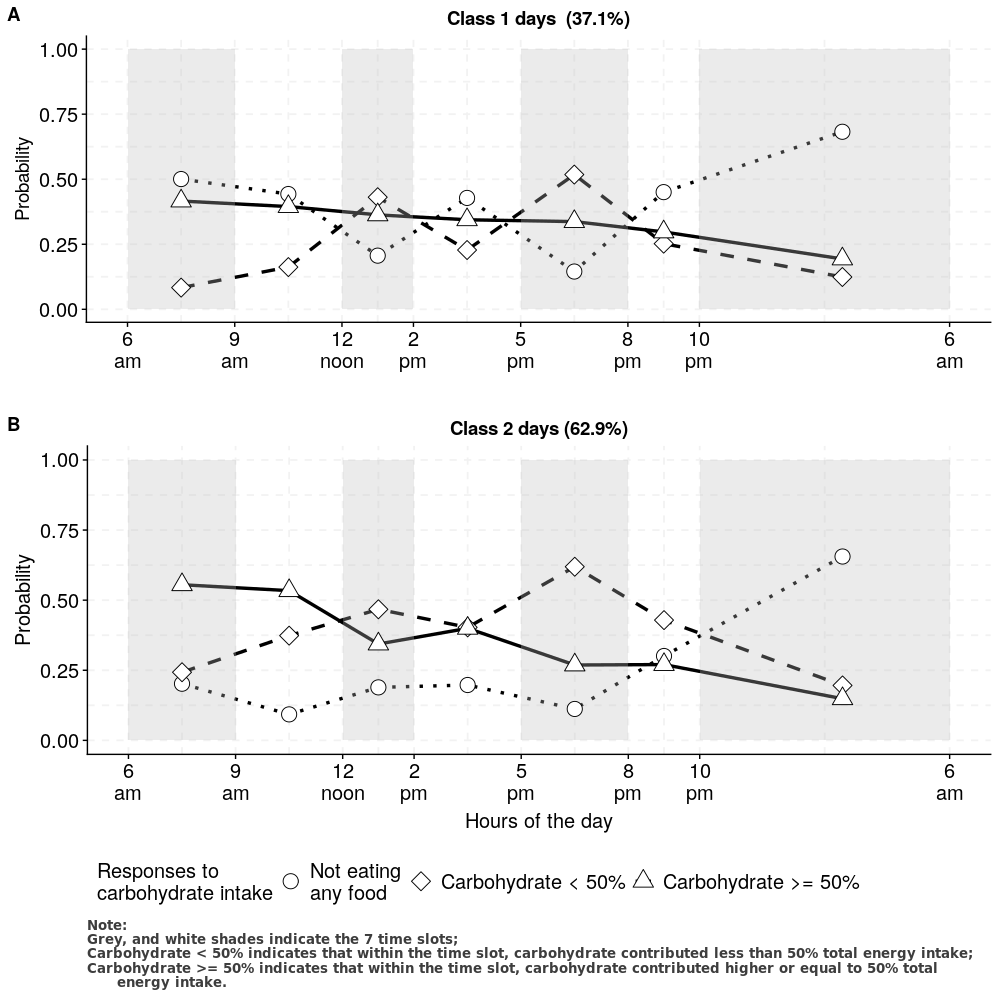
\includegraphics{Figures/CW2level1.png}
	\decoRule
	\caption[2 Classes solution in Day level]{2 Classes solution in Day level.}
	\label{fig:diary1}
\end{figure}



\begin{figure}[H]
	%\vspace*{13cm}
	\centering
	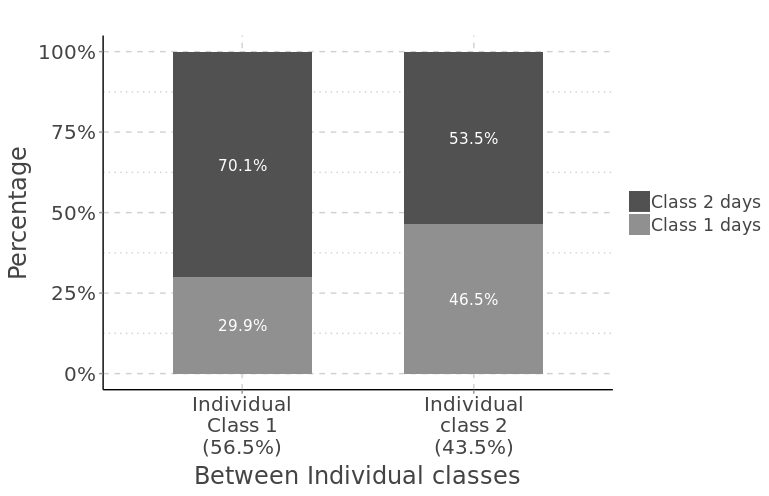
\includegraphics[width=13cm]{Figures/CW2CB2.png}
	\decoRule
	\caption[Multilevel Latent Class Solution (2 $\times$ 2).]{Multilevel Latent Class Solution, 2 classes in day level, 2 classes in individual level.}
	\label{fig:diary1}
\end{figure}




\begin{figure}[H]
	%\vspace*{13cm}
	\centering
	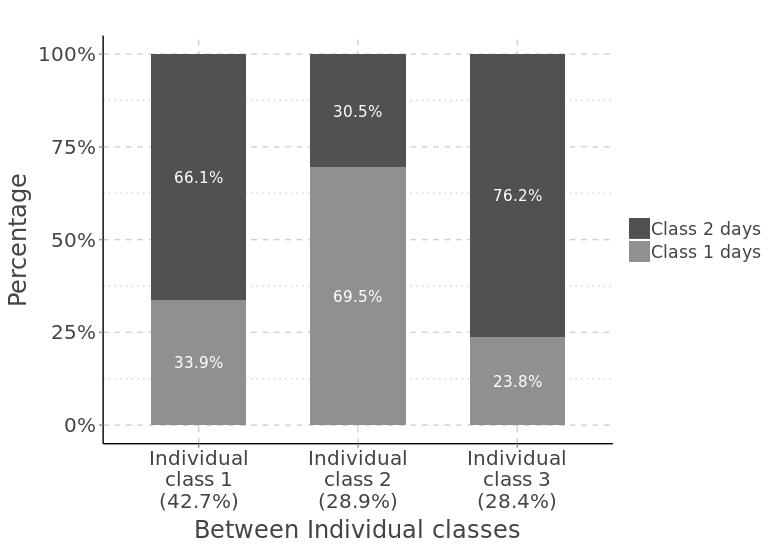
\includegraphics[width=13cm]{Figures/CW2CB3.png}
	\decoRule
	\caption[Multilevel Latent Class Solution (2 $\times$ 3).]{Multilevel Latent Class Solution, 2 classes in day level, 3 classes in individual level.}
	\label{fig:diary1}
\end{figure}


\begin{figure}[H]
	%\vspace*{13cm}
	\centering
	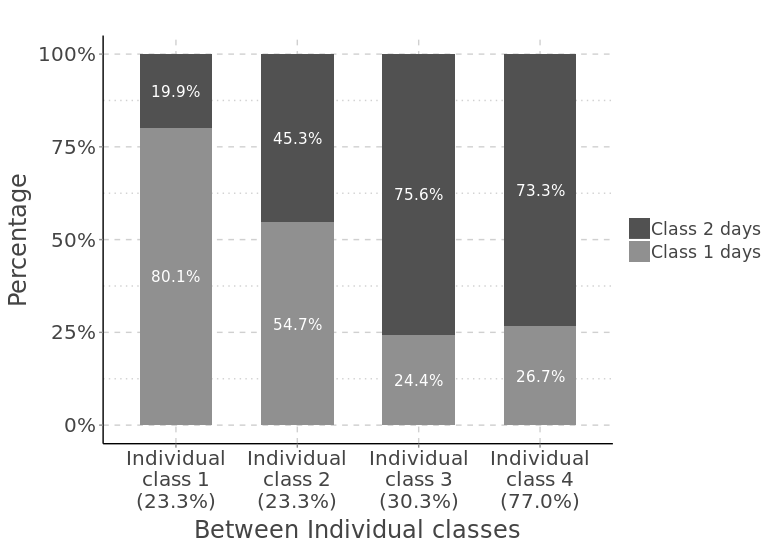
\includegraphics[width=13cm]{Figures/CW2CB4.png}
	\decoRule
	\caption[Multilevel Latent Class Solution (2 $\times$ 4).]{Multilevel Latent Class Solution, 2 classes in day level, 4 classes in individual level.}
	\label{fig:diary1}
\end{figure}

\section{3 classes in day level, 4 classes in individual level}\vspace{-0.3cm}

\begin{figure}[H]
	%\vspace*{13cm}
	\centering
	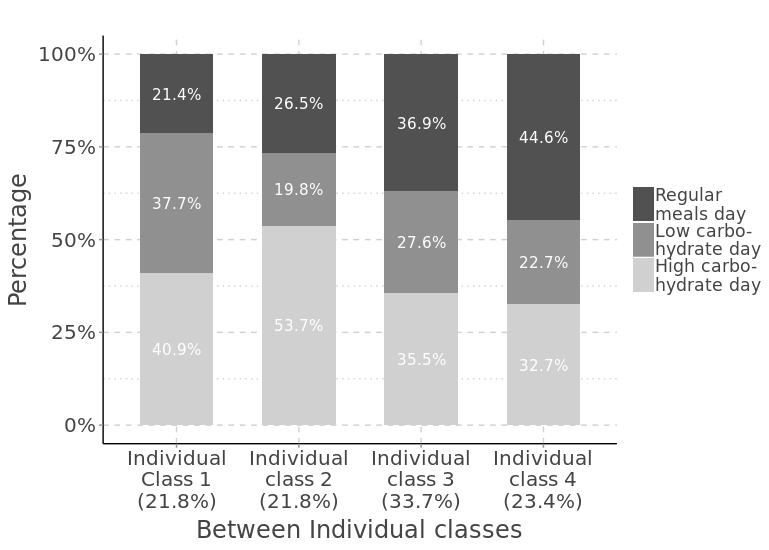
\includegraphics[width=13cm]{Figures/CW3CB4.png}
	\decoRule
	\caption[Multilevel Latent Class Solution (3 $\times$ 4).]{Multilevel Latent Class Solution, 3 classes in day level, 4 classes in individual level.}
	\label{fig:diary1}
\end{figure}


\section{4 classes in day level}

\begin{figure}[H]
	%\vspace*{13cm}
	\centering
	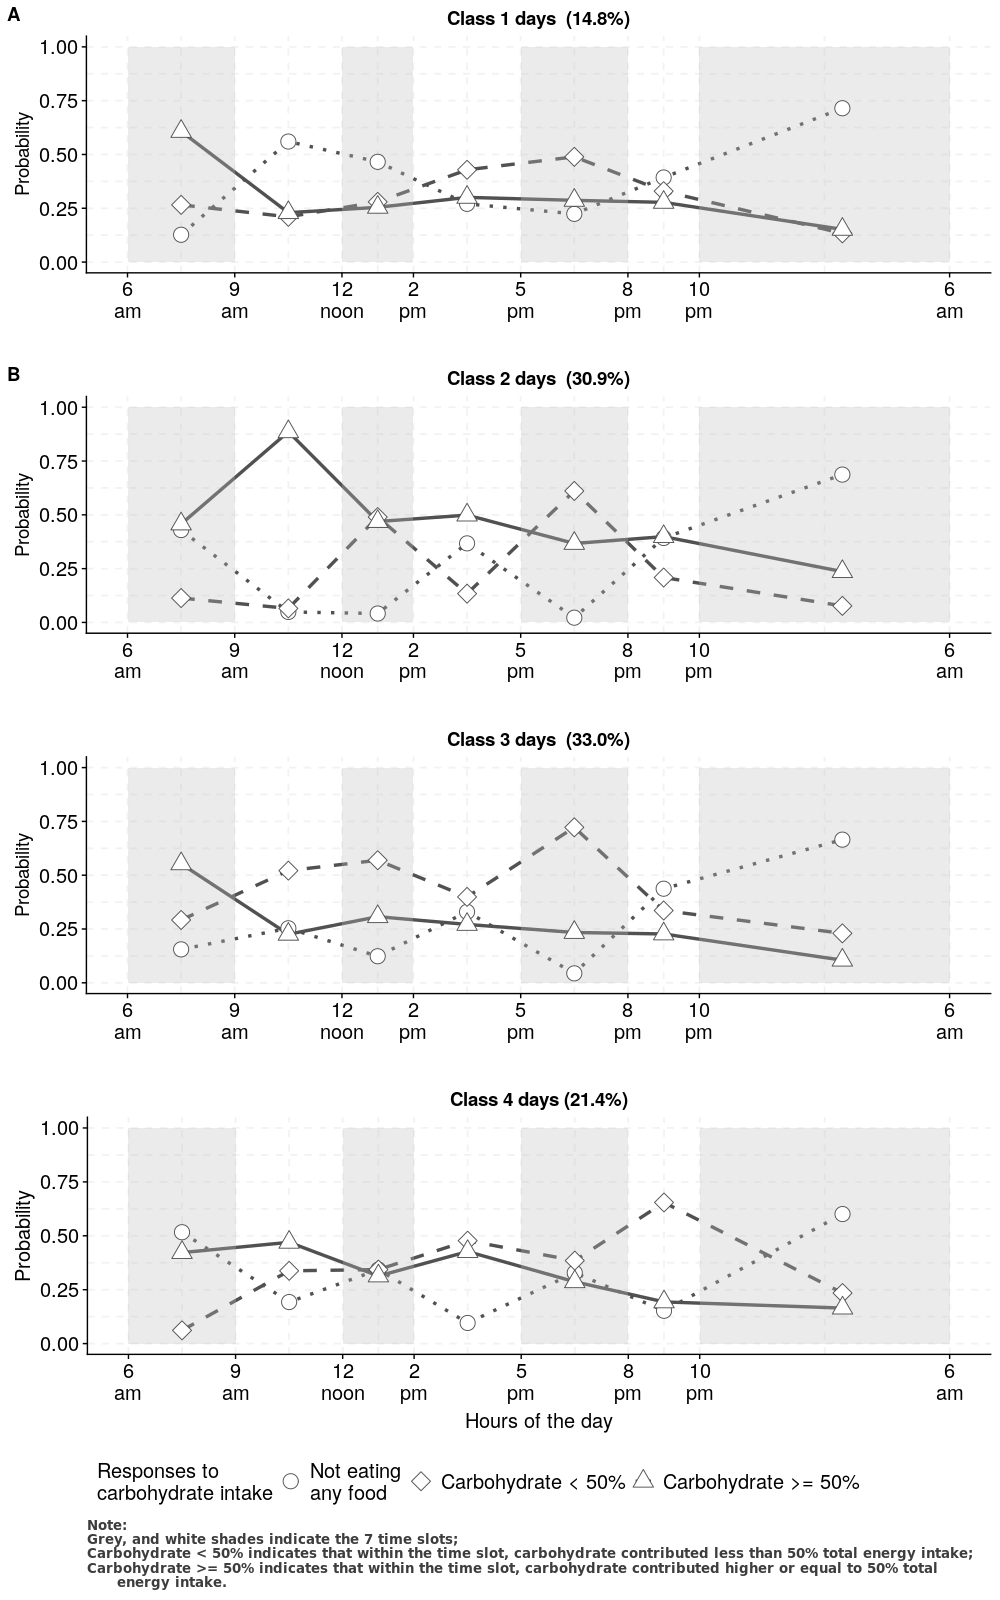
\includegraphics[width=15cm]{Figures/CW4level1.png}
	\decoRule
	\caption[2 Classes Solution in Day level]{4 Classes Solution in Day level.}
	\label{fig:diary1}
\end{figure}




%----------------------------------------------------------------------------------------

\end{document}
